\documentclass[a4paper,oneside,12pt]{book}

% ------------------------------------------------
% Codificación y lenguaje
% ------------------------------------------------
\usepackage[utf8]{inputenc}
\usepackage[T1]{fontenc}
\usepackage[spanish,es-lcroman,es-tabla]{babel}

% ------------------------------------------------
% Márgenes
% ------------------------------------------------
\usepackage[margin=1in]{geometry}

% ------------------------------------------------
% Matemáticas
% ------------------------------------------------
\usepackage{amsmath}
\usepackage{amssymb}
\usepackage{mathtools}

% ------------------------------------------------
% Figuras
% ------------------------------------------------
\usepackage{graphicx}
\graphicspath{{images/}{chapter_1/images_ch1/}}

\usepackage{float}
\usepackage{wrapfig}

% ------------------------------------------------
% Tablas
% ------------------------------------------------
\usepackage{booktabs}
\usepackage{tabularx}
\usepackage{longtable}

% ------------------------------------------------
% Colores
% ------------------------------------------------
\usepackage[table,xcdraw]{xcolor}

% ------------------------------------------------
% Subfiguras
% ------------------------------------------------
\usepackage{subcaption}

% ------------------------------------------------
% Espaciado
% ------------------------------------------------
\usepackage{setspace}

% ------------------------------------------------
% Encabezados
% ------------------------------------------------
\usepackage{fancyhdr}
\pagestyle{fancy}

\fancyhf{}
\fancyhead[L]{\leftmark}
\fancyhead[R]{\thepage}

\renewcommand{\headrulewidth}{0.4pt}
\setlength{\headheight}{15.13202pt}
\addtolength{\topmargin}{-3.13202pt}

% ------------------------------------------------
% Fuente (Times con soporte matemático completo; mathptmx reemplaza al
% paquete times antiguo y evita el error de fuente math al formatear URLs)
% ------------------------------------------------
\usepackage{mathptmx}

% ------------------------------------------------
% Párrafos
% ------------------------------------------------
\setlength{\parindent}{0pt}

% ------------------------------------------------
% BIBLIOGRAFÍA (Mendeley compatible)
% ------------------------------------------------
\usepackage[
backend=biber,
style=numeric,
sorting=none,
doi=true,
url=true,
isbn=false
]{biblatex}

% IMPORTANTE: Asegúrate de que el archivo que exportas de Mendeley se llame bibliografia.bib
\addbibresource{bibliografia.bib}

% --- SOLUCIÓN PARA GUIONES BAJOS DE MENDELEY ---
\DeclareSourcemap{
  \maps{
    \map{
      \step[fieldsource=doi, match=\regexp{\{\\\_\}|\{\_\}|\\\_}, replace=\regexp{\_}]
    }
    \map{
      \step[fieldsource=url, match=\regexp{\{\\\_\}|\{\_\}|\\\_}, replace=\regexp{\_}]
    }
  }
}
% --- FIN DE SOLUCIÓN MENDELEY ---

% ------------------------------------------------
% Hipervínculos (Debe cargarse al final de los paquetes)
% ------------------------------------------------
\usepackage{hyperref}


% =================================================
% DOCUMENTO
% =================================================

\begin{document}

% =================================================
% PORTADA 1 (Cubierta)
% =================================================

\begin{titlepage}

\begin{center}

% 1. Logo de la universidad (Encabezado visual)

\includegraphics[width=0.4\textwidth]{utp.jpg}

\vspace{1.5cm}

% 2. Título principal (Centro de atención)
{\LARGE \bfseries \linespread{1.3}\selectfont
Estudio de la Estabilidad de Métodos de Explicabilidad (XAI) en Graph Neural Networks para Detección de Lavado de Dinero bajo Desbalance Extremo de Datos\par}

\vspace{2.5cm}

% 3. Autores
{\Large
Alejandro Gómez Huertas \\[0.3cm]
Juan Diego Garzón Ovalle
}

\vfill

% 4. Información institucional (Bloque inferior sólido)
{\large
Universidad Tecnológica de Pereira \\
Facultad de Ingenierías \\
Maestría en Ingeniería en Sistemas y Computación \\
Pereira, Colombia \\
2026
}

\end{center}

\end{titlepage}

% =================================================
% PORTADA 2 (Portada Interna)
% =================================================

\begin{titlepage}

\begin{center}

\vspace*{1cm} % Margen superior para equilibrar la ausencia de logo

% 1. Título principal
{\LARGE \bfseries \linespread{1.3}\selectfont
Estudio de la Estabilidad de Métodos de Explicabilidad (XAI) en Graph Neural Networks para Detección de Lavado de Dinero bajo Desbalance Extremo de Datos\par}

\vspace{2cm}

% 2. Autores
{\Large
Alejandro Gómez Huertas \\[0.3cm]
Juan Diego Garzón Ovalle
}

\vspace{2.5cm}

% 3. Propósito académico (Redacción formal estándar)
{\large Tesis de grado presentada como requisito parcial para optar al título de:}\\[0.5cm]
{\Large \textbf{Magíster en Ingeniería en Sistemas y Computación}}

\vspace{2cm}

% 4. Director
{\large \textbf{Director} \\[0.2cm]
\Large Ph.D. Cristian Rosero Arias}

\vfill

% 5. Información institucional (Mismo bloque que la cubierta para consistencia)
{\large
Universidad Tecnológica de Pereira \\
Facultad de Ingenierías \\
Maestría en Ingeniería en Sistemas y Computación \\
Pereira, Colombia \\
2026
}

\end{center}

\end{titlepage}

% =================================================
% ÍNDICES
% =================================================

\pagenumbering{roman}

% =================================================
% RESUMEN / ABSTRACT
% =================================================

\chapter*{Resumen}
\addcontentsline{toc}{chapter}{Resumen}

La adopción de Graph Neural Networks (GNN) para la detección de lavado de dinero exige que sus predicciones sean explicables y que esas explicaciones resulten confiables en entornos regulados. Esta tesis estudia la estabilidad de tres métodos de explicabilidad post-hoc, GNNExplainer, PGExplainer y GNNShap, aplicados a cuatro arquitecturas, GCN, GraphSAGE, GAT y TAGCN, bajo niveles crecientes de desbalance de clases. Para superar la imposibilidad de medir la plausibilidad de las explicaciones sobre datos reales anonimizados, el trabajo adopta un diseño de dos ejes complementarios, el \textit{Elliptic Bitcoin Dataset}, que aporta validez externa, y un grafo sintético con \textit{ground-truth} por nodo y por arista, que aporta validez interna. Sobre una matriz factorial de sesenta configuraciones por eje, replicada con tres semillas de modelo y contrastada con pruebas no paramétricas e intervalos de confianza \textit{bootstrap}, se establecen tres resultados principales. Primero, la estabilidad, la plausibilidad y la fidelidad de las explicaciones son dimensiones empíricamente independientes, por lo que el mejor explicador depende del objetivo de la auditoría. Segundo, la estabilidad por arquitectura se organiza en dos grupos, uno alto formado por GAT y GCN y uno bajo por GraphSAGE y TAGCN, una partición que se reproduce de forma concordante en los dos regímenes de densidad. Tercero, el explicador más plausible no es el más fiel, una disociación que solo un régimen sintético controlado permite exhibir. El estudio corrige además dos artefactos de evaluación que invertían conclusiones sobre estabilidad, y condensa sus hallazgos en una matriz de recomendación según el objetivo operativo de la auditoría.

\vspace{0.4cm}
\noindent\textbf{Palabras clave:} redes neuronales de grafos, explicabilidad, estabilidad de las explicaciones, detección de lavado de dinero, desbalance de clases, \textit{Elliptic Bitcoin Dataset}, plausibilidad, fidelidad.

\chapter*{Abstract}
\addcontentsline{toc}{chapter}{Abstract}

The adoption of Graph Neural Networks (GNNs) for money laundering detection requires their predictions to be explainable and those explanations to be trustworthy in regulated settings. This thesis studies the stability of three post-hoc explainability methods, GNNExplainer, PGExplainer, and GNNShap, applied to four architectures, GCN, GraphSAGE, GAT, and TAGCN, under increasing levels of class imbalance. To overcome the impossibility of measuring explanation plausibility on anonymized real data, the work adopts a two-axis design, the \textit{Elliptic Bitcoin Dataset}, which provides external validity, and a synthetic graph with per-node and per-edge \textit{ground-truth}, which provides internal validity. Over a factorial matrix of sixty configurations per axis, replicated with three model seeds and assessed with nonparametric tests and \textit{bootstrap} confidence intervals, three main results are established. First, the stability, plausibility, and fidelity of explanations are empirically independent dimensions, so the best explainer depends on the auditing goal. Second, architecture stability organizes into two groups, a high group formed by GAT and GCN and a low group by GraphSAGE and TAGCN, a partition that reproduces concordantly across both density regimes. Third, the most plausible explainer is not the most faithful, a dissociation that only a controlled synthetic regime can exhibit. The study further corrects two evaluation artifacts that had inverted stability conclusions, and condenses its findings into a recommendation matrix by operational auditing objective.

\vspace{0.4cm}
\noindent\textbf{Keywords:} graph neural networks, explainability, explanation stability, money laundering detection, class imbalance, \textit{Elliptic Bitcoin Dataset}, plausibility, fidelity.

\clearpage

\tableofcontents

\newpage
\listoffigures
\addcontentsline{toc}{chapter}{Índice de figuras}

\newpage
\listoftables
\addcontentsline{toc}{chapter}{Índice de tablas}

% =================================================
% LISTA DE ACRONIMOS
% =================================================

\newpage
\chapter*{Lista de Acrónimos}
\addcontentsline{toc}{chapter}{Lista de Acrónimos}

\begin{longtable}{p{0.16\textwidth}p{0.78\textwidth}}
\textbf{AML} & \textit{Anti-Money Laundering}, prevención del lavado de activos \\[2pt]
\textbf{AUC-PR} & Área bajo la curva de precisión y exhaustividad (\textit{Precision-Recall Area Under the Curve}) \\[2pt]
\textbf{FATF} & \textit{Financial Action Task Force} (Grupo de Acción Financiera Internacional) \\[2pt]
\textbf{GAFI} & Grupo de Acción Financiera Internacional \\[2pt]
\textbf{GAT} & \textit{Graph Attention Network}, red de grafos con atención \\[2pt]
\textbf{GCN} & \textit{Graph Convolutional Network}, red convolucional de grafos \\[2pt]
\textbf{GNN} & \textit{Graph Neural Network}, red neuronal de grafos \\[2pt]
\textbf{GraphSAGE} & \textit{Graph Sample and Aggregate} \\[2pt]
\textbf{GraphSMOTE} & \textit{Graph Synthetic Minority Over-sampling Technique} \\[2pt]
\textbf{KYC} & \textit{Know Your Customer}, conocimiento del cliente \\[2pt]
\textbf{LSTM} & \textit{Long Short-Term Memory}, memoria larga a corto plazo \\[2pt]
\textbf{MCC} & Coeficiente de correlación de Matthews (\textit{Matthews Correlation Coefficient}) \\[2pt]
\textbf{PCA} & Análisis de componentes principales (\textit{Principal Component Analysis}) \\[2pt]
\textbf{PR-AUC} & Área bajo la curva de precisión y exhaustividad (\textit{Precision-Recall Area Under the Curve}) \\[2pt]
\textbf{ReLU} & \textit{Rectified Linear Unit}, unidad lineal rectificada \\[2pt]
\textbf{ROC-AUC} & Área bajo la curva característica operativa del receptor (\textit{Receiver Operating Characteristic Area Under the Curve}) \\[2pt]
\textbf{SHAP} & \textit{SHapley Additive exPlanations} \\[2pt]
\textbf{SMOTE} & \textit{Synthetic Minority Over-sampling Technique} \\[2pt]
\textbf{TAGCN} & \textit{Topology Adaptive Graph Convolutional Network} \\[2pt]
\textbf{t-SNE} & \textit{t-distributed Stochastic Neighbor Embedding} \\[2pt]
\textbf{VASP} & \textit{Virtual Asset Service Provider}, proveedor de servicios de activos virtuales \\[2pt]
\textbf{XAI} & Inteligencia artificial explicable (\textit{Explainable Artificial Intelligence}) \\[2pt]
\end{longtable}

% =================================================
% CONTENIDO
% =================================================

\newpage
\pagenumbering{arabic}

\chapter{INTRODUCCIÓN}

\section{Planteamiento y Contexto del Problema}

El lavado de dinero, designado en la literatura internacional como \textit{Anti-Money Laundering} (AML), constituye uno de los mecanismos centrales mediante los cuales las economías criminales logran insertar recursos ilícitos dentro de los circuitos financieros formales. Este fenómeno facilita la circulación de capitales provenientes del narcotráfico, la trata de personas, el tráfico de armas, la corrupción o el financiamiento del terrorismo, y al mismo tiempo erosiona la estabilidad institucional, distorsiona los mercados y debilita la confianza en los sistemas de supervisión financiera. Su magnitud ha dejado de ser un asunto exclusivamente policial para convertirse en un problema económico y regulatorio de escala global. En este sentido, se ha estimado que los flujos financieros ilícitos representan entre el 2\% y el 5\% del Producto Interno Bruto mundial, lo cual equivale a montos cercanos a los 2 billones de dólares anuales \cite{UNODC2024EstimatingCrimes}.

\bigskip

En el caso particular de las criptomonedas, el problema adquiere una complejidad adicional. La arquitectura descentralizada de los sistemas \textit{blockchain}, la facilidad para transferir valor de forma transfronteriza, el seudonimato de las direcciones y la ausencia de intermediarios tradicionales han creado un entorno atractivo para la circulación, fragmentación y ocultamiento de fondos ilícitos \cite{Spotlight2021Cryptocurrencies:Finances, Subashi2024CryptocurrenciesLaundering}. A esto se suma la sofisticación creciente de las técnicas de lavado basadas en criptoactivos, las cuales ya no se limitan a transferencias simples, sino que incluyen estrategias de dispersión, mezcla, integración y transacciones encadenadas que aprovechan la estructura de red de los ecosistemas digitales \cite{Almeida2025FromTechniques}. Como resultado, la detección de operaciones sospechosas en este contexto exige modelos capaces de comprender relaciones dinámicas y patrones estructurales más allá del análisis aislado de transacciones individuales.

\bigskip

Las instituciones financieras y los \textit{exchanges} de criptomonedas continúan dependiendo, en gran medida, de Sistemas de Monitoreo de Transacciones (TMS) convencionales, sustentados en reglas deterministas, listas de vigilancia y umbrales estáticos. Aunque estas herramientas han sido la base del cumplimiento normativo durante décadas, su capacidad para responder a tipologías modernas de lavado es limitada. El principal problema radica en que tratan las transacciones como eventos independientes, ignorando la topología relacional entre cuentas, billeteras y flujos monetarios. Esto produce un ruido operativo masivo: diversos estudios reportan que entre el 95\% y el 98\% de las alertas generadas por estos sistemas corresponden a falsos positivos \cite{Unagar2025SurveyXAI}. En consecuencia, los equipos de cumplimiento deben invertir enormes cantidades de tiempo y recursos en la revisión manual de alertas irrelevantes, mientras que los patrones verdaderamente sofisticados logran mimetizarse dentro del volumen general de actividad financiera.

\bigskip

Este problema de ineficiencia no es únicamente técnico, sino también económico y estratégico. Los falsos positivos elevan de manera desproporcionada los costos de operación, reducen la capacidad de respuesta analítica de las instituciones y generan fatiga organizacional en los procesos de monitoreo. Más grave aún, desplazan la atención desde los casos realmente relevantes hacia señales espurias que no representan riesgo material. En otras palabras, un sistema que produce demasiadas alertas incorrectas falla en dos direcciones a la vez, por exceso y por omisión: al saturar la capacidad investigativa, incrementa la probabilidad de que operaciones ilícitas genuinas pasen desapercibidas \cite{Subashi2024CryptocurrenciesLaundering, Unagar2025SurveyXAI}. Esta realidad ha impulsado la búsqueda de modelos más robustos que puedan capturar estructuras complejas de interacción financiera sin depender exclusivamente de reglas manuales.

\bigskip

En este escenario, las \textit{Graph Neural Networks} (GNNs) han emergido como un paradigma prometedor para el dominio AML. A diferencia de los modelos tabulares tradicionales, las GNNs explotan explícitamente la naturaleza relacional de los datos financieros, representando las transacciones y entidades como nodos, y sus vínculos como aristas dentro de un grafo. Esta formulación permite aprender patrones topológicos que serían invisibles para modelos clásicos, tales como vecindarios sospechosos, cadenas de dispersión, ciclos transaccionales o estructuras de intermediación artificial \cite{Weber2019Anti-MoneyForensics, Lawal2025AnDataset}. Los trabajos pioneros sobre el \textit{Elliptic Dataset} mostraron que el modelado basado en grafos supera a varios enfoques convencionales en la detección de transacciones ilícitas sobre redes de Bitcoin, precisamente porque integra información estructural y contextual en el proceso de clasificación \cite{Weber2019Anti-MoneyForensics}.

\bigskip

La evolución reciente de este campo ha dado lugar a arquitecturas aún más especializadas. Por ejemplo, modelos híbridos que integran dinámicas temporales y convoluciones sobre grafos han mostrado que la detección AML mejora cuando se considera simultáneamente la dependencia estructural y la evolución secuencial de las transacciones \cite{Alarab2023Graph-basedData, Wan2024AMemory}. Asimismo, arquitecturas con mecanismos de atención y variantes de grafos evolutivos han ampliado la capacidad de capturar dependencias de largo alcance y cambios temporales en comportamientos ilícitos \cite{Cui2024EG-SAN:Cryptocurrency, Lin2026DetectingLaundering}. Dentro de este ecosistema, TAGCN (\textit{Topology Adaptive Graph Convolutional Network}) resulta particularmente interesante, ya que incorpora filtros polinomiales adaptativos capaces de agregar información desde múltiples saltos topológicos, permitiendo modelar dependencias más complejas que las capturadas por esquemas puramente locales \cite{Du2017TopologyNetworks, He2026AnDetection}.

\bigskip

Sin embargo, el uso de GNNs en contextos regulados introduce una tensión crítica entre desempeño predictivo y auditabilidad. A pesar de su potencia analítica, estas arquitecturas funcionan como modelos altamente opacos, lo que dificulta comprender qué patrones concretos justifican una predicción de riesgo. En dominios como AML, esta opacidad es especialmente problemática, ya que las decisiones automatizadas pueden derivar en bloqueos de cuentas, reportes de operaciones sospechosas o investigaciones con implicaciones jurídicas y reputacionales significativas \cite{FATF2012InternationalRecommendations, Spotlight2021Cryptocurrencies:Finances}. Por ello, la exigencia contemporánea ya no es únicamente construir sistemas más precisos, sino desarrollar sistemas que además sean interpretables, auditables y defendibles frente a reguladores y equipos de cumplimiento.

\bigskip

En respuesta a esta necesidad, la Inteligencia Artificial Explicable (\textit{Explainable AI}, XAI) se ha consolidado como una línea de investigación central para reducir la opacidad de los modelos complejos. En el caso de las GNNs, los métodos XAI buscan identificar qué nodos, aristas, atributos o subgrafos influyen de forma decisiva en una predicción concreta \cite{Adadi2018PeekingXAI, Ying2019Gnnexplainer:Networks, Luo2020ParameterizedNetwork, Akkas2024Gnnshap:Values}. No obstante, la literatura reciente ha mostrado que la generación de explicaciones para modelos de grafos enfrenta limitaciones profundas asociadas con su fidelidad, robustez e inestabilidad. En particular, explicaciones obtenidas sobre una misma instancia pueden variar considerablemente entre ejecuciones o bajo pequeñas perturbaciones, lo que cuestiona su confiabilidad como soporte analítico o forense \cite{Gawantka2024AExplanations, Agarwal2022ProbingMethods,Kosan2023GNNX-BENCH:Benchmarking}. Esta problemática constituye el núcleo conceptual de la presente investigación.

\bigskip

\section{Revisión de Literatura y Estado del Arte}

La literatura reciente sobre detección de lavado de dinero en criptomonedas muestra una evolución progresiva desde enfoques transaccionales convencionales hacia modelos estructurales basados en grafos. En una primera etapa, los trabajos se concentraron en adaptar algoritmos clásicos de clasificación al problema AML, utilizando atributos tabulares extraídos de cada transacción, como montos, frecuencia, temporalidad y estadísticas agregadas. Aunque estos métodos ofrecieron una base importante para automatizar el análisis de riesgo, su principal limitación fue la incapacidad de capturar la dependencia relacional entre transacciones y entidades, una dimensión central en las tipologías de lavado \cite{Weber2019Anti-MoneyForensics, Unagar2025SurveyXAI}.

\bigskip

El trabajo de Weber et al. constituye un punto de inflexión en esta línea, pues introdujo el uso del \textit{Elliptic Dataset} como entorno de experimentación para modelos basados en grafos sobre transacciones Bitcoin. Su estudio mostró que representar la red de transacciones como un grafo permite capturar patrones estructurales que los modelos tabulares pierden, logrando mejoras consistentes en la clasificación de actividad ilícita \cite{Weber2019Anti-MoneyForensics}. Este aporte fue determinante porque transformó el problema AML desde una perspectiva centrada en instancias individuales hacia una perspectiva relacional, donde la posición de una transacción dentro de la red es tan importante como sus atributos intrínsecos.

\bigskip

A partir de este cambio de paradigma, surgieron múltiples variantes de GNNs aplicadas al dominio financiero. Lawal et al. propusieron un marco explicable para detección AML en criptomonedas utilizando el \textit{Elliptic Dataset}, demostrando que los modelos de grafos mejoran el rendimiento predictivo y admiten su combinación con mecanismos de explicabilidad post-hoc \cite{Lawal2025AnDataset}. Por su parte, He et al. desarrollaron un marco explicable para la detección de transacciones financieras ilícitas, reforzando la idea de que el futuro de estos sistemas no pasa únicamente por maximizar métricas predictivas, sino por integrar interpretabilidad como componente esencial del diseño \cite{He2026AnDetection}.

\bigskip

La investigación también ha explorado arquitecturas dinámicas e híbridas. Alarab y Prakoonwit estudiaron un modelo \textit{graph-based LSTM} que combina componentes temporales con procesamiento estructural de grafos, mostrando que la dimensión temporal puede aportar valor cuando las actividades ilícitas se distribuyen a lo largo de secuencias transaccionales \cite{Alarab2023Graph-basedData}. De manera similar, Wan y Li propusieron un modelo de predicción de lavado basado en una red convolucional dinámica sobre grafos y una arquitectura LSTM, reforzando la hipótesis de que el comportamiento ilícito no es estático, sino evolutivo \cite{Wan2024AMemory}. Estos trabajos abren la puerta a sistemas más realistas para entornos donde las redes transaccionales cambian continuamente en el tiempo.

\bigskip

En paralelo, otros autores han investigado mecanismos de atención y aprendizaje estructural avanzado. Cui y Zhang presentaron EG-SAN, un modelo de autoatención sobre grafos evolutivos para detectar actividades ilícitas en criptomonedas, destacando el valor de ponderar selectivamente la relevancia de diferentes conexiones dentro de la red \cite{Cui2024EG-SAN:Cryptocurrency}. Xu et al. también exploraron redes de autoatención para AML, enfatizando la capacidad de estas arquitecturas para identificar patrones de dependencia más refinados que los capturados por esquemas de agregación uniformes \cite{Lin2026DetectingLaundering}. De forma complementaria, Lo et al. propusieron \textit{Inspection-L}, un enfoque auto-supervisado para aprender representaciones de nodos aplicadas a la detección de lavado de dinero, lo cual evidencia que la literatura también avanza hacia estrategias menos dependientes de grandes cantidades de etiquetas balanceadas \cite{Lo2023Inspection-L:Bitcoin}.

\bigskip

No obstante, la evolución de las arquitecturas predictivas no ha sido acompañada de una evolución igualmente sólida en los mecanismos de validación explicativa. Los métodos XAI para GNNs han crecido rápidamente en número y diversidad, pero aún presentan desafíos importantes. GNNExplainer, propuesto por Ying et al., se consolidó como uno de los primeros métodos capaces de identificar subgrafos y atributos relevantes para justificar una predicción de GNN \cite{Ying2019Gnnexplainer:Networks}. Posteriormente, PGExplainer introdujo un enfoque parametrizado que aprende un generador de explicaciones, mejorando escalabilidad y generalización frente a enfoques puramente locales \cite{Luo2020ParameterizedNetwork}. Más recientemente, GNNShap adaptó la lógica de los valores de Shapley al contexto de grafos, buscando explicaciones más consistentes y teóricamente fundamentadas \cite{Akkas2024Gnnshap:Values}.

\bigskip

A pesar de estos avances, la literatura coincide en que explicar GNNs sigue siendo un problema abierto. Distintos marcos sistemáticos para evaluar métodos de explicabilidad en redes de grafos han mostrado que muchas explicaciones consideradas plausibles no necesariamente son fieles ni robustas \cite{Armgaan2025GnnXemplar:Interpretability}. En una línea similar, Agarwal et al. realizaron un análisis riguroso de los métodos explicadores para GNNs y evidenciaron limitaciones tanto teóricas como prácticas en su capacidad para reflejar con precisión el razonamiento interno del modelo \cite{Agarwal2022ProbingMethods}. Kosan et al., mediante GNNX-BENCH, reforzaron esta crítica al demostrar que el desempeño de los explicadores depende fuertemente del criterio de evaluación utilizado, y que muchos resultados reportados en la literatura son sensibles al protocolo experimental \cite{Kosan2023GNNX-BENCH:Benchmarking}.

\bigskip

En el dominio AML, esta limitación es todavía más delicada. No basta con que un explicador produzca un subgrafo visualmente coherente; es necesario que la explicación sea estable, reproducible y suficientemente fiel como para respaldar decisiones en escenarios regulados. Gawantka et al. propusieron una métrica específica para evaluar la estabilidad de las explicaciones XAI, subrayando que este criterio ha sido históricamente subestimado en la literatura \cite{Gawantka2024AExplanations}. A su vez, Rai et al. mostraron que el desbalance de clases puede deteriorar significativamente el comportamiento de las técnicas XAI, incluso cuando el modelo mantiene un desempeño predictivo aceptable \cite{Rai2025EvaluatingData}. Fujiwara profundizó en esta relación al estudiar cómo técnicas de remuestreo y destilación del conocimiento pueden mejorar simultáneamente el rendimiento predictivo y la estabilidad explicativa en escenarios desbalanceados \cite{Fujiwara2024KnowledgeStability}.

\bigskip

En consecuencia, el estado del arte revela una convergencia clara: el problema AML en criptomonedas requiere modelos estructurales capaces de captar relaciones complejas, pero también exige mecanismos de explicabilidad cuya calidad no se mida únicamente por intuición visual o plausibilidad superficial. La combinación entre GNNs, XAI y desbalance extremo sigue siendo una zona insuficientemente explorada, especialmente cuando el criterio central de evaluación no es solo la exactitud de la clasificación, sino la estabilidad y auditabilidad de la explicación obtenida \cite{Unagar2025SurveyXAI, Gawantka2024AExplanations, Rai2025EvaluatingData}.

\bigskip

\begin{table}[h!]
\centering
\begin{tabular}{|p{3.2cm}|p{3.7cm}|p{4.2cm}|p{4.2cm}|}
\hline
\textbf{Trabajo} & \textbf{Enfoque principal} & \textbf{Aporte} & \textbf{Limitación relevante} \\
\hline
Weber et al. \cite{Weber2019Anti-MoneyForensics} & GCN sobre Bitcoin & Introduce el modelado relacional con Elliptic Dataset & Limitada atención a explicabilidad \\
\hline
Lawal et al. \cite{Lawal2025AnDataset} & GNN explicable para AML & Integra predicción y explicación en cripto AML & No profundiza en estabilidad bajo desbalance extremo \\
\hline
He et al. \cite{He2026AnDetection} & Framework explicable para transacciones ilícitas & Refuerza la necesidad de interpretabilidad en finanzas & Requiere validación exhaustiva de robustez explicativa \\
\hline
Wan y Li \cite{Wan2024AMemory} & GCN dinámica + LSTM & Modela dependencias estructurales y temporales & Mayor complejidad experimental \\
\hline
Cui y Zhang \cite{Cui2024EG-SAN:Cryptocurrency} & Autoatención en grafos evolutivos & Mejora detección en grafos dinámicos & Explicabilidad no es el foco central \\
\hline
Gawantka et al. \cite{Gawantka2024AExplanations} & Métrica de estabilidad XAI & Formaliza la evaluación de estabilidad explicativa & No se centra específicamente en AML \\
\hline
Rai et al. \cite{Rai2025EvaluatingData} & XAI bajo desbalance & Evidencia impacto del desbalance sobre explicaciones & Estudio en otro dominio, no sobre grafos AML \\
\hline
Fujiwara \cite{Fujiwara2024KnowledgeStability} & Remuestreo y estabilidad explicativa & Relaciona balanceo con estabilidad XAI & No aborda GNNs financieras de forma directa \\
\hline
\end{tabular}
\caption{Síntesis del estado del arte en detección AML basada en grafos y explicabilidad}
\end{table}

\section{La Arista de Investigación}

A pesar del avance significativo en la detección de lavado de dinero con modelos basados en grafos, la literatura actual exhibe una desconexión evidente entre tres dimensiones que deberían estudiarse de manera integrada: el desbalance extremo de clases, la calidad de las explicaciones XAI y la robustez estructural de las arquitecturas GNN. Esta desconexión constituye la brecha central que motiva la presente investigación. Si bien existen trabajos que mejoran el rendimiento predictivo, trabajos que desarrollan explicadores para GNNs y trabajos que analizan estabilidad explicativa en otros dominios, todavía no existe una evaluación sistemática de cómo estas tres dimensiones interactúan en un entorno AML realista.

\bigskip

En primer lugar, el desbalance extremo de datos sigue siendo tratado de forma insuficiente. En los escenarios reales de monitoreo financiero, la clase ilícita representa una fracción minúscula del total de transacciones, pudiendo llegar a razones cercanas a 1:1000 o incluso más severas dependiendo del contexto operacional \cite{Rai2025EvaluatingData, Unagar2025SurveyXAI}. Sin embargo, una parte importante de la literatura experimental evalúa modelos en condiciones relativamente benignas, con particiones de datos que no reflejan la escasez real de eventos ilícitos. Esta simplificación puede inflar artificialmente el rendimiento del clasificador y ocultar el deterioro que ocurre cuando el sistema debe operar en ambientes altamente desbalanceados. Técnicas como GraphSMOTE han sido propuestas para clasificación desbalanceada en grafos, pero su efecto sobre la explicación generada por el modelo sigue siendo una cuestión abierta \cite{Zhao2021Graphsmote:Networks}.

\bigskip

En segundo lugar, la literatura no ha resuelto satisfactoriamente el problema de la fidelidad y la estabilidad explicativa. La mayoría de los trabajos en XAI para grafos se ha enfocado en producir explicaciones plausibles o visualmente intuitivas, pero no necesariamente en demostrar que estas explicaciones son consistentes entre ejecuciones, robustas frente a perturbaciones o verdaderamente representativas del mecanismo de decisión interno del modelo \cite{Agarwal2022ProbingMethods, Armgaan2025GnnXemplar:Interpretability, Kosan2023GNNX-BENCH:Benchmarking}. En contextos como AML, esta omisión es particularmente crítica, ya que una explicación inestable carece de valor operativo y jurídico. Una entidad financiera no puede sustentar una alerta de alto impacto en un subgrafo explicativo que cambia de forma sustancial cada vez que el explicador se ejecuta sobre la misma transacción.

\bigskip

En tercer lugar, la relación entre estrategias de mitigación del desbalance y calidad explicativa permanece subexplorada. Rai et al. y Fujiwara mostraron que el desbalance afecta tanto al clasificador como a la consistencia de las explicaciones, y que ciertas técnicas de remuestreo pueden modificar esta relación \cite{Rai2025EvaluatingData, Fujiwara2024KnowledgeStability}. Sin embargo, estos hallazgos no se han extendido de forma rigurosa al dominio AML basado en grafos, donde la inserción de nodos sintéticos, el ajuste de pesos o el uso de funciones de pérdida especializadas podrían alterar la topología original y, con ello, introducir sesgos o artefactos en las explicaciones. En otras palabras, aún no está claro si balancear los datos mejora la comprensión del fenómeno ilícito o si, por el contrario, fabrica una representación más conveniente para el clasificador pero menos fiel al comportamiento real de la red financiera.

\bigskip

También existe una brecha comparativa entre arquitecturas. La literatura ha mostrado resultados prometedores con GCN, GraphSAGE, GAT, TAGCN, modelos temporales y modelos de atención, pero no ha establecido con claridad cuál de estas arquitecturas ofrece mejores garantías de interpretabilidad estable bajo condiciones severas de desbalance \cite{Weber2019Anti-MoneyForensics, Lin2026DetectingLaundering, Cui2024EG-SAN:Cryptocurrency, Du2017TopologyNetworks, He2026AnDetection}. El problema no consiste únicamente en identificar qué arquitectura clasifica mejor, sino en determinar cuál produce explicaciones más consistentes, robustas y utilizables en contextos regulatorios. Este es un vacío importante, porque una arquitectura con un desempeño predictivo ligeramente superior podría ser menos deseable si sus explicaciones son erráticas o frágiles.

\bigskip

En síntesis, la literatura no ha respondido de manera integral a la siguiente cuestión: ¿cómo se comportan los métodos XAI aplicados a distintas arquitecturas GNN para detección AML cuando el sistema enfrenta niveles extremos de desbalance, y qué combinación de arquitectura, explicador y estrategia de balanceo ofrece el mejor compromiso entre rendimiento predictivo y estabilidad explicativa? Esta ausencia de evidencia comparativa y metodológicamente rigurosa constituye la brecha específica que esta tesis busca cerrar.

\bigskip

\section{Formulación del Problema}

A partir del contexto presentado y de la revisión del estado del arte, se identifica un vacío de investigación en la evaluación rigurosa de la estabilidad de los métodos de explicabilidad aplicados a modelos GNN en escenarios AML caracterizados por desbalance extremo de datos. Este vacío no es menor: compromete la posibilidad de trasladar los avances en detección basada en grafos hacia entornos donde la auditabilidad, la reproducibilidad y la trazabilidad de la decisión son condiciones indispensables.

\bigskip

El problema no se reduce a mejorar métricas de clasificación. De hecho, una parte relevante de la literatura reciente ya ha mostrado que es posible obtener mejoras sustanciales en tareas de detección AML mediante arquitecturas de grafos, mecanismos de atención o modelos híbridos \cite{Lawal2025AnDataset, Wan2024AMemory, Lin2026DetectingLaundering}. Sin embargo, cuando se introduce la dimensión explicativa, emergen limitaciones todavía no resueltas: las explicaciones pueden ser inestables, sensibles al ruido topológico, dependientes del método explicador e incluso afectadas por las estrategias utilizadas para compensar el desbalance de clases \cite{Gawantka2024AExplanations, Rai2025EvaluatingData, Fujiwara2024KnowledgeStability}. En consecuencia, el problema científico de esta tesis se sitúa en la intersección entre clasificación, interpretabilidad y robustez. Para abordarlo, la investigación articula dos ejes complementarios, el primero sobre el \textit{Elliptic Dataset} de transacciones reales de Bitcoin y el segundo sobre un grafo sintético con \textit{ground-truth} de tipología que hace medible la plausibilidad de las explicaciones, y sostiene sus conclusiones mediante un análisis estadístico basado en réplicas por semilla, intervalos de confianza y pruebas no paramétricas.

\bigskip

\textbf{Problema Principal:}\\
¿Cómo evaluar y cuantificar la degradación de la estabilidad de los métodos de explicabilidad (XAI) en arquitecturas de \textit{Graph Neural Networks} (GNNs) aplicadas a la detección de lavado de dinero en transacciones de Bitcoin sobre el \textit{Elliptic Dataset}, bajo condiciones severas de desbalance de datos, y qué estrategias de balanceo y selección de modelos logran maximizar la estabilidad explicativa sin sacrificar el rendimiento predictivo?

\bigskip

\textbf{Problemas Específicos:}
\begin{itemize}
    \item ¿Cómo se cuantifica de forma verificable la degradación en la estabilidad de las explicaciones estructurales generadas por métodos XAI de diferente naturaleza, como GNNExplainer, PGExplainer y GNNShap, a medida que la razón de desbalance de clases se hace más extrema \cite{Ying2019Gnnexplainer:Networks, Luo2020ParameterizedNetwork, Akkas2024Gnnshap:Values}?
    \item ¿De qué manera las diferencias estructurales y mecanismos de agregación intrínsecos de diversas arquitecturas GNN, tales como GCN, GraphSAGE, GAT y TAGCN, condicionan la robustez de las explicaciones resultantes frente al ruido topológico presente en un grafo financiero \cite{Du2017TopologyNetworks, He2026AnDetection}?
    \item ¿Cuál es el impacto colateral de implementar técnicas de sobremuestreo topológico o ajuste de pesos, como GraphSMOTE o funciones de pérdida orientadas al desbalance, sobre la interpretabilidad del modelo \cite{Zhao2021Graphsmote:Networks}?
    \item ¿Es posible identificar una combinación sinérgica entre arquitectura de red, algoritmo explicador y estrategia de mitigación del desbalance que maximice simultáneamente la fidelidad predictiva y la estabilidad explicativa, sirviendo como referencia para sistemas AML auditables?
\end{itemize}

\bigskip

\section{Objetivos}

La presente investigación establece un marco de objetivos orientado a estudiar de manera sistemática la estabilidad de las explicaciones generadas por modelos GNN en escenarios AML con desbalance extremo. Más que proponer una mejora incremental en precisión, se busca construir evidencia robusta y verificable que permita entender el comportamiento explicativo de estas arquitecturas en condiciones cercanas a las del dominio real.

\subsection{Objetivo General}

Evaluar exhaustivamente la estabilidad de los métodos de explicabilidad en Redes Neuronales de Grafos bajo condiciones extremas de desbalance de datos en la detección de lavado de dinero sobre el \textit{Elliptic Dataset}, con el fin de proporcionar evidencia rigurosa y recomendaciones técnicas sobre las combinaciones óptimas de arquitectura, explicador y técnica de balanceo que garanticen explicaciones robustas, consistentes y auditables en entornos regulados.

\bigskip

\subsection{Objetivos Específicos}

\begin{itemize}
    \item Evaluar el impacto directo del desequilibrio de clases en la robustez de las explicaciones estructurales, ejecutando un análisis comparativo y cuantitativo de métodos representativos como GNNExplainer, PGExplainer y GNNShap a través de escenarios incrementales de submuestreo y desbalance en el \textit{Elliptic Dataset} \cite{Ying2019Gnnexplainer:Networks, Luo2020ParameterizedNetwork, Akkas2024Gnnshap:Values}.
    \item Comparar la resiliencia topológica de múltiples arquitecturas GNN, incluyendo GCN, GraphSAGE, GAT y TAGCN, midiendo la consistencia de los subgrafos explicativos generados bajo condiciones de estrés de datos \cite{Weber2019Anti-MoneyForensics, Du2017TopologyNetworks}.
    \item Analizar el impacto colateral de las estrategias de mitigación del desbalance, como GraphSMOTE, ponderación de clases y esquemas equivalentes, determinando mediante métricas de fidelidad y estabilidad si dichas intervenciones estabilizan o distorsionan la interpretación topológica del modelo \cite{Zhao2021Graphsmote:Networks, Rai2025EvaluatingData, Fujiwara2024KnowledgeStability}.
    \item Construir y validar una matriz de recomendación técnica que articule rendimiento predictivo y estabilidad explicativa, proporcionando un marco de decisión fundamentado para el diseño de sistemas de detección AML basados en IA explicable.
\end{itemize}

\bigskip

\subsection{Hipótesis de Trabajo}

A partir de la revisión del estado del arte y de los objetivos planteados, esta investigación formula un conjunto de hipótesis que los experimentos someten a contraste. La primera sostiene que la estabilidad de las explicaciones se degrada a medida que el desbalance de clases se hace más extremo, una expectativa razonable dado el efecto documentado del desbalance sobre los clasificadores. La segunda sostiene que las arquitecturas con mayor capacidad de agregación multi-hop, como TAGCN, producirían explicaciones más estables, bajo la intuición de que una mejor representación estructural se traduciría en explicaciones más consistentes. La tercera sostiene que un explicador más estable señalaría también de forma más plausible el patrón real de lavado, es decir que existiría un puente entre estabilidad y plausibilidad.

Anticipar estas hipótesis de forma explícita cumple una función metodológica, la de comprometer al estudio con predicciones falsables antes de observar los resultados. Como se detalla en los capítulos de resultados, la evidencia matiza o refuta las tres hipótesis, ya que el desbalance resulta un factor secundario, TAGCN no es la arquitectura más estable, y el puente entre estabilidad y plausibilidad es nulo. Lejos de constituir un fracaso, la refutación de hipótesis razonables es uno de los aportes del trabajo, puesto que corrige intuiciones extendidas con evidencia medida y reorienta la atención hacia el factor que verdaderamente gobierna la calidad de las explicaciones, que resulta ser el explicador. Esta honestidad en el contraste de hipótesis es coherente con el enfoque general de la tesis.

\bigskip

\section{Justificación}

\subsection{Justificación Económica y Operativa}

El costo de la ineficiencia estructural en los sistemas AML actuales es extraordinariamente alto. Cuando entre el 95\% y el 98\% de las alertas generadas corresponden a falsos positivos, el gasto operativo asociado al cumplimiento normativo se incrementa de forma desproporcionada \cite{Unagar2025SurveyXAI}. Esta carga recae sobre los bancos tradicionales y, en igual medida, sobre plataformas de intercambio de activos virtuales, proveedores de servicios financieros digitales y equipos de investigación forense especializados en criptoactivos \cite{Subashi2024CryptocurrenciesLaundering, Spotlight2021Cryptocurrencies:Finances}. Por tanto, cualquier avance que permita reducir el ruido operativo y dirigir mejor la atención analítica puede traducirse en beneficios tangibles en costos, eficiencia investigativa y capacidad institucional.

\bigskip

Desde esta perspectiva, una solución basada en GNNs explicables no aporta únicamente valor académico. Si las alertas generadas por estos sistemas pueden justificarse mediante subgrafos interpretables y estables, entonces el proceso de revisión manual se vuelve más eficiente, la priorización de casos mejora y la toma de decisiones se respalda con evidencia estructural más sólida. Esto significa que el beneficio esperado no es solamente una mejora en \textit{accuracy} o F1-Score, sino una reducción del tiempo invertido en examinar alertas irrelevantes y una mayor capacidad para enfocar recursos humanos sobre transacciones verdaderamente sospechosas \cite{Lawal2025AnDataset, He2026AnDetection}.

\bigskip

\subsection{Justificación Tecnológica}

La pertinencia tecnológica de esta investigación reside en que aborda simultáneamente dos retos que suelen tratarse por separado: la detección estructural de transacciones ilícitas y la confiabilidad de sus explicaciones. Las GNNs son relevantes para AML porque el fenómeno del lavado no se manifiesta únicamente en atributos individuales, sino en configuraciones relacionales que emergen de la red financiera \cite{Weber2019Anti-MoneyForensics, Lawal2025AnDataset}. Sin embargo, asumir que estas arquitecturas son siempre superiores sería metodológicamente incorrecto. Su ventaja depende del tipo de grafo, de la calidad de las conexiones observadas, de la arquitectura concreta utilizada y de la forma en que se mitigan problemas como el desbalance o el ruido topológico \cite{Du2017TopologyNetworks, Menezes2025SemanticDetectors}.

\bigskip

Por esta razón, la investigación no parte de una defensa dogmática de las GNNs, sino de una evaluación crítica de sus condiciones de utilidad. Del mismo modo, el componente XAI no se incorpora como un complemento estético, sino como una necesidad tecnológica derivada de la opacidad inherente de los modelos profundos. En dominios regulados, una arquitectura altamente precisa pero incapaz de explicar sus decisiones es difícilmente sostenible. En consecuencia, estudiar la estabilidad de explicadores como GNNExplainer, PGExplainer y GNNShap constituye un paso necesario para convertir sistemas prometedores en herramientas realmente auditables \cite{Ying2019Gnnexplainer:Networks, Luo2020ParameterizedNetwork, Akkas2024Gnnshap:Values}.

\bigskip

\subsection{Justificación Científica y Social}

Desde el punto de vista científico, esta tesis busca aportar evidencia donde hoy existe fragmentación. La literatura ofrece estudios sobre clasificación AML, estudios sobre explicabilidad en grafos y estudios sobre estabilidad XAI en otros dominios, pero aún carece de un marco comparativo que cruce estas dimensiones en un mismo diseño experimental \cite{Gawantka2024AExplanations, Rai2025EvaluatingData, Fujiwara2024KnowledgeStability}. Al llenar ese vacío, la investigación contribuye a una comprensión más rigurosa sobre cuándo una explicación puede considerarse, además de informativa, estable y operacionalmente confiable.

A esta contribución de síntesis se añade una aportación de método. Al diseñar dos ejes experimentales complementarios, uno sobre datos reales y otro sobre un grafo controlado con \textit{ground-truth}, la tesis ofrece un patrón replicable para estudiar propiedades de las explicaciones que ningún conjunto de datos aislado permite abordar. Este diseño, que combina la validez externa de los datos reales con la validez interna del entorno controlado, puede aplicarse a otros problemas de explicabilidad sobre grafos más allá del dominio financiero. De este modo, el valor científico del trabajo no se limita a los hallazgos concretos, sino que incluye una forma de plantear la evaluación de explicaciones que otros estudios podrían adoptar.

\bigskip

En el plano social, el problema es igualmente relevante. El lavado de activos permite sostener economías criminales que afectan de forma directa la seguridad, la integridad institucional y la confianza pública. Mejorar la capacidad de detección de flujos ilícitos en criptomonedas tiene implicaciones que trascienden la eficiencia técnica: significa fortalecer los mecanismos de prevención frente a estructuras criminales que se benefician de la velocidad y opacidad parcial de los ecosistemas digitales \cite{Cui2024EG-SAN:Cryptocurrency, Lin2026DetectingLaundering}. Asimismo, en un entorno donde la regulación demanda sistemas más transparentes y justificables, avanzar hacia modelos auditables también implica una contribución ética y jurídica al uso responsable de la inteligencia artificial en finanzas \cite{FATF2012InternationalRecommendations}.

\bigskip

\section{Alcance y Limitaciones}

\textbf{Disponibilidad de Datos y Alcance Incluido:}\\
El diseño experimental de este estudio se delimita al uso del \textit{Elliptic Dataset}, ampliamente reconocido en la literatura como uno de los referentes más importantes para la detección de actividad ilícita en transacciones de Bitcoin \cite{Weber2019Anti-MoneyForensics, Lawal2025AnDataset}. Sobre este conjunto de datos se construirán escenarios controlados de desbalance mediante estrategias de submuestreo y reconfiguración experimental, con el fin de simular proporciones progresivamente más extremas entre clases. El análisis abarcará la comparación de múltiples arquitecturas GNN, la aplicación de distintos métodos XAI y la evaluación de estrategias de mitigación del desbalance, todo ello bajo métricas que consideren tanto el rendimiento predictivo como la estabilidad explicativa.

\bigskip

\textbf{Limitaciones y Alcance Excluido:}\\
La investigación no contempla el despliegue de un sistema productivo en tiempo real ni la integración directa con infraestructuras bancarias o nodos operativos de redes \textit{blockchain}. Tampoco incluye evaluaciones legales exhaustivas por jurisdicción, estudios de usabilidad con usuarios finales o análisis centrados en otras familias de modelos no basados en grafos, salvo como referencia teórica. Del mismo modo, no se pretende cubrir todos los explicadores existentes para GNNs, sino concentrarse en un conjunto representativo y metodológicamente justificable de métodos comparables \cite{Armgaan2025GnnXemplar:Interpretability, Kosan2023GNNX-BENCH:Benchmarking}. Esta delimitación es necesaria para preservar profundidad analítica, consistencia experimental y viabilidad metodológica.

\bigskip

\section{Estructura de la Tesis}

Con el propósito de desarrollar de manera coherente la argumentación y responder progresivamente al problema de investigación, la tesis se organiza en siete capítulos interrelacionados.

\begin{itemize}
    \item El \textbf{Capítulo 1} introduce el contexto general de la tesis, presentando el problema de investigación, el marco de referencia y una revisión detallada del estado del arte en la detección de fraude.
    \item El \textbf{Capítulo 2} recopila y analiza la información relevante en el ámbito de las finanzas y del fraude, abordando los conceptos, mecanismos y tipologías de lavado desde una perspectiva tradicional, sin considerar aún enfoques de aprendizaje automático o profundo.
    \item El \textbf{Capítulo 3} ofrece los fundamentos de Aprendizaje Automático y Aprendizaje Profundo aplicados a la detección de fraude, caracteriza de forma comparativa las cuatro arquitecturas GNN evaluadas e introduce los métodos de explicabilidad, las estrategias de balanceo y las nociones estadísticas que sostienen el análisis posterior.
    \item El \textbf{Capítulo 4} presenta el diseño experimental y los resultados sobre el \textit{Elliptic Dataset}, incluyendo el análisis exploratorio, el colapso de validación a test y la corrección metodológica del subgrafo receptivo que reordena el ranking de estabilidad de las arquitecturas.
    \item El \textbf{Capítulo 5} despliega el eje sintético, un grafo con \textit{ground-truth} de tipología que hace medible la plausibilidad de las explicaciones, junto con el análisis estadístico de robustez que sostiene los hallazgos centrales del estudio.
    \item El \textbf{Capítulo 6} desarrolla la discusión, cruzando los resultados de ambos ejes con el estado del arte y examinando sus implicaciones técnicas y aplicadas.
    \item El \textbf{Capítulo 7} sintetiza las conclusiones, las respuestas a los objetivos y las limitaciones identificadas, y traza las perspectivas de trabajo futuro.
\end{itemize}

\chapter{MARCO CONTEXTUAL}

El presente capítulo desarrolla las bases conceptuales y contextuales necesarias para comprender el fenómeno del lavado de dinero desde una perspectiva financiera, regulatoria y operativa, sin abordar aún los fundamentos técnicos de aprendizaje automático o profundo. Su propósito es establecer la magnitud del problema, el andamiaje normativo que lo rodea, las limitaciones de los sistemas de detección convencionales y las particularidades que las criptomonedas introducen en las tipologías de lavado. Este marco permite situar adecuadamente la motivación técnica de la tesis, esto es la detección mediante modelos basados en grafos y su explicabilidad, dentro del contexto real en el que estos sistemas deben operar.

\section{El Lavado de Dinero como Fenómeno Financiero Global}

\subsection{Definición y naturaleza del lavado de activos}

El lavado de dinero, denominado en el ámbito internacional como \textit{money laundering} (ML), es el proceso mediante el cual los fondos obtenidos a través de actividades ilícitas, entre ellas el narcotráfico, la corrupción, la trata de personas, el tráfico de armas o la evasión fiscal, son introducidos en el sistema financiero formal con la apariencia de recursos legítimos \cite{Spotlight2021Cryptocurrencies:Finances, Unagar2025SurveyXAI}. Este fenómeno constituye una amenaza de carácter transversal: no solo sustenta las economías criminales que generan los fondos de origen, sino que además erosiona la integridad de las instituciones financieras, distorsiona los mercados, reduce la confianza en los mecanismos de supervisión y debilita la gobernanza económica de los Estados \cite{Subashi2024CryptocurrenciesLaundering}.

La magnitud del lavado de activos a nivel global es difícil de cuantificar con precisión, pero las estimaciones más citadas, provenientes de la Oficina de las Naciones Unidas contra la Droga y el Delito (UNODC), sitúan el volumen de fondos lavados anualmente entre el 2\,\% y el 5\,\% del Producto Interno Bruto mundial \cite{UNODC2024EstimatingCrimes}. En términos absolutos, esto equivale a una cifra que oscila entre 800.000 millones y 2 billones de dólares estadounidenses por año. Para 2024, considerando el crecimiento del PIB global, se estima que el rango podría haber alcanzado entre 2,22 y 5,54 billones de dólares. Estas cifras subrayan que el lavado de activos no es un fenómeno residual ni marginal, sino una fuerza económica de escala sistémica que compite en magnitud con los presupuestos de defensa de naciones enteras.

Un dato particularmente alarmante es que, según estimaciones del Banco Mundial, solo alrededor del 1\,\% de los reportes de transacciones sospechosas generados a nivel global son efectivamente investigados. Esto refleja una brecha significativa entre la capacidad de generación de alertas y la capacidad institucional de procesarlas, un problema que se abordará con mayor detalle en las secciones dedicadas a los sistemas de monitoreo de transacciones.

\subsection{Las tres etapas del lavado de dinero}

La literatura financiera y criminológica coincide en que el lavado de activos se estructura típicamente en tres etapas secuenciales (Figura \ref{fig:etapas_lavado}), aunque en la práctica estas fases pueden superponerse, repetirse o adaptarse según el contexto operativo del esquema criminal \cite{FATF2012InternationalRecommendations}.

\textbf{Colocación (\textit{Placement}).} Es la primera fase del proceso, en la que los fondos ilícitos son introducidos por primera vez en el sistema financiero. Esta etapa es considerada la más vulnerable a la detección, ya que involucra el manejo directo de efectivo o activos de origen criminal. Las técnicas de colocación incluyen el fraccionamiento de depósitos en montos inferiores a los umbrales de reporte (\textit{structuring} o \textit{smurfing}), la compra de instrumentos financieros con efectivo, la utilización de negocios intensivos en efectivo como fachada y, en el contexto digital, la adquisición de criptomonedas en \textit{exchanges} con controles débiles de verificación de identidad. 

\textbf{Estratificación (\textit{Layering}).} Una vez introducidos los fondos en el sistema, la segunda etapa busca separar el dinero de su origen ilícito mediante una serie de transacciones financieras complejas diseñadas para dificultar la trazabilidad. La estratificación puede involucrar transferencias electrónicas entre múltiples cuentas bancarias en diferentes jurisdicciones, la compra y venta sucesiva de activos financieros, el uso de empresas de fachada (\textit{shell companies}), y la conversión entre diferentes tipos de instrumentos. En el contexto de las criptomonedas, esta etapa se ha sofisticado considerablemente mediante el uso de \textit{mixers}, \textit{peel chains} y puentes entre cadenas de bloques, técnicas que se analizarán en detalle en la Sección 2.5. La estratificación es considerada la fase más compleja del proceso de lavado, y es donde los mecanismos de detección enfrentan los mayores desafíos operativos.

\textbf{Integración (\textit{Integration}).} La tercera fase cierra el ciclo de lavado, reintroduciendo los fondos ya estratificados en la economía formal como recursos aparentemente legítimos. En esta etapa, los criminales pueden adquirir bienes inmuebles, invertir en negocios legítimos, comprar activos de lujo o realizar inversiones financieras convencionales. La integración es particularmente difícil de detectar, ya que los fondos han sido procesados a través de múltiples capas de transacciones y su origen criminal se encuentra sustancialmente disimulado.

\begin{figure}[htbp]
    \centering
    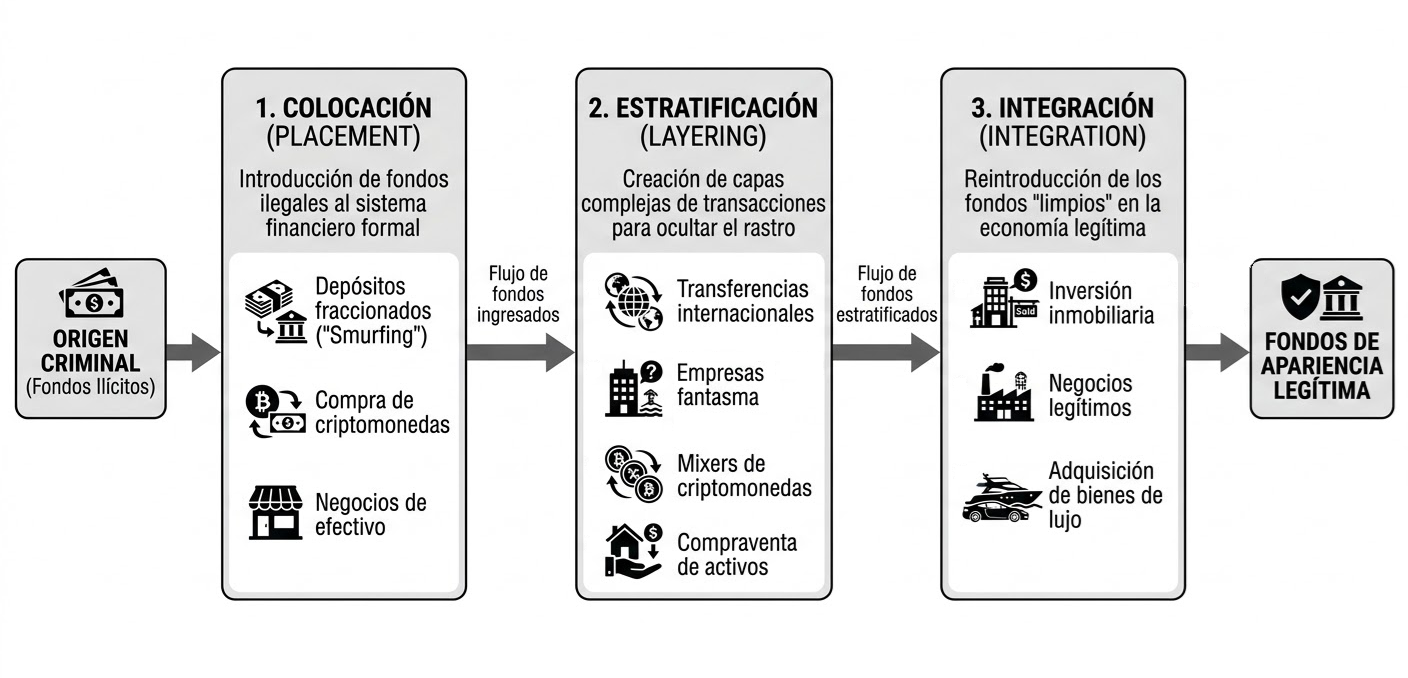
\includegraphics[width=1\textwidth]{chapter_2/images_ch2/money_laundering.png}
    \caption{Diagrama de flujo que ilustra las tres etapas clásicas del lavado de dinero (Colocación, Estratificación e Integración).}
    \label{fig:etapas_lavado}
\end{figure}

\section{Marco Regulatorio Internacional Anti-Lavado de Activos}

\subsection{El Grupo de Acción Financiera Internacional (GAFI/FATF)}

El Grupo de Acción Financiera Internacional (GAFI), conocido en inglés como \textit{Financial Action Task Force} (FATF), constituye la máxima autoridad intergubernamental a nivel mundial en la lucha contra el lavado de activos y el financiamiento del terrorismo. Fundado en 1989 por el G-7, el GAFI está conformado actualmente por 39 países miembros y ha establecido los estándares globales que rigen las políticas de prevención y detección de lavado de activos en todo el mundo \cite{FATF2012InternationalRecommendations}.

El instrumento normativo central del GAFI son las 40 Recomendaciones, un conjunto de medidas financieras, legales y de conducta que los países deben implementar para establecer sistemas efectivos de detección, prevención y represión del lavado de activos y el financiamiento del terrorismo (LA/FT). Estas recomendaciones incluyen disposiciones sobre: evaluación de riesgos, cooperación nacional, tipificación del delito, medidas de decomiso, debida diligencia del cliente (\textit{Customer Due Diligence}, CDD), registro y reporte de operaciones sospechosas, y cooperación internacional.

\subsection{Regulación de activos virtuales y la Regla de Viaje}

Con el crecimiento exponencial de las criptomonedas y los activos virtuales, el GAFI ha actualizado sus directrices para incluir a los Proveedores de Servicios de Activos Virtuales (\textit{Virtual Asset Service Providers}, VASPs) bajo el mismo marco regulatorio que las instituciones financieras tradicionales. 

Un componente clave de esta regulación es la denominada ``Regla de Viaje'' (\textit{Travel Rule}), que exige a los VASPs recopilar y transmitir datos personales tanto del emisor como del receptor para transferencias que superen los 1.000 dólares o euros. Esta disposición busca replicar en el ecosistema cripto los controles de transparencia que ya existen en las transferencias bancarias internacionales, aunque su implementación efectiva sigue siendo un desafío debido a la naturaleza descentralizada de muchas plataformas.

\subsection{Enfoque de Gestión de Riesgos del Comité de Basilea}

A nivel de supervisión bancaria prudencial, el Comité de Basilea para la Supervisión Bancaria (\textit{Basel Committee on Banking Supervision}) emitió directrices sobre la gestión sólida de riesgos relacionados con el lavado de dinero y el financiamiento del terrorismo \cite{BaselCommitteeonBankingSupervision2020SoundTerrorism}. Estas directrices establecen que los bancos deben implementar políticas y procesos robustos para mantener altos estándares éticos y prevenir el uso indebido de sus servicios para actividades criminales.

\subsection{Debida Diligencia del Cliente (KYC)}

En el centro de los marcos regulatorios AML se encuentran los procedimientos de \textit{Know Your Customer} (KYC), que constituyen el componente operativo fundamental para la verificación de identidad de los clientes y la evaluación de sus perfiles de riesgo. Los requisitos de KYC incluyen: la Debida Diligencia del Cliente (CDD) y la Debida Diligencia Reforzada (\textit{Enhanced Due Diligence}, EDD) para clientes de alto riesgo, como personas políticamente expuestas (PEPs) o clientes de jurisdicciones de alto riesgo.

\subsection{El Enfoque Basado en Riesgo}

Los estándares internacionales en materia de prevención del lavado de dinero han desplazado su recomendación desde un modelo de cumplimiento basado en reglas fijas hacia un modelo articulado alrededor del riesgo \cite{FATF2012InternationalRecommendations, BaselCommitteeonBankingSupervision2020SoundTerrorism}. Bajo este principio, conocido como enfoque basado en riesgo, cada institución financiera debe evaluar de manera continua la exposición que representan sus clientes, sus productos, sus canales de distribución y las jurisdicciones con las que opera. A partir de esa evaluación, la institución asigna sus recursos de vigilancia de forma proporcional, de modo que las relaciones de mayor riesgo reciben controles reforzados mientras que las de menor riesgo se someten a medidas simplificadas. De esta manera, el esfuerzo de cumplimiento deja de distribuirse de forma homogénea y pasa a concentrarse donde la amenaza es más plausible.

La lógica que sustenta este enfoque descansa en la eficiencia y en la efectividad del sistema de control en su conjunto. Un régimen de reglas rígidas, que exige el mismo procedimiento a todos los clientes con independencia de su perfil, tiende a saturar a los equipos de cumplimiento con revisiones de bajo valor y a generar un volumen elevado de alertas poco informativas. En contraste, al graduar la intensidad de los controles según el riesgo, la institución libera capacidad analítica para dedicarla a los casos que verdaderamente la ameritan y mejora su probabilidad de detectar operaciones sospechosas. Además, este esquema reconoce que la actividad delictiva evoluciona, por lo que ofrece la flexibilidad necesaria para reasignar recursos cuando aparecen nuevas amenazas sin necesidad de reformar por completo el marco normativo.

Sin embargo, la aplicación práctica del enfoque basado en riesgo plantea desafíos considerables que no deben subestimarse. En primer lugar, la calidad de todo el sistema depende de la solidez de la evaluación de riesgo inicial, la cual exige información confiable, criterios coherentes y personal capacitado para interpretarla, condiciones que no siempre concurren. En segundo lugar, la discrecionalidad que otorga este modelo puede convertirse en una vía para relajar controles de forma indebida, ya sea por presiones comerciales o por una lectura interesada del riesgo, lo que obliga a las autoridades a supervisar cómo se ejerce ese juicio. Por último, la naturaleza cambiante de los productos financieros, y en particular la irrupción de nuevos instrumentos digitales, dificulta clasificar el riesgo de manera estable, de modo que la evaluación requiere una actualización permanente para no quedar desfasada.

\subsection{Desafíos de la Cooperación Transfronteriza}

El lavado de dinero constituye, por su propia naturaleza, un fenómeno que desborda las fronteras de una sola jurisdicción y se despliega a través de múltiples países. Los flujos ilícitos suelen fragmentarse y desplazarse entre distintos sistemas financieros precisamente para dificultar su rastreo y para diluir el vínculo con el delito que los origina. Cuando el circuito de ocultamiento involucra criptomonedas, esta dimensión transnacional se acentúa todavía más, dado que las redes de activos virtuales operan sobre infraestructuras globales que no reconocen los límites políticos tradicionales. En consecuencia, una investigación que se limite al territorio de un solo Estado difícilmente logra reconstruir la totalidad de la cadena de transacciones.

Frente a este carácter global, la respuesta institucional permanece anclada en gran medida a la soberanía de cada país, lo que genera fricciones importantes para la cooperación. El intercambio de información entre autoridades de distintas naciones tropieza con procedimientos formales lentos, con requisitos legales heterogéneos y con celos legítimos en torno a la protección de datos y la confidencialidad. A ello se suma que los marcos legales difieren en la manera de tipificar los delitos, en las facultades que otorgan a los organismos de supervisión y en el grado de exigencia de sus controles preventivos. Estas divergencias hacen que una operación considerada sospechosa en un país pueda pasar inadvertida en otro, y que la evidencia recolectada en una jurisdicción no siempre resulte admisible o útil en la siguiente.

Los actores dedicados al lavado de dinero conocen bien estas asimetrías y las explotan de manera deliberada mediante una práctica que suele denominarse arbitraje regulatorio. En esencia, dirigen sus operaciones hacia aquellas jurisdicciones cuyos controles resultan más débiles, cuya supervisión es más laxa o cuya cooperación internacional es más limitada, con el fin de aprovechar los eslabones más frágiles de la cadena global. De este modo, un sistema de control es tan fuerte como lo permita su componente más permisivo, y los esfuerzos rigurosos de una jurisdicción pueden verse neutralizados por la existencia de refugios normativos en otra. Por esta razón, la comunidad internacional ha insistido en la armonización de estándares y en el fortalecimiento de los mecanismos de asistencia mutua, aun cuando el avance en esa dirección continúe siendo desigual y lento.

\subsection{Proveedores de Servicios de Activos Virtuales y sus Obligaciones}

Los denominados Proveedores de Servicios de Activos Virtuales (\textit{Virtual Asset Service Providers}, VASP) constituyen las entidades que ofrecen servicios de intercambio, custodia, transferencia o administración de criptoactivos por cuenta de terceros. Dentro de esta categoría se ubican, de forma destacada, los \textit{exchanges} de criptomonedas, es decir, las plataformas que permiten convertir moneda tradicional en activos virtuales y viceversa, así como intercambiar unos criptoactivos por otros. Estos proveedores ocupan una posición estratégica en el ecosistema, pues actúan como puntos de conexión entre la economía tradicional y las redes descentralizadas. Justamente por concentrar ese tránsito, se han convertido en un eslabón crítico tanto para el funcionamiento legítimo del sector como para los intentos de canalizar fondos de origen ilícito.

Consciente de esta relevancia, la regulación reciente ha incorporado a los VASP dentro del perímetro de cumplimiento en materia de prevención del lavado de dinero, sujetándolos a obligaciones análogas a las que tradicionalmente han recaído sobre los bancos. Entre esas obligaciones figuran la identificación y verificación de la identidad de sus usuarios, conocida por sus siglas en inglés como \textit{Know Your Customer} (KYC), el monitoreo continuo de las operaciones y el reporte de aquellas que resulten sospechosas ante las autoridades competentes. A ello se añade el deber de transmitir los datos que identifican al emisor y al receptor de una transferencia de activos virtuales, un requisito que replica la lógica de la información que acompaña a las transferencias bancarias convencionales \cite{FATF2012InternationalRecommendations}. Con estas exigencias, los organismos internacionales buscan cerrar la brecha que durante un tiempo permitió que el sector cripto operara al margen de los controles aplicables al resto del sistema financiero.

No obstante, trasladar estas obligaciones a un entorno descentralizado y seudónimo genera retos que carecen de equivalente directo en la banca tradicional. La debida diligencia sobre el cliente se complica cuando las direcciones que operan en una red pública no revelan por sí mismas la identidad de las personas que están detrás de ellas, de modo que un mismo actor puede controlar numerosas direcciones sin exponer un vínculo evidente. La transmisión de los datos del emisor y del receptor resulta particularmente ardua cuando una transferencia involucra billeteras autocustodiadas o proveedores situados en jurisdicciones que no imponen requisitos equivalentes, lo que fragmenta la trazabilidad de la operación. Por añadidura, la velocidad con que surgen nuevos servicios y arreglos técnicos dentro del ecosistema tiende a superar la capacidad de los proveedores para ajustar sus controles, de manera que el cumplimiento efectivo exige un esfuerzo de adaptación constante y recursos analíticos considerables.

\subsection{La Brecha entre Regulación y Capacidad Tecnológica}

Existe una tensión persistente entre el ritmo acelerado con que innova el ecosistema de las criptomonedas y la velocidad, mucho más pausada, con que las instituciones y los reguladores logran adaptar sus herramientas de detección. El sector de los activos virtuales evoluciona de forma vertiginosa, con la aparición continua de nuevos productos, protocolos y formas de intermediación que reconfiguran la manera en que circula el valor. Los marcos normativos, en cambio, requieren procesos deliberativos extensos y ciclos de reforma que difícilmente pueden seguir ese ritmo. Como resultado, cuando una norma o un control finalmente entra en vigor, las prácticas que pretendía atender ya han mutado o han sido reemplazadas por otras.

Esta asimetría se manifiesta con especial claridad en las herramientas de detección que las instituciones emplean para vigilar sus operaciones. Los sistemas tradicionales suelen apoyarse en reglas fijas y umbrales predefinidos que disparan alertas cuando una transacción cumple ciertas condiciones establecidas de antemano. Ese diseño resulta razonable frente a comportamientos conocidos, pero pierde eficacia ante tipologías nuevas que no fueron previstas al momento de formular las reglas, pues quienes buscan ocultar fondos ajustan deliberadamente sus movimientos para permanecer por debajo de los criterios de alerta. Además, un esquema de reglas rígidas tiende a producir una elevada proporción de alertas que finalmente resultan infundadas, lo que satura a los equipos de análisis y desvía su atención de los casos verdaderamente relevantes.

Ante estas limitaciones, el campo de la prevención ha comenzado a explorar enfoques de detección más sofisticados que aspiran a superar la lógica de las reglas fijas. Buena parte del interés se ha orientado hacia métodos capaces de aprovechar la estructura relacional de las transacciones, es decir, la red de vínculos que se forma cuando el dinero se desplaza de un participante a otro y que revela patrones de conexión que un examen aislado de cada operación no alcanza a captar. La intuición que motiva esta dirección sostiene que el comportamiento ilícito rara vez se agota en una transacción individual y, en cambio, deja huellas en la forma en que se organizan los flujos entre múltiples actores. En este trabajo se retoma esa intuición como punto de partida, sin adentrarse por ahora en los detalles técnicos de tales enfoques, que se desarrollan en capítulos posteriores.


\section{Sistemas Tradicionales de Monitoreo de Transacciones}

\subsection{Arquitectura de los sistemas basados en reglas}

Los Sistemas de Monitoreo de Transacciones (\textit{Transaction Monitoring Systems}, TMS) convencionales constituyen la columna vertebral tecnológica del cumplimiento AML en las instituciones financieras desde hace décadas. Estos sistemas se fundamentan en reglas deterministas, listas de vigilancia y umbrales estáticos predefinidos para identificar transacciones potencialmente sospechosas. Su lógica operativa se basa en criterios preestablecidos derivados de patrones conocidos de fraude, tales como cambios súbitos en el volumen de transacciones, ubicaciones geográficas inusuales para compras, o transacciones repetitivas dentro de períodos cortos de tiempo.

\subsection{El problema de los falsos positivos}

El problema más crítico y ampliamente documentado de los TMS convencionales es su extraordinaria tasa de falsos positivos. Según informes de la industria, entre el 90\,\% y el 98\,\% de todas las alertas generadas por los sistemas de monitoreo de transacciones corresponden a falsos positivos \cite{ForresterConsulting2023True2023}. Esto significa que la abrumadora mayoría de las alertas generadas por estos sistemas no corresponden a actividades genuinamente sospechosas, sino a transacciones legítimas.

Las consecuencias operativas de esta tasa son profundas. La carga real puede ascender hasta 22 horas por alerta cuando se consideran los procesos completos de investigación y documentación. Esta sobrecarga genera fatiga organizacional en los equipos de cumplimiento, quienes deben dedicar la mayor parte de su tiempo a perseguir señales falsas en lugar de concentrarse en amenazas genuinas.

\subsection{Costos del cumplimiento AML}

La ineficiencia de los sistemas de monitoreo se traduce directamente en costos económicos desproporcionados. El informe anual \textit{True Cost of Financial Crime Compliance} de 2023 revela que las instituciones financieras a nivel global soportan un costo total de 206.100 millones de dólares por el cumplimiento de delitos financieros \cite{ForresterConsulting2023True2023}. 

Estas cifras ilustran una paradoja fundamental: a pesar de la inversión masiva en sistemas de cumplimiento, el volumen de lavado de activos a nivel global no muestra señales claras de disminución. Como observa Kelkar (2024), los flujos financieros ilícitos continúan representando una amenaza significativa para la estabilidad económica internacional \cite{Kelkar2024AddressingStability}.

\subsection{Consecuencias Operativas y Estratégicas de la Ineficiencia}

La elevada tasa de falsos positivos no es solo un problema de costos, sino que altera la propia lógica de la función de cumplimiento. Cuando la mayor parte del tiempo de los analistas se dedica a descartar alertas irrelevantes, la capacidad de investigación se erosiona y la atención se desplaza desde los casos verdaderamente relevantes hacia un flujo constante de señales espurias. Esta saturación produce un efecto paradójico, ya que un sistema que genera demasiadas alertas incorrectas no solo falla por exceso, sino también por omisión, al aumentar la probabilidad de que operaciones ilícitas genuinas pasen desapercibidas dentro del volumen general de actividad. La ineficiencia, por tanto, compromete de forma simultánea la eficiencia económica y la eficacia detectora del sistema.

A esta dimensión operativa se suma una consecuencia estratégica que rara vez se cuantifica. La fatiga que genera el volumen de falsos positivos deteriora la moral y la retención de los equipos especializados, cuya formación es costosa y cuya experiencia es difícil de reemplazar. En un entorno donde las tipologías de lavado evolucionan con rapidez, la pérdida de talento investigativo reduce la capacidad de la institución para adaptarse a nuevas modalidades de riesgo. Por estas razones, cualquier avance que permita reducir el ruido operativo y dirigir mejor la atención analítica tiene un valor que trasciende el ahorro directo de costos, y se traduce en una mayor resiliencia del sistema de cumplimiento en su conjunto. La Figura \ref{fig:tms_vs_grafos} contrasta el monitoreo basado en reglas con el enfoque relacional basado en grafos que motiva este trabajo.

\begin{figure}[htbp]
    \centering
    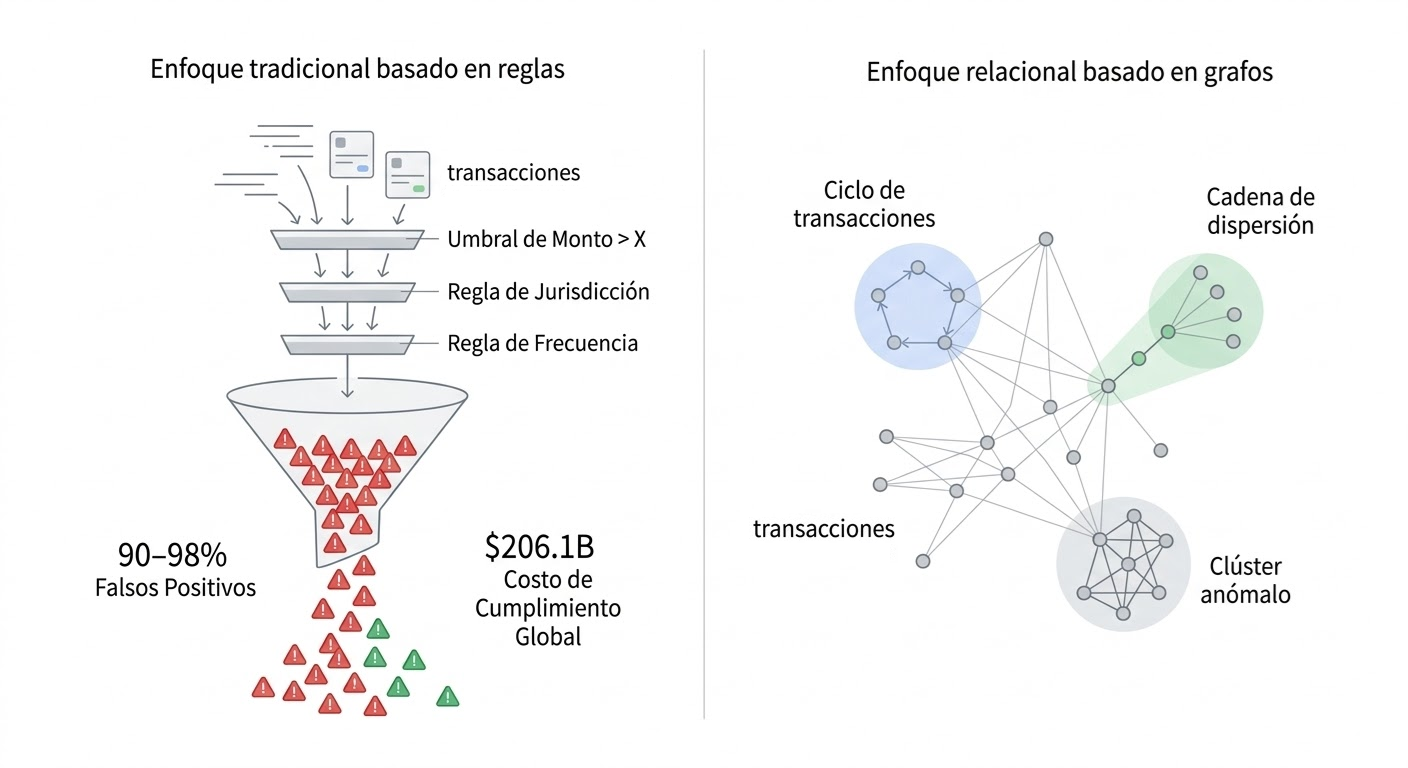
\includegraphics[width=0.9\textwidth]{chapter_2/images_ch2/enfoques_moeny_laundering.png}
    \caption{Comparación entre monitoreo transaccional basado en reglas, con umbrales estáticos y hasta 90-98\% de falsos positivos, y un enfoque relacional basado en grafos, donde las transacciones se analizan como redes para detectar patrones estructurales sospechosos (ciclos, cadenas y vecindarios anómalos).}
    \label{fig:tms_vs_grafos}
\end{figure}

\section{Criptomonedas y Delincuencia Financiera}

\subsection{Seudonimato y arquitectura descentralizada}

La emergencia de las criptomonedas ha transformado radicalmente el panorama del lavado de activos al introducir un medio de transferencia de valor que opera fuera de la infraestructura financiera tradicional \cite{Spotlight2021Cryptocurrencies:Finances}. Es importante realizar una distinción conceptual entre anonimato y seudonimato. Las criptomonedas como Bitcoin no proporcionan anonimato completo, sino seudonimato: cada transacción queda registrada de forma inmutable en la cadena de bloques y es públicamente verificable, pero las direcciones involucradas no están directamente vinculadas a identidades del mundo real \cite{Subashi2024CryptocurrenciesLaundering}.

\subsection{Magnitud de la actividad ilícita en criptomonedas}

Los datos más recientes revelan la magnitud creciente de la actividad criminal en el ecosistema cripto. Según reportes de la industria, en 2025 el volumen ilícito en criptomonedas alcanzó los 154.000 millones de dólares, un aumento sustancial respecto a años anteriores \cite{Chainalysis2025TheReport}. Como señala Europol en su informe EU-SOCTA 2025, la explotación criminal de las criptomonedas ha trascendido el ámbito del cibercrimen para permear áreas delictivas más tradicionales como el narcotráfico y el tráfico de personas \cite{Europol2025EU2025}.

\section{Tipologías de Lavado de Dinero en Criptomonedas}

\subsection{Mezcladores y servicios de ofuscación}

Los \textit{mixers} o \textit{tumblers} de criptomonedas representan una de las herramientas más utilizadas para la estratificación de fondos ilícitos. Funcionan como contratos inteligentes o servicios centralizados que reciben criptomonedas de múltiples usuarios, las combinan en un fondo común, y luego redistribuyen cantidades equivalentes a los participantes, rompiendo así el vínculo rastreable entre las direcciones de origen y destino.

\subsection{Cadenas de pelado (\textit{Peel Chains})}

Las \textit{peel chains} constituyen una técnica de lavado en la que una dirección con una cantidad significativa de criptomonedas realiza transacciones sucesivas, ``pelando'' cantidades cada vez más pequeñas hacia diferentes direcciones en cada paso. Esto distribuye los fondos gradualmente a través de una cadena de direcciones intermedias, creando una estructura transaccional larga y ramificada que complica significativamente el rastreo.

\subsection{Saltos de cadena y puentes entre \textit{blockchains}}

El \textit{chain hopping} o salto de cadena implica la conversión rápida y sucesiva de una criptomoneda a otra, generalmente utilizando diferentes \textit{blockchains}, con el propósito de dificultar el seguimiento de los fondos. Los puentes entre cadenas (\textit{cross-chain bridges}) son las herramientas tecnológicas que facilitan estas transferencias interoperables.

\subsection{Otras técnicas de lavado en criptomonedas}

Además de las técnicas principales, el \textit{smurfing} consiste en fragmentar grandes cantidades en múltiples transacciones pequeñas que quedan por debajo de los umbrales de reporte. Los \textit{exchanges} descentralizados (DEX) y las \textit{privacy coins} como Monero también incorporan protocolos que ofrecen un anonimato estructural superior. Almeida et al. (2025) documentan cómo estas estrategias de dispersión y transacciones encadenadas aprovechan la estructura de red de los ecosistemas digitales \cite{Almeida2025FromTechniques}.

La sofisticación de estas técnicas plantea un desafío directo para los sistemas de detección. Cada nueva modalidad, desde los mezcladores hasta los puentes entre cadenas, añade una capa de ofuscación que rompe la trazabilidad lineal entre el origen y el destino de los fondos. Lo que estas técnicas tienen en común es que su firma no reside en una transacción individual, sino en la configuración de relaciones que forman a través de la red, lo que refuerza la pertinencia de un enfoque estructural para su detección. Un sistema que analice cada transacción de forma aislada difícilmente distinguirá una cadena de pelado de una secuencia de pagos legítimos, mientras que un modelo que observe la topología de la red puede reconocer el patrón característico de fragmentación y dispersión que la define.

\subsection{Comparación de técnicas de lavado}

La Tabla \ref{tecnicas_lavado} sintetiza las principales técnicas de lavado de dinero empleadas en el ecosistema de criptomonedas.

\begin{table}[t]
    \centering
    \renewcommand{\arraystretch}{1.3}
    \begin{tabular}{|p{3.5cm}|p{2.5cm}|p{5.5cm}|p{2.5cm}|}
    \hline
    \textbf{Técnica} & \textbf{Etapa predominante} & \textbf{Mecanismo} & \textbf{Complejidad de detección} \\
    \hline
    \textit{Smurfing} / Estructuración & Colocación & Fraccionamiento de transacciones bajo umbrales de reporte & Media \\
    \hline
    \textit{Mixers} / \textit{Tumblers} & Estratificación & Combinación de fondos de múltiples usuarios para romper trazabilidad & Alta \\
    \hline
    \textit{Peel Chains} & Estratificación & Transferencias sucesivas de montos decrecientes a múltiples direcciones & Alta \\
    \hline
    \textit{Chain Hopping} & Estratificación & Conversión rápida entre diferentes \textit{blockchains} & Muy alta \\
    \hline
    \textit{Cross-chain Bridges} & Estratificación & Puentes tecnológicos para transferir valor entre \textit{blockchains} distintas & Muy alta \\
    \hline
    \textit{Trading} en DEX & Estratificación & Intercambio directo P2P sin intermediario centralizado & Alta \\
    \hline
    \textit{Privacy Coins} & Estrat./Integ. & Protocolos criptográficos que anonimizan transacciones por diseño & Muy alta \\
    \hline
    Compra de activos & Integración & Adquisición de bienes inmuebles, lujo con cripto convertido & Baja a Media \\
    \hline
    \end{tabular}
    \caption{Principales técnicas de lavado de dinero en criptomonedas}
    \label{tecnicas_lavado}
\end{table}

\section{Desafíos de la Detección de Fraude Financiero en el Ecosistema Cripto}

\subsection{Desafíos operativos y regulatorios}

La detección de lavado de dinero en criptomonedas enfrenta un conjunto interrelacionado de desafíos que trascienden las capacidades de los sistemas convencionales. En primer lugar, el seudonimato inherente a las criptomonedas dificulta la identificación de las partes involucradas. En segundo lugar, la naturaleza transfronteriza genera desafíos jurisdiccionales significativos. En tercer lugar, la velocidad de las transacciones en el ecosistema cripto supera ampliamente la capacidad de respuesta de los mecanismos tradicionales de monitoreo \cite{Subashi2024CryptocurrenciesLaundering}.

\subsection{La brecha entre regulación y realidad operativa}

Existe una tensión inherente entre el ritmo de innovación en el ecosistema cripto y la capacidad de los marcos regulatorios para adaptarse. Este contexto regulatorio fragmentado es particularmente relevante para la presente tesis, ya que subraya la necesidad de desarrollar herramientas de detección que puedan operar de forma efectiva basándose en los patrones estructurales y relacionales que las transacciones exhiben dentro de la red.


\section{Del Monitoreo Basado en Reglas hacia Enfoques Estructurales}

\subsection{Limitaciones fundamentales del enfoque tabular}

La limitación estructural común a los sistemas tradicionales de detección AML es su tratamiento de las transacciones como eventos aislados e independientes. Los TMS convencionales analizan cada transacción en función de sus atributos individuales sin considerar las relaciones topológicas entre las entidades involucradas.

\subsection{Transacciones financieras como grafos}

La representación de redes transaccionales como grafos ofrece un marco conceptual natural para abordar las limitaciones del enfoque tabular. En este paradigma, las entidades financieras se representan como nodos del grafo, mientras que las transacciones entre ellas constituyen las aristas. Esta formulación permite capturar propiedades fundamentales de las redes financieras que son invisibles para los modelos tabulares.

Esta representación relacional habilita un conjunto de análisis que el enfoque tabular no puede realizar. La posición de una transacción dentro de la red, medida por indicadores de centralidad, revela su importancia estructural más allá de sus atributos individuales. Los patrones de conectividad permiten identificar configuraciones características del lavado, como cadenas de intermediación, ciclos de reintegración o estructuras de dispersión en las que un origen reparte fondos hacia numerosos destinos. La propagación de información a través de la red hace posible que la clasificación de una transacción incorpore el contexto de sus vecinos, de modo que una operación individualmente benigna pueda señalarse como sospechosa por la compañía que mantiene dentro del grafo. Estas capacidades explican por qué el modelado basado en grafos se ha consolidado como el enfoque de referencia para la detección estructural de actividad ilícita en criptomonedas.

No obstante, la perspectiva de red introduce también desafíos que el enfoque tabular no enfrenta. La calidad de las conclusiones depende de la calidad de las conexiones observadas, y una red incompleta o ruidosa puede inducir a error tanto al clasificador como a las explicaciones que de él se derivan. La dispersión de la red, es decir la escasez de conexiones por nodo, limita la información contextual disponible y, como se documenta en el Capítulo 4, puede llegar a impedir que las explicaciones estructurales sean informativas. Reconocer estas limitaciones desde el marco contextual es necesario para interpretar con prudencia los resultados que las técnicas basadas en grafos producen, y anticipa la necesidad de un eje experimental complementario que permita evaluar aquello que un grafo disperso no deja medir.

\subsection{El Elliptic Dataset como referente de datos reales}

En el contexto específico de la detección AML en Bitcoin, el \textit{Elliptic Dataset} se ha consolidado como uno de los conjuntos de datos de referencia más importantes. El trabajo pionero de Weber et al. (2019) demostró que la representación de la red de transacciones Bitcoin como un grafo permite capturar patrones estructurales que los modelos tabulares no pueden identificar \cite{Weber2019Anti-MoneyForensics}. Unagar y Borisaniya (2025) confirman que los métodos basados en grafos representan el estado más avanzado de la técnica para este dominio \cite{Unagar2025SurveyXAI}.

\subsection{Hacia la necesidad de modelos explicables}

En un entorno donde las decisiones automatizadas pueden derivar en el bloqueo de cuentas o investigaciones con implicaciones jurídicas significativas, la capacidad de explicar y justificar las alertas generadas es tan importante como su precisión predictiva. Esto implica que los modelos de detección deben producir no solo una clasificación binaria, sino también una justificación comprensible del porqué. Este requisito conecta directamente con el objeto central de la presente tesis: la evaluación de la estabilidad de los métodos de explicabilidad (XAI) aplicados a modelos de grafos para detección AML.

\chapter{FUNDAMENTOS DE IA PARA DETECCIÓN DE FRAUDE FINANCIERO}

El presente capítulo introduce los fundamentos técnicos del Aprendizaje Automático (\textit{Machine Learning}, ML) y el Aprendizaje Profundo (\textit{Deep Learning}, DL) aplicados al dominio de detección de fraude financiero. Se enfatiza particularmente en las \textit{Graph Neural Networks} (GNNs), arquitecturas que representan el estado del arte para el análisis de datos relacionales como las redes transaccionales. El capítulo caracteriza de forma comparativa las cuatro arquitecturas evaluadas en esta tesis, a saber GCN, GraphSAGE, GAT y TAGCN, describe sus mecanismos de agregación y prepara al lector para el diseño experimental de los capítulos posteriores. En lugar de designar una arquitectura ganadora de antemano, el estudio plantea a TAGCN como un caso de interés inicial por su agregación multi-hop, y trata la expectativa de que esa capacidad se traduzca en mejores explicaciones como una hipótesis que los resultados someten a contraste. Además, se introducen las nociones estadísticas que sostienen el análisis posterior, de manera que las afirmaciones sobre estabilidad se acompañen de medidas de incertidumbre en lugar de descansar sobre una única ejecución.

\section{Del Aprendizaje Automático al Aprendizaje Profundo}

\subsection{Aprendizaje Automático: Definición y Paradigmas}

El Aprendizaje Automático constituye un subcampo de la inteligencia artificial orientado al desarrollo de algoritmos capaces de aprender patrones a partir de datos sin ser explícitamente programados para cada tarea específica. En el contexto de detección de fraude financiero, los enfoques de ML han evolucionado desde sistemas basados en reglas deterministas hacia modelos estadísticos que identifican comportamientos anómalos mediante el análisis de características transaccionales.

Los paradigmas fundamentales del ML se clasifican en tres categorías principales:

\begin{itemize}
    \item \textbf{Aprendizaje Supervisado}: El modelo aprende a partir de datos etiquetados, donde cada instancia de entrenamiento está asociada con una etiqueta conocida (por ejemplo, "lícita" o "ilícita"). Este paradigma es fundamental para la detección AML, donde se busca clasificar transacciones en función de ejemplos históricos verificados. Los algoritmos clásicos incluyen regresión logística, árboles de decisión, \textit{Random Forest} y \textit{Support Vector Machines} (SVM) \cite{Unagar2025SurveyXAI}.
    \item \textbf{Aprendizaje No Supervisado}: El modelo identifica estructuras ocultas en datos no etiquetados, siendo particularmente útil para la detección de anomalías cuando no se dispone de suficientes ejemplos etiquetados de fraude. Técnicas como \textit{clustering} (K-means, DBSCAN) y reducción de dimensionalidad (PCA, t-SNE) han sido empleadas para identificar patrones transaccionales atípicos.
    \item \textbf{Aprendizaje Semi-Supervisado}: Combina un pequeño conjunto de datos etiquetados con una gran cantidad de datos sin etiquetar, aprovechando la estructura subyacente de los datos para mejorar el rendimiento del modelo. Este paradigma es especialmente relevante en AML, donde las etiquetas verificadas son costosas de obtener debido a la necesidad de investigación manual \cite{Lawal2025AnDataset}.
\end{itemize}

\subsection{Limitaciones del ML Tabular en Detección AML}

Los métodos tradicionales de ML tratan las transacciones financieras como instancias independientes, representadas mediante vectores de características numéricas extraídas de cada transacción individual: monto, frecuencia, geolocalización, temporalidad, entre otras. Aunque estos enfoques han demostrado capacidad para identificar patrones conocidos de fraude, enfrentan limitaciones estructurales en escenarios contemporáneos de lavado de activos \cite{Unagar2025SurveyXAI}.

La primera limitación radica en su incapacidad para capturar dependencias relacionales. El lavado de dinero no se manifiesta únicamente en las características de una transacción aislada, sino en patrones topológicos que emergen de múltiples transacciones interconectadas: cadenas de dispersión, ciclos transaccionales, estructuras de intermediación artificial y vecindarios sospechosos \cite{Weber2019Anti-MoneyForensics, Lawal2025AnDataset}. Los modelos tabulares, al ignorar estas dependencias, pierden información crítica sobre la estructura de la red financiera.

La segunda limitación es la ingeniería de características manual. Los enfoques clásicos requieren que expertos del dominio diseñen características agregadas que intenten capturar información relacional de forma indirecta (por ejemplo, número de conexiones, promedios de montos de vecinos). Este proceso es laborioso, dependiente del conocimiento experto y potencialmente incompleto frente a tipologías de fraude emergentes \cite{Unagar2025SurveyXAI}.

La tercera limitación concierne a la escalabilidad. A medida que las redes transaccionales crecen en tamaño y complejidad, la construcción manual de características relacionales se vuelve computacionalmente intratable. Este problema es particularmente agudo en ecosistemas de criptomonedas, donde la velocidad y el volumen de transacciones superan ampliamente los flujos financieros tradicionales.

\subsection{El Aprendizaje Profundo como Paradigma de Representación}

El Aprendizaje Profundo representa una evolución del ML caracterizada por el uso de arquitecturas neuronales con múltiples capas de procesamiento que aprenden representaciones jerárquicas de los datos de forma automática. A diferencia de los métodos tradicionales que requieren ingeniería manual de características, los modelos de DL son capaces de descubrir automáticamente representaciones útiles directamente desde los datos crudos \cite{Unagar2025SurveyXAI, He2026AnDetection}.

Las redes neuronales profundas han demostrado capacidad excepcional para modelar funciones complejas no lineales en dominios diversos: visión computacional, procesamiento de lenguaje natural, reconocimiento de voz y, más recientemente, análisis de grafos. Su arquitectura multicapa permite que las capas iniciales capturen características de bajo nivel (patrones simples), mientras que capas superiores construyen representaciones abstractas de alto nivel mediante composición jerárquica.

En el contexto de detección AML, el DL ofrece dos ventajas fundamentales: primero, la capacidad de aprender automáticamente características discriminativas desde datos transaccionales sin requerir conocimiento experto previo; segundo, la flexibilidad arquitectónica para incorporar diferentes tipos de datos (atributos numéricos, secuencias temporales, estructuras de grafos) dentro de un marco unificado \cite{He2026AnDetection}.

No obstante, esta potencia representacional introduce un desafío crítico: la opacidad. Los modelos de DL operan como "cajas negras" cuyo proceso interno de decisión es difícil de interpretar, generando una tensión entre desempeño predictivo y auditabilidad en dominios regulados como AML \cite{Gawantka2024AExplanations}.

Esta tensión entre potencia y opacidad es especialmente aguda en el dominio financiero, donde las decisiones automatizadas están sujetas a escrutinio regulatorio. Un modelo tabular simple, como un árbol de decisión, ofrece una interpretabilidad casi total a costa de una capacidad limitada para capturar patrones complejos, mientras que una red profunda invierte esa relación. El aprendizaje profundo sobre grafos hereda esta tensión y le añade una dificultad propia, la de explicar qué atributos influyen en una predicción y qué relaciones estructurales lo hacen. Esta doble opacidad, sobre features y sobre estructura, es la que motiva el desarrollo de métodos de explicabilidad específicos para grafos, y la que sitúa el estudio de su estabilidad en el centro de la agenda de la IA explicable aplicada a las finanzas.

\section{Graph Neural Networks: Fundamentos Conceptuales}

\subsection{Representación de Datos Financieros como Grafos}

Un grafo $G = (V, E)$ consiste en un conjunto de nodos (vértices) $V$ y un conjunto de aristas (conexiones) $E$ que conectan pares de nodos. En el dominio de transacciones financieras, esta representación es naturalmente adecuada: cada entidad (cuenta bancaria, billetera de criptomonedas, usuario) se modela como un nodo, mientras que cada transacción entre dos entidades constituye una arista dirigida que conecta el nodo origen con el nodo destino \cite{Weber2019Anti-MoneyForensics, Lawal2025AnDataset}.

Formalmente, sea $G = (V, E, \mathbf{X}, \mathbf{y})$ un grafo donde:

\begin{itemize}
    \item $V = \{v_1, v_2, \ldots, v_N\}$ representa el conjunto de $N$ nodos (entidades financieras).
    \item $E \subseteq V \times V$ representa el conjunto de aristas (transacciones).
    \item $\mathbf{X} \in \mathbb{R}^{N \times F}$ es la matriz de características de nodos, donde cada fila $\mathbf{x}_i \in \mathbb{R}^F$ contiene $F$ características del nodo $v_i$.
    \item $\mathbf{y} \in \{0,1\}^N$ es el vector de etiquetas, donde $y_i = 1$ indica actividad ilícita.
\end{itemize}

En el \textit{Elliptic Dataset}, cada nodo representa una transacción de Bitcoin con 166 características que incluyen: estadísticas agregadas del flujo transaccional (número de entradas/salidas, montos totales), características temporales y propiedades topológicas locales. Las aristas conectan transacciones que comparten direcciones Bitcoin, capturando así el flujo de fondos en la red \cite{Weber2019Anti-MoneyForensics, Lawal2025AnDataset}.

Esta formulación gráfica permite expresar explícitamente las dependencias relacionales que los modelos tabulares ignoran. Por ejemplo, una transacción puede ser benigna cuando se analiza aisladamente, pero sospechosa cuando se observa su posición dentro de una cadena de dispersión (\textit{peel chain}) o su proximidad a servicios de mezcla conocidos (\textit{mixers}).

\subsection{El Paradigma de Message Passing}

Las \textit{Graph Neural Networks} operan bajo el principio de \textit{message passing} (paso de mensajes), un marco computacional donde cada nodo actualiza iterativamente su representación mediante la agregación de información de sus vecinos en el grafo \cite{Du2017TopologyNetworks, He2026AnDetection}.

El proceso general de una capa GNN se puede descomponer en tres operaciones fundamentales:

\textbf{1. Generación de Mensajes (Message Function)}: Para cada nodo $v_i$, se generan mensajes desde sus vecinos $\mathcal{N}(v_i)$ usando una función parametrizada:
\[ m_{ji}^{(k)} = \text{MESSAGE}^{(k)}(\mathbf{h}_j^{(k-1)}, \mathbf{h}_i^{(k-1)}, e_{ji}) \]
donde $\mathbf{h}_i^{(k-1)}$ es la representación del nodo $i$ en la capa anterior, $\mathbf{h}_j^{(k-1)}$ es la representación de un vecino $j$, y $e_{ji}$ representa las características de la arista.

\textbf{2. Agregación de Mensajes (Aggregation Function)}: Los mensajes recibidos se combinan mediante una función de agregación invariante a permutaciones (\textit{permutation-invariant}):
\[ \mathbf{m}_i^{(k)} = \text{AGGREGATE}^{(k)} \left( \{m_{ji}^{(k)} : j \in \mathcal{N}(v_i)\} \right) \]
Funciones comunes de agregación incluyen suma ($\sum$), promedio ($\text{mean}$), máximo ($\max$) o funciones más complejas como LSTM.

\textbf{3. Actualización de Estado (Update Function)}: La representación del nodo se actualiza combinando su estado anterior con el mensaje agregado:
\[ \mathbf{h}_i^{(k)} = \text{UPDATE}^{(k)}(\mathbf{h}_i^{(k-1)}, \mathbf{m}_i^{(k)}) \]
Típicamente implementado como: $\mathbf{h}_i^{(k)} = \sigma(\mathbf{W}^{(k)} [\mathbf{h}_i^{(k-1)} \, \| \, \mathbf{m}_i^{(k)}])$, donde $\mathbf{W}^{(k)}$ son parámetros aprendibles, $\|$ denota concatenación y $\sigma$ es una función de activación no lineal (ReLU, tanh).

Este proceso se repite por $K$ capas, permitiendo que cada nodo agregue información desde vecindarios cada vez más amplios. Después de $K$ iteraciones, la representación de un nodo captura información estructural hasta una distancia de $K$ saltos en el grafo.

El número de capas define así el campo receptivo del modelo, es decir el conjunto de nodos que pueden influir en la predicción de un nodo dado. Esta noción es central para la explicabilidad, ya que una explicación estructural solo puede señalar elementos que se encuentren dentro del campo receptivo, y su tamaño depende tanto del número de capas como de la densidad del grafo. En grafos densos, un campo receptivo de dos saltos puede abarcar decenas o cientos de nodos, mientras que en grafos dispersos como el \textit{Elliptic Dataset} ese mismo campo receptivo se reduce a unos pocos nodos, lo que limita de raíz lo que una explicación puede expresar. El aumento del número de capas tampoco es una solución sin costo, puesto que apilar demasiadas capas provoca el fenómeno de sobre-suavizado, en el que las representaciones de nodos distintos convergen y pierden capacidad discriminativa. Estas consideraciones justifican que las arquitecturas de esta tesis empleen un número reducido de capas y que las explicaciones se calculen sobre el campo receptivo real de cada nodo, un punto que el Capítulo 4 desarrolla con detalle.

Un ejemplo concreto ilustra cómo el paso de mensajes captura patrones de lavado. Considérese una cuenta que recibe transferencias de numerosas cuentas de origen y las consolida, una configuración característica de la tipología de recolección. En la primera capa, la representación de la cuenta consolidadora agrega la información de sus vecinos inmediatos, de modo que incorpora la señal de recibir muchos flujos entrantes. En la segunda capa, esa representación ya enriquecida se combina con la de vecinos a dos saltos, lo que permite al modelo reconocer que la cuenta recibe muchos flujos y que esos flujos provienen, a su vez, de estructuras dispersas. De esta manera, dos capas de paso de mensajes bastan para que el modelo distinga una consolidación legítima de una que forma parte de una estructura de recolección más amplia, algo que un modelo tabular, al observar la cuenta de forma aislada, no podría lograr.

\subsection{Ventajas de las GNNs en Detección AML}

Las GNNs ofrecen tres ventajas fundamentales sobre métodos tradicionales en el contexto AML:

\begin{itemize}
    \item \textbf{Captura de Dependencias Estructurales}: Las GNNs explotan explícitamente la topología del grafo, permitiendo identificar patrones relacionales invisibles para modelos tabulares. Por ejemplo, pueden detectar que una transacción forma parte de una cadena de dispersión al analizar el patrón de conectividad de sus vecinos hasta múltiples saltos \cite{Weber2019Anti-MoneyForensics, Lawal2025AnDataset}.
    \item \textbf{Aprendizaje de Representaciones End-to-End}: Las GNNs aprenden automáticamente representaciones óptimas de nodos mediante \textit{backpropagation}, eliminando la necesidad de ingeniería manual de características relacionales. Las representaciones aprendidas codifican tanto atributos intrínsecos de los nodos como su posición estructural en la red \cite{Du2017TopologyNetworks, He2026AnDetection}.
    \item \textbf{Capacidad Inductiva}: Arquitecturas como GraphSAGE y GAT son inductivas, es decir, pueden generar representaciones para nodos nunca vistos durante el entrenamiento mediante la aplicación de funciones de agregación aprendidas. Esta propiedad es crítica en redes financieras dinámicas donde continuamente emergen nuevas entidades y transacciones.
\end{itemize}

Diversos estudios recientes reportan la ventaja de las GNNs en detección AML de forma verificada mediante experimentos controlados. Lawal et al. mostraron que los modelos basados en grafos superan de manera consistente a los enfoques tabulares en el \textit{Elliptic Dataset} \cite{Lawal2025AnDataset}. He et al. describieron un marco explicable en el que las GNNs capturan patrones estructurales que los métodos tabulares no logran recuperar \cite{He2026AnDetection}. Conviene matizar que esta ventaja no es incondicional, ya que su magnitud depende de la densidad del grafo, de la calidad de las conexiones observadas y de la arquitectura concreta empleada, un punto que los resultados de esta tesis abordan de manera directa.

\section{Arquitecturas GNN Fundamentales}

\subsection{Graph Convolutional Networks (GCN)}

Las \textit{Graph Convolutional Networks}, propuestas por Kipf y Welling, constituyen una de las arquitecturas GNN más influyentes. Su diseño simplifica la convolución espectral en grafos mediante una formulación espacial eficiente \cite{Kipf2017Semi-SupervisedNetworks}.

La regla de propagación de una capa GCN se define como:
\[ \mathbf{H}^{(k+1)} = \sigma(\tilde{\mathbf{D}}^{-1/2} \tilde{\mathbf{A}} \tilde{\mathbf{D}}^{-1/2} \mathbf{H}^{(k)} \mathbf{W}^{(k)}) \]
donde:
\begin{itemize}
    \item $\mathbf{H}^{(k)} \in \mathbb{R}^{N \times F_k}$ es la matriz de representaciones de nodos en la capa $k$.
    \item $\tilde{\mathbf{A}} = \mathbf{A} + \mathbf{I}$ es la matriz de adyacencia con \textit{self-loops} agregados.
    \item $\tilde{\mathbf{D}}$ es la matriz diagonal de grados correspondiente a $\tilde{\mathbf{A}}$.
    \item $\mathbf{W}^{(k)} \in \mathbb{R}^{F_k \times F_{k+1}}$ son parámetros aprendibles.
    \item $\sigma$ es una función de activación no lineal.
\end{itemize}

Esta formulación realiza un promedio ponderado normalizado de las características de los vecinos, seguido de una transformación lineal y activación no lineal. La normalización simétrica $\tilde{\mathbf{D}}^{-1/2} \tilde{\mathbf{A}} \tilde{\mathbf{D}}^{-1/2}$ estabiliza el entrenamiento al prevenir que nodos con muchos vecinos dominen la agregación.

\textbf{Características principales de GCN}:
\begin{itemize}
    \item \textbf{Agregación isotrópica}: Todos los vecinos contribuyen igualmente (solo ponderados por grado).
    \item \textbf{Eficiencia computacional}: Operación matricial dispersa eficiente.
    \item \textbf{Aprendizaje transductivo}: Diseñado originalmente para clasificación en grafos estáticos completos.
    \item \textbf{Limitación}: Tratamiento uniforme de vecinos puede ser subóptimo cuando diferentes vecinos tienen relevancia distinta para la tarea.
\end{itemize}

Weber et al. demostraron que GCN aplicada al \textit{Elliptic Dataset} supera significativamente a modelos tabulares clásicos, capturando patrones estructurales de lavado de dinero \cite{Weber2019Anti-MoneyForensics}.

\subsection{GraphSAGE: Aprendizaje Inductivo y Muestreo de Vecindarios}

GraphSAGE (\textit{Graph Sample and AggregatE}), propuesta por Hamilton, Ying y Leskovec, introduce dos innovaciones fundamentales: capacidad inductiva mediante funciones de agregación aprendidas y escalabilidad mediante muestreo de vecindarios \cite{Hamilton2017InductiveGraphs}.

La actualización de representación en GraphSAGE se formula como:
\[ \mathbf{h}_i^{(k)} = \sigma(\mathbf{W}^{(k)} \cdot \text{CONCAT}(\mathbf{h}_i^{(k-1)}, \text{AGG}^{(k)}(\{\mathbf{h}_j^{(k-1)}, \forall j \in \mathcal{N}(v_i)\}))) \]
donde AGG puede ser:
\begin{itemize}
    \item \textbf{Mean aggregator}: $\text{AGG} = \frac{1}{|\mathcal{N}(v_i)|} \sum_{j \in \mathcal{N}(v_i)} \mathbf{h}_j^{(k-1)}$
    \item \textbf{Max aggregator}: $\text{AGG} = \max(\{\sigma(\mathbf{W} \mathbf{h}_j^{(k-1)} + \mathbf{b}), \forall j \in \mathcal{N}(v_i)\})$
    \item \textbf{LSTM aggregator}: Aplicación de LSTM sobre permutación aleatoria de vecinos.
\end{itemize}

\textbf{Muestreo de vecindarios}: Para mantener complejidad computacional constante, GraphSAGE muestrea un número fijo $S$ de vecinos en cada capa. Esto previene la explosión exponencial del árbol de computación y permite entrenamiento por \textit{mini-batches}.

\textbf{Características principales}:
\begin{itemize}
    \item \textbf{Aprendizaje inductivo}: Generaliza a nodos no vistos durante entrenamiento.
    \item \textbf{Escalabilidad}: Muestreo controla complejidad computacional.
    \item \textbf{Flexibilidad}: Diferentes agregadores capturan diferentes patrones relacionales.
    \item \textbf{Aplicabilidad AML}: Crítico para redes transaccionales dinámicas donde continuamente emergen nuevas entidades.
\end{itemize}

\subsection{Graph Attention Networks (GAT)}

Las \textit{Graph Attention Networks}, introducidas por Velickovic et al., incorporan mecanismos de atención que permiten asignar pesos aprendibles a diferentes vecinos, superando la limitación isotrópica de GCN \cite{Velickovic2018GraphNetworks}.

El mecanismo de atención en GAT se define como:
\[ \alpha_{ij} = \frac{\exp(\text{LeakyReLU}(\mathbf{a}^T[\mathbf{W}\mathbf{h}_i \, \| \, \mathbf{W}\mathbf{h}_j]))}{\sum_{k \in \mathcal{N}(v_i)} \exp(\text{LeakyReLU}(\mathbf{a}^T[\mathbf{W}\mathbf{h}_i \, \| \, \mathbf{W}\mathbf{h}_k]))} \]
Los coeficientes de atención $\alpha_{ij}$ determinan la importancia del vecino $j$ para el nodo $i$. La actualización de representación es entonces:
\[ \mathbf{h}_i^{(k)} = \sigma \left( \sum_{j \in \mathcal{N}(v_i)} \alpha_{ij}^{(k)} \mathbf{W}^{(k)} \mathbf{h}_j^{(k-1)} \right) \]

\textbf{Multi-head attention}: GAT emplea múltiples cabezas de atención en paralelo, concatenando o promediando sus salidas para estabilizar el aprendizaje y capturar diferentes aspectos relacionales.

\textbf{Características principales}:
\begin{itemize}
    \item \textbf{Agregación anisotrópica}: Diferentes vecinos reciben pesos distintos según relevancia aprendida.
    \item \textbf{Interpretabilidad parcial}: Los coeficientes de atención pueden inspeccionarse.
    \item \textbf{Capacidad expresiva}: Superior a GCN en tareas donde la importancia de vecinos varía.
    \item \textbf{Costo computacional}: Mayor complejidad que GCN debido a cálculo de atención por arista.
\end{itemize}

Xu et al. mostraron que mecanismos de atención mejoran la detección AML al ponderar selectivamente conexiones sospechosas en la red transaccional \cite{Lin2026DetectingLaundering}.

\section{TAGCN: Agregación Multi-Hop mediante Filtros Polinomiales}

\subsection{Motivación y Fundamento Teórico}

La \textit{Topology Adaptive Graph Convolutional Network} (TAGCN) constituye una extensión de las GNNs convencionales que incorpora filtros polinomiales adaptativos para capturar dependencias estructurales de mayor alcance \cite{Du2017TopologyNetworks}. A diferencia de GCN, que emplea una aproximación de primer orden (vecindario inmediato), TAGCN define filtros que pueden agregar información desde múltiples saltos topológicos mediante polinomios de Chebyshev.

La formulación de TAGCN se basa en la teoría de procesamiento de señales en grafos (\textit{Graph Signal Processing}, GSP), donde las convoluciones espectrales en grafos se pueden expresar como filtros polinomiales sobre la matriz de adyacencia normalizada:
\[ g_\theta(\mathbf{L}) = \sum_{k=0}^{K-1} \theta_k \mathbf{T}_k(\tilde{\mathbf{L}}) \]
donde:
\begin{itemize}
    \item $\mathbf{L}$ es el Laplaciano normalizado del grafo.
    \item $\tilde{\mathbf{L}} = 2\mathbf{L}/\lambda_{\max} - \mathbf{I}$ es el Laplaciano reescalado al intervalo $[-1, 1]$.
    \item $\mathbf{T}_k$ son polinomios de Chebyshev de orden $k$.
    \item $\theta_k$ son parámetros aprendibles.
\end{itemize}

La recursión de Chebyshev permite computar eficientemente los polinomios sin calcular la descomposición espectral completa del grafo:
\[ \mathbf{T}_0(\mathbf{x}) = 1, \quad \mathbf{T}_1(\mathbf{x}) = \mathbf{x}, \quad \mathbf{T}_k(\mathbf{x}) = 2\mathbf{x}\mathbf{T}_{k-1}(\mathbf{x}) - \mathbf{T}_{k-2}(\mathbf{x}) \]

En la práctica, TAGCN típicamente utiliza $K=3$, limitándose a polinomios de segundo grado para mantener simplicidad computacional mientras captura dependencias hasta 2 saltos en el grafo \cite{Du2017TopologyNetworks}.

La formulación polinomial de TAGCN se sitúa en la frontera entre los enfoques espectrales y espaciales del aprendizaje sobre grafos. Los métodos espectrales definen la convolución en el dominio de la frecuencia del grafo, a través de la descomposición del Laplaciano, lo que ofrece una fundamentación teórica sólida pero un costo computacional elevado y una dependencia de la estructura global. Los métodos espaciales, en cambio, definen la agregación directamente sobre los vecindarios, lo que resulta más eficiente y flexible pero menos fundamentado en la teoría de señales. Al aproximar el filtro espectral mediante polinomios de la matriz de adyacencia, TAGCN conserva parte del rigor de los métodos espectrales mientras opera con la eficiencia de los espaciales, lo que explica el interés inicial que despertó como candidato para grafos financieros de gran tamaño.

\subsection{Ventajas de TAGCN para Detección AML}

TAGCN ofrece varias ventajas específicas para el dominio de detección de lavado de dinero:

\begin{itemize}
    \item \textbf{Captura de Patrones Multi-Hop}: Las tipologías de lavado frecuentemente involucran cadenas de transacciones intermediarias (\textit{peel chains, chain hopping}) que se extienden más allá del vecindario inmediato. TAGCN puede capturar estos patrones mediante filtros de orden superior que agregan información desde múltiples saltos topológicos \cite{Du2017TopologyNetworks}.
    \item \textbf{Adaptabilidad Topológica}: Los filtros polinomiales se adaptan automáticamente a la topología local del grafo. En regiones densamente conectadas, el filtro captura información de muchos nodos; en regiones dispersas, se enfoca en conexiones más lejanas. Esta adaptabilidad es valiosa en redes financieras heterogéneas.
    \item \textbf{Fundamentación Teórica Sólida}: A diferencia de aproximaciones heurísticas, TAGCN está fundamentada en teoría de procesamiento de señales en grafos, garantizando propiedades deseables como invariancia a permutaciones y consistencia con definiciones clásicas de convolución.
    \item \textbf{Eficiencia Computacional}: Al limitarse a polinomios de grado bajo (típicamente $K=3$), TAGCN mantiene complejidad lineal en el número de aristas, siendo más eficiente que métodos que requieren agregación desde vecindarios extensos.
    \item \textbf{Rendimiento reportado en la literatura}: Du et al. reportaron que TAGCN obtiene resultados competitivos en varios \textit{benchmarks} de clasificación de nodos \cite{Du2017TopologyNetworks}. Esos resultados provienen de grafos de citación académica, de modo que su traslado al dominio AML y a la estabilidad de las explicaciones constituye una cuestión abierta que esta tesis examina en lugar de asumir.
\end{itemize}

\subsection{Implementación y Hiperparámetros de TAGCN}

La arquitectura TAGCN empleada en esta investigación sigue la formulación estándar con configuraciones específicas para el dominio AML:

\begin{itemize}
    \item \textbf{Estructura de Capas}: Se emplea una arquitectura de dos capas:
    \begin{itemize}
        \item Primera capa: de las 166 características de entrada a 64 unidades ocultas con ReLU.
        \item Segunda capa: de las 64 unidades ocultas a 2 clases (lícita/ilícita) con softmax.
    \end{itemize}
    \item \textbf{Filtro Polinomial}: Orden $K=3$, capturando dependencias hasta 2 saltos en el grafo.
    \item \textbf{Normalización}: Se emplea normalización simétrica de la matriz de adyacencia:
    \[ \mathbf{A}_{\text{norm}} = \mathbf{D}^{-1/2} \mathbf{A} \mathbf{D}^{-1/2} \]
    \item \textbf{Regularización}: \textit{Dropout} con tasa 0.5 aplicado entre capas para prevenir sobreajuste.
    \item \textbf{Función de Pérdida}: \textit{Cross-entropy} ponderada para manejar desbalance de clases:
    \[ \mathcal{L} = -\frac{1}{N} \sum_{i=1}^{N} w_{y_i} \log(p_{y_i}(x_i)) \]
    donde $w_{y_i}$ son pesos de clase inversamente proporcionales a la frecuencia.
    \item \textbf{Optimización}: Optimizador Adam con \textit{learning rate} $\eta = 0.01$ y \textit{weight decay} $\lambda = 5 \times 10^{-4}$.
\end{itemize}

\subsection{TAGCN como Caso de Interés Inicial e Hipótesis a Contrastar}

El interés inicial por TAGCN dentro del conjunto de cuatro arquitecturas se apoya en varias consideraciones que conviene enunciar como hipótesis a contrastar, y no como hechos establecidos. Ninguna de ellas designa a TAGCN como arquitectura superior de antemano, y el diseño de esta tesis mantiene a las cuatro arquitecturas en pie de igualdad. De hecho, los resultados del Capítulo 5 muestran que la expectativa central sobre TAGCN no se cumple en el régimen disperso del Elliptic Dataset, lo que se reporta como un hallazgo honesto en lugar de ocultarse. Enunciar estas consideraciones de forma transparente permite que el lector contraste la motivación teórica con la evidencia posteriormente obtenida.

En primer lugar, las tipologías de lavado analizadas en el Capítulo 2, como las \textit{peel chains}, el \textit{chain hopping} y las cadenas de dispersión, involucran patrones estructurales que se extienden más allá del vecindario inmediato. La capacidad de TAGCN para agregar información \textit{multi-hop} mediante filtros polinomiales adaptativos podría, en principio, resultar adecuada para detectar estas configuraciones, lo que constituye una hipótesis razonable pero no verificada de antemano. Esta conjetura solo adquiere valor cuando se contrasta con datos, tarea que el diseño experimental asume de forma directa.

En segundo lugar, el marco comparativo de esta tesis requiere evaluar arquitecturas con mecanismos de agregación distintos bajo condiciones de desbalance extremo. TAGCN representa un punto intermedio entre la simplicidad de GCN y la complejidad de las arquitecturas con atención como GAT, lo que ayuda a aislar el efecto del tipo de agregación sobre la estabilidad de las explicaciones. Esta razón es de diseño experimental y no presupone ninguna ventaja de rendimiento a favor de TAGCN. Por el contrario, busca condiciones equitativas de comparación entre las cuatro arquitecturas.

En tercer lugar, Du et al. reportaron que TAGCN obtiene resultados competitivos en \textit{benchmarks} de clasificación de nodos sobre grafos de citación académica. La hipótesis que esta tesis somete a prueba es si esa eventual ventaja predictiva se traslada a explicaciones más estables en un grafo financiero disperso, una conjetura que los resultados terminan por refutar. Presentar esta expectativa como hipótesis, y no como hecho consumado, resulta esencial para la coherencia entre el marco teórico y la evidencia. La eficiencia computacional de TAGCN, derivada del uso de filtros polinomiales de grado bajo, se aplica además de forma análoga a las demás arquitecturas evaluadas, de modo que tampoco constituye un privilegio de esta arquitectura dentro del estudio comparativo.

\section{Propiedades y Desafíos del Aprendizaje sobre Grafos}

\subsection{Aprendizaje Inductivo frente a Transductivo}

La distinción entre aprendizaje transductivo e inductivo resulta central para comprender qué puede hacer un modelo de grafos una vez desplegado. En el paradigma transductivo, el modelo observa durante el entrenamiento la totalidad del grafo, incluidos los nodos cuyas etiquetas se desean predecir, de modo que aprende representaciones ligadas a posiciones concretas de esa estructura fija. La formulación original de la \textit{Graph Convolutional Network} pertenece a esta categoría, porque sus pesos se ajustan sobre una matriz de adyacencia conocida de antemano y no ofrece un mecanismo natural para incorporar vértices ausentes en el momento del ajuste. Esta característica limita su aplicabilidad cuando el objetivo consiste en clasificar entidades que todavía no existían al entrenar, ya que cualquier incorporación obligaría en principio a repetir el proceso completo sobre el grafo ampliado.

El enfoque inductivo supera esa restricción al aprender funciones de agregación que son transferibles a cualquier vecindario, en lugar de memorizar un embedding por nodo. Arquitecturas como \textit{GraphSAGE} y la \textit{Graph Attention Network} encarnan esta idea, puesto que entrenan operadores que combinan los atributos de un nodo con los de sus vecinos siguiendo reglas compartidas por todo el grafo. Gracias a ello, cuando aparece un vértice nuevo basta con recorrer su vecindario local y aplicar las mismas transformaciones aprendidas para obtener su representación, sin necesidad de reentrenar. Esta transferibilidad convierte al modelo en una función generalizable sobre la estructura, y no en una tabla de valores atada a un conjunto cerrado de identidades.

La capacidad inductiva adquiere una importancia decisiva en el dominio de las redes financieras, donde el grafo es intrínsecamente dinámico y crece de forma continua. Cada día se abren cuentas y se registran transacciones que introducen vértices y aristas antes inexistentes, de manera que un sistema de detección obligado a reentrenar ante cada llegada sería inviable en la práctica. Un modelo inductivo, en cambio, evalúa una operación recién observada apoyándose en su contexto local inmediato, lo que se vincula de forma directa con las técnicas de muestreo de vecindarios. Dicho muestreo selecciona un subconjunto acotado de vecinos en cada capa para mantener el cómputo tratable sobre grafos masivos, y a la vez sostiene la premisa de que la representación de un nodo depende de su entorno próximo y no de la totalidad del grafo, lo que refuerza la coherencia entre eficiencia y generalización.

\subsection{El Sobre-suavizado y el Límite de la Profundidad}

El fenómeno conocido como sobre-suavizado, u \textit{over-smoothing}, describe una degradación progresiva que sufren las representaciones de nodos a medida que se apilan capas de paso de mensajes. En cada capa, un nodo actualiza su representación agregando información de sus vecinos, de modo que iterar esta operación equivale a promediar señales sobre vecindarios cada vez más amplios. Cuando el número de capas crece demasiado, las representaciones de nodos que originalmente eran distintos tienden a converger hacia un valor común, y el grafo entero se aproxima a un estado en el que casi toda la información local se ha diluido. El resultado es una pérdida de poder discriminativo, porque el clasificador situado al final recibe vectores que apenas difieren entre clases y por tanto separa mal las categorías de interés.

Esta dinámica explica por qué la profundidad útil de una \textit{Graph Neural Network} suele quedar acotada a unas pocas capas, en marcado contraste con las redes profundas de otros dominios como la visión por computador, donde decenas o cientos de capas mejoran el desempeño. La diferencia radica en que apilar capas en un grafo no solo aumenta la abstracción, sino que además expande el radio del vecindario del que cada nodo extrae información, y ese doble efecto genera una tensión difícil de conciliar. Por un lado interesa ampliar el campo receptivo para capturar dependencias entre nodos distantes que puedan ser relevantes; por otro lado, ampliarlo en exceso arrasa con las diferencias locales que permiten distinguir un nodo de otro. El diseño de la arquitectura debe entonces buscar un punto de equilibrio, en lugar de suponer que más profundidad siempre aporta mayor capacidad.

Las consecuencias prácticas de este límite se manifiestan al momento de decidir cuántas capas emplear, decisión que deja de ser un detalle menor para convertirse en una elección de fondo. Un número reducido de capas preserva la nitidez de las representaciones, pero restringe el alcance del contexto que el modelo puede integrar, con lo que patrones que se despliegan a lo largo de trayectorias largas pueden quedar fuera de vista. Un número elevado amplía ese alcance a costa de acercarse al régimen de sobre-suavizado, donde la ventaja teórica del contexto extendido se desvanece por la homogeneización de las señales. Por ello, la selección del número de capas se plantea como un compromiso entre alcance y distinción, ajustado a la escala de las estructuras que se pretende reconocer en cada problema concreto.

\subsection{Dinámica de Entrenamiento y Regularización en GNN}

El ajuste de una \textit{Graph Neural Network} se realiza mediante descenso de gradiente, procedimiento que modifica de forma iterativa los pesos para reducir una función de pérdida que cuantifica el error de predicción. El cálculo de los gradientes se apoya en la retropropagación, o \textit{backpropagation}, que propaga la señal de error desde la salida hacia las capas anteriores aplicando la regla de la cadena a lo largo del grafo de cómputo. Sobre esa base, el optimizador \textit{Adam} suele encargarse de gobernar las actualizaciones, puesto que adapta el tamaño del paso para cada parámetro combinando estimaciones del primer y del segundo momento del gradiente, lo que estabiliza el avance en superficies de error irregulares. La tasa de aprendizaje regula la magnitud global de cada paso, y el decaimiento de pesos añade una penalización sobre la norma de los parámetros que desalienta soluciones de magnitud excesiva y favorece una mejor generalización.

Para contener el \textit{overfitting}, es decir, la tendencia del modelo a memorizar el conjunto de entrenamiento en lugar de capturar regularidades transferibles, se recurre habitualmente al \textit{dropout}. Esta técnica desactiva de manera aleatoria una fracción de las unidades durante el entrenamiento, de modo que la red no puede depender en exceso de neuronas individuales y se ve forzada a distribuir la información entre múltiples rutas. El efecto se asemeja a entrenar de forma implícita un conjunto de subredes que luego se combinan, lo que reduce la varianza del modelo y mejora su comportamiento sobre datos no vistos. En conjunto, la tasa de aprendizaje, el decaimiento de pesos y el \textit{dropout} conforman un repertorio de mecanismos de regularización cuyo ajuste conjunto condiciona de manera notable la calidad final del modelo.

El entrenamiento sobre grafos plantea, sin embargo, desafíos que lo apartan del caso habitual de datos independientes. Las muestras no son autónomas entre sí, porque la predicción de un nodo depende de sus vecinos, de manera que la noción de \textit{batch} debe redefinirse en términos de subgrafos que preservan la conectividad local necesaria para el paso de mensajes. Esta dependencia complica la partición de los datos y exige cuidado para evitar que información del conjunto de evaluación se filtre a través de las aristas hacia el entrenamiento. A ello se suma la sensibilidad a la inicialización de los pesos y a la aleatoriedad del muestreo, que puede llevar a que ejecuciones distintas converjan a soluciones apreciablemente diferentes, lo que motiva repetir el entrenamiento con varias semillas para caracterizar la variabilidad y sostener conclusiones más robustas.

\subsection{Capacidad Expresiva de las Redes Neuronales de Grafos}

El poder expresivo de una \textit{Graph Neural Network} se refiere a qué estructuras del grafo es capaz de distinguir a través de las representaciones que produce. Una arquitectura más expresiva puede asignar embeddings diferentes a subestructuras genuinamente distintas, mientras que una menos expresiva las confunde al proyectarlas sobre representaciones idénticas. Esta noción importa porque el valor de un modelo no reside solo en su exactitud sobre un conjunto particular, sino en su capacidad teórica de separar configuraciones que difieren en su topología. Comprender ese techo resulta esencial para anticipar qué clases de patrones quedan, por principio, fuera del alcance de una familia de modelos.

Buena parte de las arquitecturas de paso de mensajes encuentran su límite superior de expresividad en el test de isomorfismo de grafos de Weisfeiler-Lehman en su variante de una dimensión. Dicho test refina de forma iterativa una etiqueta por nodo agregando las etiquetas de sus vecinos, exactamente el mismo esquema de vecindad que emplea el paso de mensajes, razón por la cual ambos comparten la misma frontera de discriminación. La consecuencia es que si el test no logra diferenciar dos grafos, tampoco lo hará una red que opere bajo ese esquema, con independencia de cuántos parámetros o capas incorpore. Esta correspondencia ofrece un marco preciso para razonar sobre las capacidades y las limitaciones estructurales de las arquitecturas más difundidas, y sitúa un límite claro que el diseño por sí solo no puede rebasar.

De este límite se desprende que dos grafos distintos pueden generar el mismo embedding cuando sus vecindarios resultan indistinguibles para el mecanismo de agregación, aun cuando difieran en propiedades globales relevantes. Para la detección de lavado de dinero, esta limitación adquiere un peso considerable, ya que ciertos esquemas ilícitos se apoyan precisamente en configuraciones estructurales sutiles concebidas para diluirse entre la actividad legítima. Patrones como ciclos que retornan fondos a su origen o topologías de estratificación diseñadas para fragmentar rastros pueden quedar sin diferenciar si su firma estructural coincide, a ojos del modelo, con la de operaciones normales. Reconocer esta cota orienta el trabajo hacia el enriquecimiento de los atributos de nodos y aristas o hacia arquitecturas de mayor expresividad, y a la vez modera las expectativas sobre lo que un modelo dado puede captar apoyándose únicamente en la estructura del grafo.


\section{El Desafío de la Explicabilidad en GNNs}

\subsection{Necesidad de Interpretabilidad en Contextos Regulados}

Las \textit{Graph Neural Networks}, a pesar de su potencia predictiva, operan como modelos altamente opacos cuyo proceso interno de decisión resulta difícil de interpretar para analistas humanos. En dominios como la detección AML, esta opacidad genera tensiones críticas con requisitos operativos y regulatorios \cite{Gawantka2024AExplanations}.

Cuando un sistema automatizado identifica una transacción como sospechosa, las instituciones financieras deben poder justificar esta decisión ante reguladores, auditores y potencialmente ante autoridades judiciales. Una predicción sin explicación es insuficiente; se requiere evidencia comprensible sobre qué patrones específicos justificaron la alerta. Además, los equipos de cumplimiento necesitan comprender por qué el modelo consideró una transacción riesgosa para priorizar efectivamente su capacidad investigativa limitada \cite{Unagar2025SurveyXAI, He2026AnDetection}.

La Inteligencia Artificial Explicable (\textit{Explainable AI}, XAI) surge como respuesta a esta necesidad, buscando desarrollar métodos que generen explicaciones comprensibles de las decisiones de modelos complejos sin sacrificar su rendimiento predictivo \cite{Adadi2018PeekingXAI}.

\subsection{Métodos XAI para Graph Neural Networks}

En el contexto de GNNs, las explicaciones típicamente buscan identificar qué subgrafo (conjunto de nodos y aristas) es más relevante para la predicción de un nodo específico. Los tres métodos principales considerados en esta investigación son:

\begin{itemize}
    \item \textbf{GNNExplainer}: Propuesto por Ying et al., formula la explicación como un problema de optimización que identifica el subgrafo más compacto que maximiza la predicción del modelo para la clase objetivo \cite{Ying2019Gnnexplainer:Networks}. Matemáticamente:
    \[ \max_{G_S} MI(Y, (G_S, X_S)) = H(Y) - H(Y | G = G_S, X = X_S) \]
    donde $G_S$ es el subgrafo explicativo, $X_S$ son las características relevantes, y $MI$ denota información mutua. GNNExplainer aprende una máscara sobre aristas y características mediante optimización basada en gradientes.
    
    \item \textbf{PGExplainer}: Luo et al. proponen un explicador parametrizado que aprende una función generadora de explicaciones \cite{Luo2020ParameterizedNetwork}. A diferencia de GNNExplainer que optimiza para cada instancia independientemente, PGExplainer entrena una red neuronal que predice las probabilidades de importancia de las aristas:
    \[ P(e_{ij}) = \sigma(\text{MLP}([\mathbf{h}_i \, \| \, \mathbf{h}_j])) \]
    Esta formulación permite amortización: una vez entrenado, PGExplainer genera explicaciones en tiempo constante sin optimización adicional.
    
    \item \textbf{GNNShap}: Akkas y Azad adaptan los valores de Shapley, formalizados originalmente para modelos tabulares por Lundberg y Lee \cite{Lundberg2017AProach}, al contexto de grafos \cite{Akkas2024Gnnshap:Values}. Para cada arista, GNNShap calcula su contribución marginal promedio sobre todas las posibles coaliciones de aristas:
    \[ \phi_{ij} = \sum_{S \subseteq E \setminus \{e_{ij}\}} \frac{|S|!(|E|-|S|-1)!}{|E|!} [f(S \cup \{e_{ij}\}) - f(S)] \]
    donde $f(S)$ es la predicción del modelo cuando solo las aristas en $S$ están presentes. Esta formulación garantiza propiedades teóricas deseables (eficiencia, simetría, aditividad).
\end{itemize}

\subsection{Comparación de los Tres Métodos de Explicación}

Los tres métodos considerados difieren en su mecanismo, en su costo computacional y en el tipo de salida que producen, y estas diferencias condicionan tanto su estabilidad como su interpretación. GNNExplainer optimiza una máscara de forma independiente para cada nodo, lo que le confiere flexibilidad para adaptarse a cada instancia pero introduce una fuente de variabilidad entre ejecuciones, ya que la optimización parte de una inicialización aleatoria. PGExplainer, en cambio, entrena un modelo paramétrico que aprende a generar explicaciones para todo el grafo, de manera que, una vez entrenado, produce explicaciones deterministas y de bajo costo por nodo, a expensas de una fase de entrenamiento adicional. GNNShap adopta un enfoque inspirado en la teoría de juegos que estima la contribución marginal de cada elemento, lo que le otorga garantías teóricas de consistencia pero exige un muestreo que también introduce variabilidad entre ejecuciones.

Estas diferencias tienen consecuencias directas para el estudio de estabilidad que ocupa a esta tesis. El carácter determinista de PGExplainer implica que su estabilidad entre ejecuciones no puede medirse de la misma manera que la de los otros dos métodos, un punto que se retoma en los capítulos de resultados. El tipo de salida también difiere, ya que GNNExplainer y PGExplainer producen máscaras sobre aristas, mientras que GNNShap pondera features, lo que hace que ciertas métricas de plausibilidad solo sean aplicables a un subconjunto de los métodos. Reconocer estas asimetrías desde el marco teórico permite interpretar correctamente las tablas de resultados posteriores, en las que algunas celdas aparecen como no aplicables por construcción del método y no por ausencia de datos. La comparación entre explicadores, por tanto, no puede reducirse a una única métrica, sino que exige un panorama multidimensional que capture la estabilidad, la plausibilidad y la fidelidad de forma separada.

\subsection{El Problema de la Estabilidad Explicativa}

Estudios recientes han revelado que las explicaciones generadas por métodos XAI para GNNs pueden ser altamente inestables: explicaciones para la misma instancia varían significativamente entre ejecuciones, bajo pequeñas perturbaciones del modelo o frente a cambios mínimos en los datos \cite{Gawantka2024AExplanations, Agarwal2022ProbingMethods, Kosan2023GNNX-BENCH:Benchmarking}.

Gawantka et al. propusieron métricas formales para cuantificar esta inestabilidad, mostrando que explicadores ampliamente usados exhiben variabilidad preocupante en sus salidas \cite{Gawantka2024AExplanations}. Agarwal et al. demostraron que muchas explicaciones consideradas "plausibles" no son necesariamente fieles al mecanismo interno del modelo \cite{Agarwal2022ProbingMethods}. Kosan et al., mediante un \textit{benchmark} exhaustivo, evidenciaron que el desempeño de explicadores depende fuertemente del protocolo de evaluación \cite{Kosan2023GNNX-BENCH:Benchmarking}.

En el contexto AML, esta inestabilidad es particularmente problemática. Una explicación inestable carece de valor operativo: si el subgrafo explicativo cambia radicalmente en cada ejecución, ¿cuál de ellas debe ser considerada por el analista? ¿Cómo puede justificarse una decisión regulatoria basada en evidencia que no es reproducible?

Esta limitación constituye el núcleo motivacional de la presente investigación: evaluar sistemáticamente cómo el desbalance extremo de datos, característico de escenarios AML reales, afecta la estabilidad de las explicaciones generadas por diferentes métodos XAI aplicados a distintas arquitecturas GNN.

\section{Estrategias de Mitigación del Desbalance de Clases}

\subsection{El Problema del Desbalance en Detección AML}

En escenarios reales de detección de fraude financiero, la clase positiva (transacciones ilícitas) representa una fracción mínima del total de transacciones, pudiendo alcanzar razones de desbalance de 1:1000 o más severas \cite{Rai2025EvaluatingData}. Este desbalance extremo genera múltiples desafíos para el entrenamiento de modelos de ML:

\begin{itemize}
    \item \textbf{Sesgo hacia la clase mayoritaria}: Los algoritmos de optimización tienden a minimizar el error total, lo que en presencia de desbalance severo resulta en modelos que clasifican casi todo como la clase mayoritaria (benigna), ignorando la clase minoritaria (fraude).
    \item \textbf{Métricas engañosas}: La exactitud (\textit{accuracy}) se convierte en una métrica inapropiada. Un clasificador trivial que predice siempre "benigno" puede alcanzar 99,9\% de \textit{accuracy} en un escenario 1:1000, a pesar de no detectar ningún fraude.
    \item \textbf{Distribución de gradientes desbalanceada}: Durante el entrenamiento con \textit{backpropagation}, los gradientes dominados por la clase mayoritaria dificultan el aprendizaje de patrones característicos de la clase minoritaria.
\end{itemize}

\subsection{GraphSMOTE: Sobremuestreo Topológico}

GraphSMOTE constituye una adaptación del algoritmo SMOTE (\textit{Synthetic Minority Over-sampling TEchnique}) al contexto de grafos, diseñada para balancear \textit{datasets} donde las instancias tienen dependencias estructurales \cite{Zhao2021Graphsmote:Networks}.

A diferencia de SMOTE tabular que genera instancias sintéticas mediante interpolación lineal en el espacio de características, GraphSMOTE considera tanto los atributos de los nodos como la topología del grafo. El algoritmo opera en tres etapas:

\begin{itemize}
    \item \textbf{Etapa 1. Identificación de Nodos Frontera}: Identifica nodos de la clase minoritaria que tienen al menos un vecino de la clase mayoritaria. Estos nodos frontera son candidatos prioritarios para sobremuestreo, pues se encuentran en regiones donde la separación entre clases es ambigua.
    \item \textbf{Etapa 2. Generación de Nodos Sintéticos}: Para cada nodo frontera $v_i$ de la clase minoritaria:
    \begin{enumerate}
        \item Selecciona $k$ vecinos más cercanos dentro de la clase minoritaria (topológicamente y en espacio de características).
        \item Elige aleatoriamente uno de estos vecinos $v_j$.
        \item Genera un nodo sintético mediante interpolación:
        \[ \mathbf{x}_{\text{syn}} = \mathbf{x}_i + \lambda (\mathbf{x}_j - \mathbf{x}_i), \quad \lambda \sim U(0,1) \]
    \end{enumerate}
    \item \textbf{Etapa 3. Inserción en el Grafo}: El nodo sintético se conecta a sus $k'$ vecinos más cercanos en el espacio de características, actualizando la estructura del grafo.
\end{itemize}

GraphSMOTE ha demostrado efectividad en balancear \textit{datasets} de grafos, pero introduce dos preguntas críticas para esta investigación: ¿Los nodos sintéticos mejoran o distorsionan las explicaciones? ¿La topología modificada refleja patrones reales de fraude o artefactos del algoritmo?

Estas preguntas no son retóricas, sino que apuntan a un riesgo concreto del sobremuestreo topológico. Al insertar nodos y aristas sintéticas, GraphSMOTE modifica la estructura del grafo sobre la que el modelo aprende y sobre la que, más tarde, se generan las explicaciones. Si un explicador señalara como relevante una arista sintética, la explicación estaría describiendo un artefacto del algoritmo de balanceo y no un patrón real de la red financiera, lo que comprometería su valor forense. Por esta razón, el impacto de las estrategias de balanceo sobre la calidad de las explicaciones no puede darse por supuesto, sino que debe medirse de forma directa, una tarea que el diseño experimental de esta tesis aborda y cuyo resultado, adelantado aquí, resulta tranquilizador para las estrategias basadas en la función de pérdida.

\subsection{Ponderación de Clases y Funciones de Pérdida}

Una alternativa al sobremuestreo es ajustar la función de pérdida para penalizar diferentemente los errores en cada clase. La \textit{cross-entropy} ponderada asigna pesos inversamente proporcionales a la frecuencia de clase:
\[ \mathcal{L}_{\text{weighted}} = -\sum_{i=1}^{N} w_{y_i} \log p_{y_i}(\mathbf{x}_i), \quad w_c = \frac{N}{k \cdot N_c} \]
donde $N_c$ es el número de instancias de la clase $c$, $N$ es el total de instancias y $k$ es el número de clases.

La \textbf{Focal Loss}, propuesta por Lin et al. para detección de objetos con clases desbalanceadas \cite{Lin2017FocalDetection}, reduce el peso de ejemplos bien clasificados, enfocando el aprendizaje en casos difíciles:
\[ \mathcal{L}_{\text{focal}} = -\sum_{i=1}^{N} \alpha_{y_i} (1 - p_{y_i}(\mathbf{x}_i))^\gamma \log p_{y_i}(\mathbf{x}_i) \]
El término $(1 - p_{y_i})^\gamma$ reduce el peso (\textit{down-weights}) de ejemplos fáciles cuando $p_{y_i}$ es alta, mientras $\alpha_{y_i}$ balancea la importancia entre clases.

Estas estrategias no alteran la topología del grafo, pero su impacto sobre la estabilidad explicativa es incierto: ¿forzar al modelo a enfocarse en la clase minoritaria mediante pérdidas adaptadas resulta en explicaciones más consistentes o más volátiles?

\section{Formalización de Métricas de Evaluación}

Para garantizar un análisis riguroso en los capítulos posteriores, resulta indispensable formalizar matemáticamente las métricas que permitirán cuantificar tanto el desempeño predictivo del modelo frente al desbalance extremo, como la estabilidad de las explicaciones generadas por los métodos XAI.

\subsection{Métricas Fundamentales de Clasificación}

En los problemas de clasificación binaria, como la detección de fraude, el rendimiento de un modelo se evalúa inicialmente a través de la matriz de confusión, la cual tabula las predicciones frente a los valores reales. A partir de esta matriz se definen cuatro componentes básicos: Verdaderos Positivos ($TP$), Falsos Positivos ($FP$), Verdaderos Negativos ($TN$) y Falsos Negativos ($FN$). Utilizando estos valores, se construyen las métricas de rendimiento elementales:

\begin{itemize}
    \item \textbf{Precisión (\textit{Precision})}: Mide la proporción de alertas de fraude generadas por el modelo que son genuinas. Indica qué tan confiable es el modelo cuando emite una alerta.
    \[ \text{Precision} = \frac{TP}{TP + FP} \]
    
    \item \textbf{Exhaustividad o Sensibilidad (\textit{Recall} / \textit{True Positive Rate})}: Mide la proporción del total de fraudes reales que el modelo logró detectar exitosamente.
    \[ \text{Recall} = \frac{TP}{TP + FN} \]
    
    \item \textbf{Especificidad (\textit{Specificity} / \textit{True Negative Rate})}: Mide la proporción de transacciones legítimas que fueron correctamente identificadas como tales.
    \[ \text{Specificity} = \frac{TN}{TN + FP} \]
\end{itemize}

Aunque estas métricas proporcionan información valiosa sobre el comportamiento del modelo, evaluarlas de manera aislada o depender de la exactitud global (\textit{accuracy}) resulta altamente engañoso en contextos de desbalance extremo (e.g., 1:1000). En estos escenarios, un clasificador trivial que prediga siempre la clase mayoritaria obtendría una exactitud casi perfecta y una alta especificidad, pero su utilidad operativa para detectar el lavado de dinero sería nula. De igual forma, centrarse únicamente en maximizar la precisión suele reducir drásticamente la exhaustividad, dejando pasar operaciones ilícitas críticas \cite{Rai2025EvaluatingData}.

\subsection{Métricas de Rendimiento Predictivo en Escenarios de Desbalance}

Para abordar las deficiencias de las métricas tradicionales frente al sesgo de la clase mayoritaria, la literatura especializada en detección de fraude recomienda emplear métricas compuestas que integren el desempeño sobre la clase minoritaria y penalicen el desequilibrio entre los errores predictivos. Las métricas más adecuadas para conjuntos de datos altamente desbalanceados incluyen:

\begin{itemize}
    \item \textbf{F1-Score (Clase Minoritaria)}: Es la media armónica entre la Precisión y la Exhaustividad. A diferencia de la media aritmética, la media armónica penaliza fuertemente los valores bajos. Por lo tanto, un modelo solo obtendrá un F1-Score alto si tanto su precisión como su exhaustividad son elevadas de manera simultánea, lo cual es fundamental cuando los falsos positivos y falsos negativos tienen un costo operativo severo.
    \[ \text{F1-Score} = 2 \cdot \frac{\text{Precision} \cdot \text{Recall}}{\text{Precision} + \text{Recall}} \]
    
    \item \textbf{Área bajo la Curva Precision-Recall (AUC-PR)}: Mientras que la tradicional curva ROC tiende a mostrar un rendimiento inflado en conjuntos de datos desbalanceados debido a la abundancia masiva de verdaderos negativos, la curva PR evalúa la relación directa entre la Precisión y la Exhaustividad en distintos umbrales de decisión. Un área AUC-PR alta indica que el modelo es capaz de detectar la mayoría de las transacciones ilícitas sin generar un volumen inmanejable de falsas alarmas \cite{Unagar2025SurveyXAI}.
    
    \item \textbf{Coeficiente de Correlación de Matthews (MCC)}: Es ampliamente considerada una de las métricas más robustas frente a clases extremadamente desbalanceadas. El MCC evalúa la calidad de la predicción utilizando los cuatro cuadrantes de la matriz de confusión. Produce un valor entre -1 y 1, donde 1 representa una predicción perfecta, 0 indica una predicción aleatoria, y -1 una discordancia total. Su principal ventaja es que solo arroja un puntaje alto si el modelo se desempeña bien en ambas clases, mitigando totalmente la influencia del desbalance.
    \[ \text{MCC} = \frac{TP \cdot TN - FP \cdot FN}{\sqrt{(TP+FP)(TP+FN)(TN+FP)(TN+FN)}} \]
    
    \item \textbf{Media Geométrica (\textit{G-Mean})}: Evalúa el equilibrio entre el desempeño de la clase mayoritaria y la minoritaria calculando la raíz cuadrada del producto entre la sensibilidad (\textit{Recall}) y la especificidad. Busca maximizar el acierto en ambas clases simultáneamente y evita que el buen rendimiento en la clase mayoritaria enmascare un desempeño deficiente en la detección del fraude.
    \[ \text{G-Mean} = \sqrt{\text{Recall} \cdot \text{Specificity}} \]
\end{itemize}

\subsection{Interpretación de las Métricas en el Contexto de Detección de Fraude}

La elección de las métricas anteriores no es meramente técnica, sino que responde a la lógica operativa de un sistema de detección AML, en el que los dos tipos de error tienen costos muy distintos. Un falso negativo, es decir una transacción ilícita que el sistema no detecta, permite que fondos de origen criminal circulen sin control, con consecuencias legales y reputacionales graves para la institución. Un falso positivo, en cambio, genera una alerta que un analista debe revisar, con un costo en tiempo y recursos que, multiplicado por el volumen de transacciones, se vuelve considerable. Las métricas compuestas buscan equilibrar ambos costos, y su interpretación conjunta ofrece una imagen más fiel del desempeño que cualquiera de ellas por separado.

El área bajo la curva de precisión y exhaustividad merece un comentario particular por su idoneidad frente al desbalance. La curva característica operativa del receptor, ampliamente utilizada, incorpora en su cálculo la tasa de verdaderos negativos, que en un escenario con una abrumadora mayoría de transacciones lícitas resulta casi perfecta con independencia de la calidad del modelo. Esto produce una impresión inflada del desempeño, ya que el modelo parece excelente simplemente por acertar en la clase mayoritaria. La curva de precisión y exhaustividad, al no considerar los verdaderos negativos, se concentra en la capacidad del modelo para detectar la clase minoritaria sin generar demasiadas falsas alarmas, lo que la convierte en una medida más honesta del desempeño en el régimen de desbalance extremo que caracteriza al dominio.

El coeficiente de correlación de Matthews complementa esta imagen al resumir en un único número la calidad de la predicción sobre las dos clases a la vez. Su valor solo es alto cuando el modelo acierta tanto en las transacciones ilícitas como en las lícitas, de modo que un clasificador que ignore la clase minoritaria obtiene un valor cercano a cero pese a una exactitud aparentemente alta. Esta propiedad hace del coeficiente una salvaguarda contra la ilusión de desempeño que la exactitud produce en presencia de desbalance. En conjunto, la combinación del F1 de la clase ilícita, el área bajo la curva de precisión y exhaustividad y el coeficiente de correlación de Matthews ofrece un panorama robusto del rendimiento predictivo, sobre el que se apoya la interpretación del colapso de validación a test documentado en el Capítulo 4.

\subsection{Métricas de Estabilidad y Fidelidad Explicativa}

La estabilidad de un método XAI se refiere a su capacidad para producir explicaciones consistentes en diferentes ejecuciones o frente a pequeñas perturbaciones en el modelo o en los datos \cite{Gawantka2024AExplanations}. En el contexto de GNNs, la explicación para un nodo de interés suele representarse como un subgrafo $G_S = (V_S, E_S)$ extraído del grafo original $G$, generalmente seleccionando el subconjunto de las $K$ aristas más relevantes (\textit{Top-$K$}).

Para cuantificar rigurosamente la variación estructural de estas explicaciones, se empleará el \textbf{Índice de Similitud de Jaccard}. Si un explicador se ejecuta dos veces independientes sobre el mismo nodo (o bajo condiciones de ruido topológico introducido) generando dos conjuntos de aristas explicativas $E_{S_1}$ y $E_{S_2}$, el índice de Jaccard se define como:
\[ J(E_{S_1}, E_{S_2}) = \frac{|E_{S_1} \cap E_{S_2}|}{|E_{S_1} \cup E_{S_2}|} \]
Donde $J \in [0, 1]$. Un valor de $J = 1$ indica una estabilidad explicativa perfecta (la topología del subgrafo explicativo fue idéntica en ambas instancias), mientras que $J = 0$ indica inestabilidad total (no hay superposición en las aristas identificadas como relevantes).

Complementariamente a la estabilidad observada en repeticiones, es imperativo evaluar si la explicación refleja fidedignamente el mecanismo interno de la red neuronal mediante la \textbf{Fidelidad (\textit{Fidelity})}. Esta métrica cuantifica la caída en la probabilidad asignada a la clase predicha $\hat{y}$ cuando el subgrafo explicativo $G_S$ es removido (enmascarado) del grafo original:
\[ \text{Fidelity} = \frac{1}{N} \sum_{i=1}^{N} \left( P(\hat{y}_i \mid G_i) - P(\hat{y}_i \mid G_i \setminus G_{S_i}) \right) \]
Una fidelidad alta garantiza que las aristas identificadas por el método XAI eran, efectivamente, la señal topológica de la cual dependía la GNN para realizar su predicción \cite{Agarwal2022ProbingMethods}.

Además de la fidelidad y de la superposición de aristas, esta tesis emplea como métrica principal de estabilidad la \textbf{correlación de Spearman} entre los rankings de importancia de \textit{features} obtenidos en ejecuciones repetidas. Si un explicador produce, para un mismo nodo, dos ordenamientos de las \textit{features} según su relevancia, la correlación de Spearman entre ambos cuantifica en qué medida el explicador prioriza los mismos atributos de una ejecución a otra. Esta elección responde a una particularidad del \textit{Elliptic Dataset} que se documenta en el Capítulo 4, ya que la dispersión extrema del grafo hace que los subgrafos explicativos sean minúsculos y que el índice de Jaccard de aristas se sature hacia valores altos y poco informativos, con lo cual pierde poder discriminante. La correlación de Spearman de \textit{features}, en cambio, conserva sensibilidad incluso en vecindarios muy pequeños, lo que la convierte en la medida de estabilidad informativa para este dominio.

\subsection{Nociones de Inferencia Estadística para el Análisis de Robustez}

Afirmar que una arquitectura o un explicador es más estable que otro exige distinguir una diferencia real de la variación producida por una única inicialización aleatoria del modelo. Para ello, esta tesis apoya sus conclusiones en réplicas y en pruebas estadísticas formales, cuyas nociones se introducen aquí y se aplican de forma extensa en el Capítulo 5. La lógica general consiste en repetir cada configuración con varias semillas de entrenamiento, resumir la dispersión resultante y contrastar los factores de interés con pruebas adecuadas a la naturaleza de las métricas. De este modo, las afirmaciones dejan de depender de una sola corrida y adquieren una medida explícita de confianza.

La \textbf{réplica por semilla de modelo} consiste en entrenar de forma independiente varios modelos con la misma configuración, variando únicamente la semilla que controla la inicialización de los pesos y el orden del entrenamiento. Cada réplica produce su propio valor de estabilidad o de plausibilidad, de manera que el conjunto de réplicas describe cuánta variación es atribuible al azar del entrenamiento. A partir de esa variación se calcula un \textbf{intervalo de confianza}, que delimita el rango dentro del cual se espera encontrar el valor verdadero de la métrica con un nivel de confianza dado, habitualmente del noventa y cinco por ciento. Un intervalo estrecho indica una estimación reproducible, mientras que un intervalo que incluye el cero, en el caso de una correlación, señala que el efecto no se distingue de la ausencia de relación.

Para comparar el efecto de un factor con varios niveles, como la arquitectura o el explicador, esta tesis emplea la \textbf{prueba de Kruskal-Wallis}, una alternativa no paramétrica al análisis de varianza que no exige que los datos sigan una distribución normal. Esta elección es pertinente porque las métricas de estabilidad y de plausibilidad viven en el intervalo de cero a uno y rara vez cumplen el supuesto de normalidad. La prueba indica si al menos un nivel del factor difiere de los demás, pero no cuantifica la magnitud de esa diferencia, para lo cual se reporta el \textbf{tamaño de efecto eta cuadrado}, que expresa qué proporción de la variabilidad total explica el factor considerado. Un valor de eta cuadrado cercano a cero corresponde a un efecto despreciable, mientras que valores superiores a catorce centésimas suelen interpretarse como efectos grandes.

Por último, cuando el interés recae en comparar dos explicadores sobre las mismas configuraciones, se utiliza la \textbf{prueba de Wilcoxon de rangos con signo} para muestras pareadas. Esta prueba compara, celda por celda, el desempeño de los dos explicadores y evalúa si la diferencia observada es sistemática o compatible con el azar, sin asumir normalidad en la distribución de las diferencias. El uso de una prueba pareada es apropiado porque ambos explicadores se aplican sobre exactamente las mismas configuraciones de arquitectura, escenario y balanceo, de modo que la comparación controla las fuentes de variación comunes. En conjunto, estas herramientas permiten que las afirmaciones del Capítulo 5 se acompañen de una medida explícita de incertidumbre y de significancia, en lugar de descansar sobre una única ejecución.

\section{Preparación para el Diseño Experimental}

Este capítulo ha establecido los fundamentos técnicos y matemáticos necesarios para comprender el diseño experimental que se desarrollará en el Capítulo 4. Se ha justificado la transición desde métodos tabulares hacia GNNs como respuesta a las limitaciones estructurales de los enfoques tradicionales frente a la naturaleza relacional del lavado de dinero. Asimismo, se han caracterizado las cuatro arquitecturas evaluadas (GCN, GraphSAGE, GAT y TAGCN), que se comparan en igualdad de condiciones sin asumir la superioridad de ninguna de ellas.

Se ha caracterizado a TAGCN dentro del conjunto comparativo, destacando su capacidad para capturar dependencias \textit{multi-hop} mediante filtros polinomiales adaptativos, y se ha planteado como hipótesis, no como conclusión, que dicha capacidad pudiera favorecer la detección de tipologías estructuralmente complejas. También se introdujo el desafío crítico de la explicabilidad (presentando a GNNExplainer, PGExplainer y GNNShap) y las estrategias de mitigación del desbalance (GraphSMOTE, ponderación de clases).

Finalmente, la formalización de las métricas predictivas (F1-Score, AUC-PR) y explicativas (correlación de Spearman, similitud de Jaccard y fidelidad), junto con las nociones de inferencia estadística, dota a esta investigación de un marco de evaluación robusto. El siguiente capítulo construye sobre estos fundamentos para desplegar el entorno experimental sobre el \textit{Elliptic Dataset}, examinar cómo se comporta la estabilidad de las explicaciones bajo distintos niveles de desbalance, comparar la resiliencia de las cuatro arquitecturas GNN y sentar las bases para el eje sintético con \textit{ground-truth} y el análisis estadístico que se despliegan en el Capítulo 5.

\chapter{DISEÑO EXPERIMENTAL Y RESULTADOS SOBRE EL ELLIPTIC DATASET}

Este capítulo traslada los fundamentos del Capítulo 3 a un entorno experimental concreto sobre el \textit{Elliptic Dataset}, el conjunto de transacciones reales de Bitcoin que sirve de referencia en la detección de actividad ilícita. El capítulo describe primero el preprocesamiento y una característica estructural del grafo que condiciona todo el estudio, a saber su dispersión extrema, y luego presenta el espacio factorial de configuraciones que se evaluó. A continuación se reportan el rendimiento predictivo y un fenómeno central del dominio, el colapso del desempeño entre la partición de validación y la de test, que obliga a estudiar la estabilidad de las explicaciones sobre validación. Finalmente, el capítulo documenta una corrección metodológica en la forma de generar las explicaciones que reordena el ranking de estabilidad entre arquitecturas y que constituye una de las contribuciones centrales de la tesis.

\section{Preprocesamiento y Análisis Exploratorio}

\subsection{Composición y Estructura Temporal del Conjunto de Datos}

El \textit{Elliptic Dataset} está compuesto por 203.769 nodos que representan transacciones de Bitcoin y 234.355 aristas que codifican el flujo de fondos entre ellas, con 166 features por nodo distribuidas a lo largo de 49 pasos temporales \cite{Weber2019Anti-MoneyForensics}. De esos nodos, únicamente 46.564 poseen etiqueta conocida, repartidos en 4.545 transacciones ilícitas y 42.019 lícitas, mientras que los 157.205 restantes permanecen sin clasificar. La clase ilícita representa así apenas el dos coma dos por ciento del total de nodos y establece una razón cercana a 1:9 respecto de la clase lícita dentro del subconjunto etiquetado, una proporción que ya de por sí refleja el desbalance característico del dominio AML y que los escenarios experimentales acentúan de forma deliberada. La Tabla \ref{tab:composicion} resume esta composición y fija las magnitudes sobre las que se construye el diseño experimental.

\begin{table}[htbp]
\centering
\renewcommand{\arraystretch}{1.3}
\begin{tabular}{lc}
\toprule
\textbf{Componente} & \textbf{Cantidad} \\
\midrule
Nodos totales & 203.769 \\
Aristas & 234.355 \\
Features por nodo & 166 \\
Pasos temporales & 49 \\
Transacciones ilícitas & 4.545 \\
Transacciones lícitas & 42.019 \\
Transacciones sin etiqueta & 157.205 \\
Razón ilícito a lícito (etiquetado) & 1:9,2 \\
Fracción ilícita del total & 2,2\% \\
\bottomrule
\end{tabular}
\caption{Composición del \textit{Elliptic Dataset} según el análisis exploratorio realizado sobre los archivos de clases, aristas y features.}
\label{tab:composicion}
\end{table}

El preprocesamiento aplicado normaliza las features mediante un escalado robusto, que centra y escala cada atributo utilizando la mediana y el rango intercuartílico, de modo que la presencia de valores extremos no distorsione la representación de entrada. La partición de los datos respeta el orden temporal, con los primeros treinta y cuatro pasos destinados a entrenamiento, los pasos treinta y cinco a cuarenta y dos a validación, y los últimos siete a test, en línea con la práctica establecida para este conjunto de datos. Esta partición temporal no es una elección arbitraria, sino que reproduce la situación real de un sistema de monitoreo que se entrena con transacciones del pasado y debe operar sobre transacciones futuras. La Figura \ref{fig:eda-clases} muestra la distribución de transacciones etiquetadas a lo largo de los pasos temporales, y permite apreciar que tanto el volumen como la proporción de actividad ilícita varían de forma apreciable entre periodos.

\begin{figure}[htbp]
    \centering
    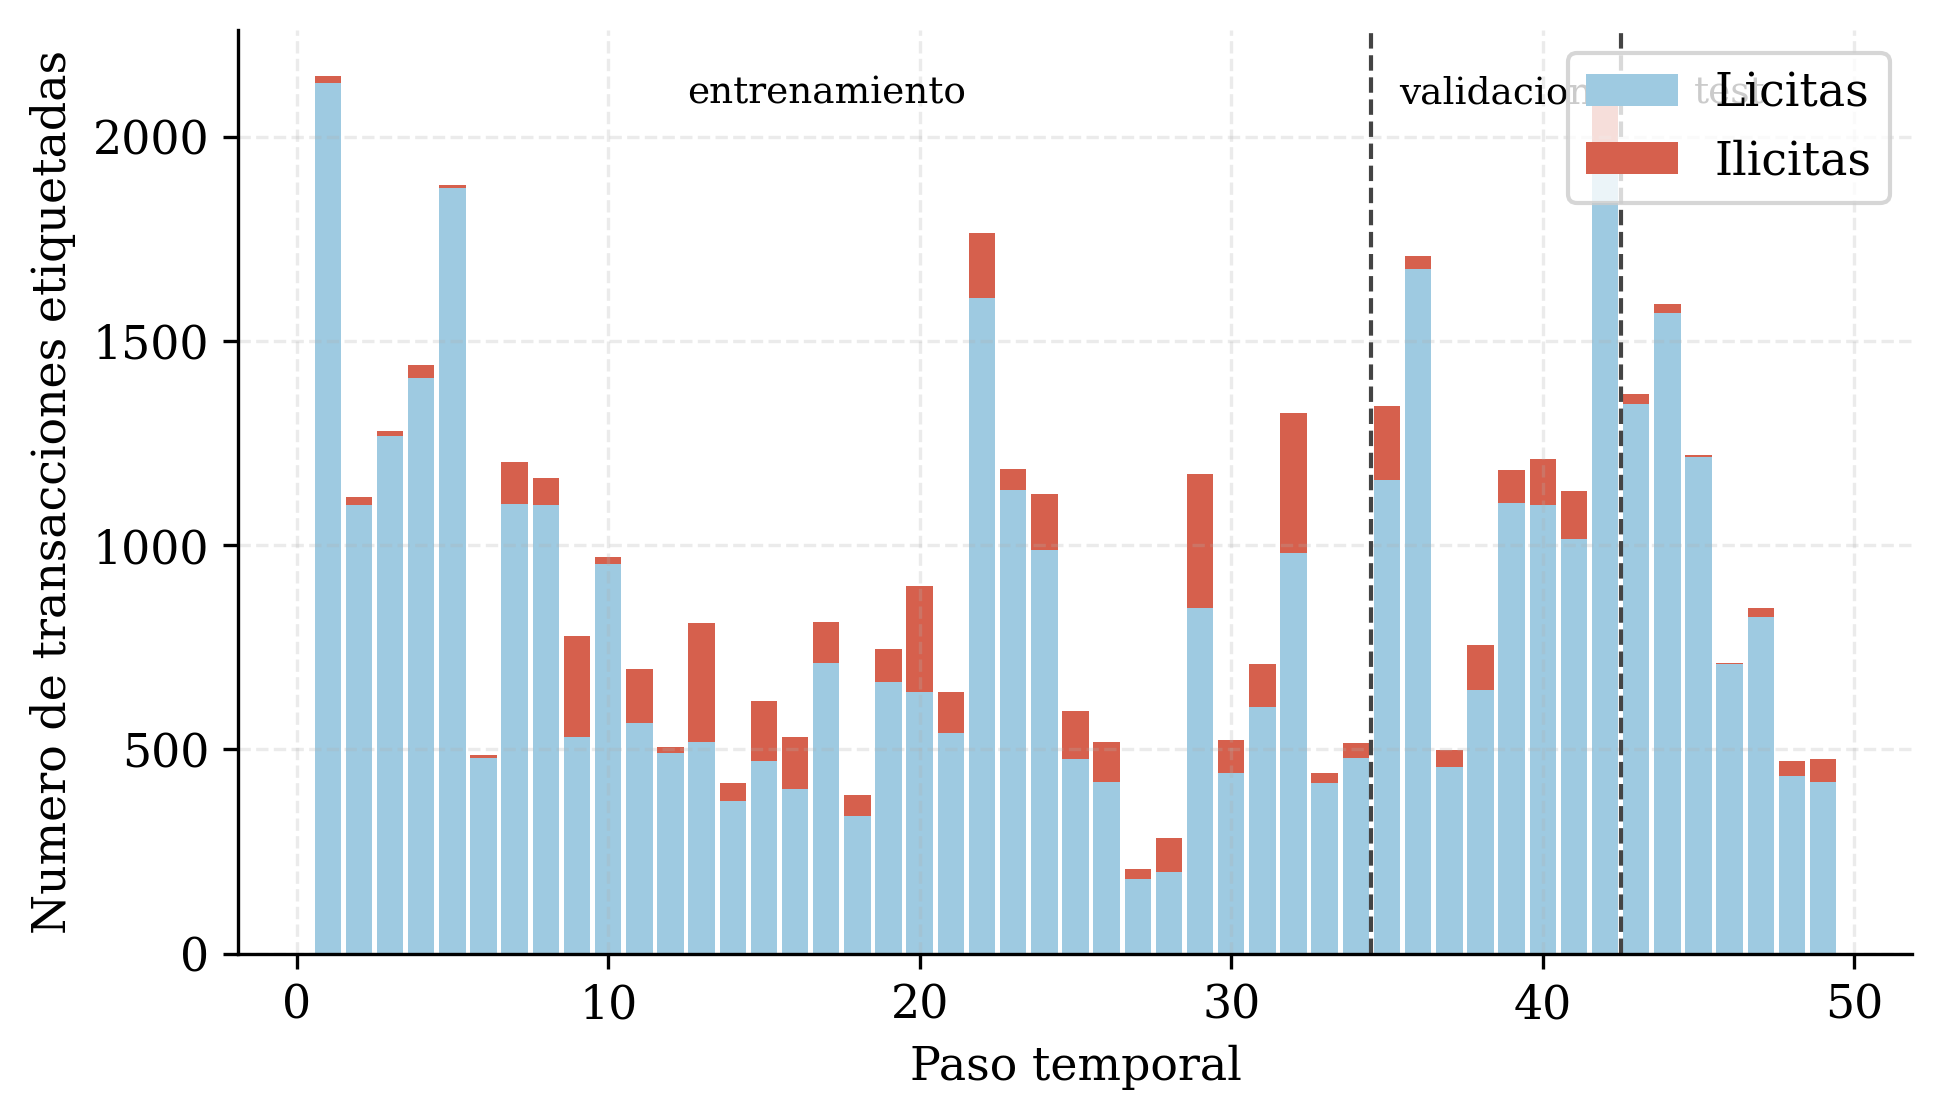
\includegraphics[width=0.85\textwidth]{chapter_4/images_ch4/eda_clases_timestep.png}
    \caption{Distribución de las transacciones etiquetadas del \textit{Elliptic Dataset} a lo largo de los 49 pasos temporales, con las particiones de entrenamiento, validación y test delimitadas. Tanto el volumen total como la proporción de actividad ilícita varían entre periodos, lo que anticipa el desplazamiento temporal que degrada la generalización.}
    \label{fig:eda-clases}
\end{figure}

La estructura temporal del conjunto tiene una implicación que se retoma en la Sección 4.4, la de que los patrones que caracterizan la actividad ilícita no son estacionarios. Un modelo que aprende a discriminar transacciones ilícitas en los primeros pasos temporales se enfrenta, en los últimos pasos, a una distribución que ha cambiado, lo que anticipa la dificultad de generalizar del periodo de entrenamiento al de test. Esta no estacionariedad es una propiedad del fenómeno del lavado, cuyas tipologías evolucionan para evadir la detección, y no un defecto del conjunto de datos. Reconocerla desde el análisis exploratorio permite interpretar correctamente los resultados de rendimiento que se presentan más adelante.

\subsection{Dispersión de la Topología}

Una segunda propiedad del grafo resulta determinante para el resto del estudio y merece un análisis detallado, la dispersión extrema de su topología. La mayoría de los nodos poseen muy pocas conexiones, hasta el punto de que el grado mediano es de dos y el nonagésimo percentil se sitúa en tres, con una media de dos coma tres aristas por nodo, tal como ilustra la Figura \ref{fig:eda-grados}. La escasez es aún más marcada en la clase ilícita, ya que el noventa y tres coma dos por ciento de las transacciones ilícitas presentan dos aristas o menos. Esta característica no es un defecto del preprocesamiento sino una propiedad intrínseca de las transacciones de Bitcoin etiquetadas, y condiciona de manera profunda todo lo que puede medirse sobre las explicaciones.

\begin{figure}[htbp]
    \centering
    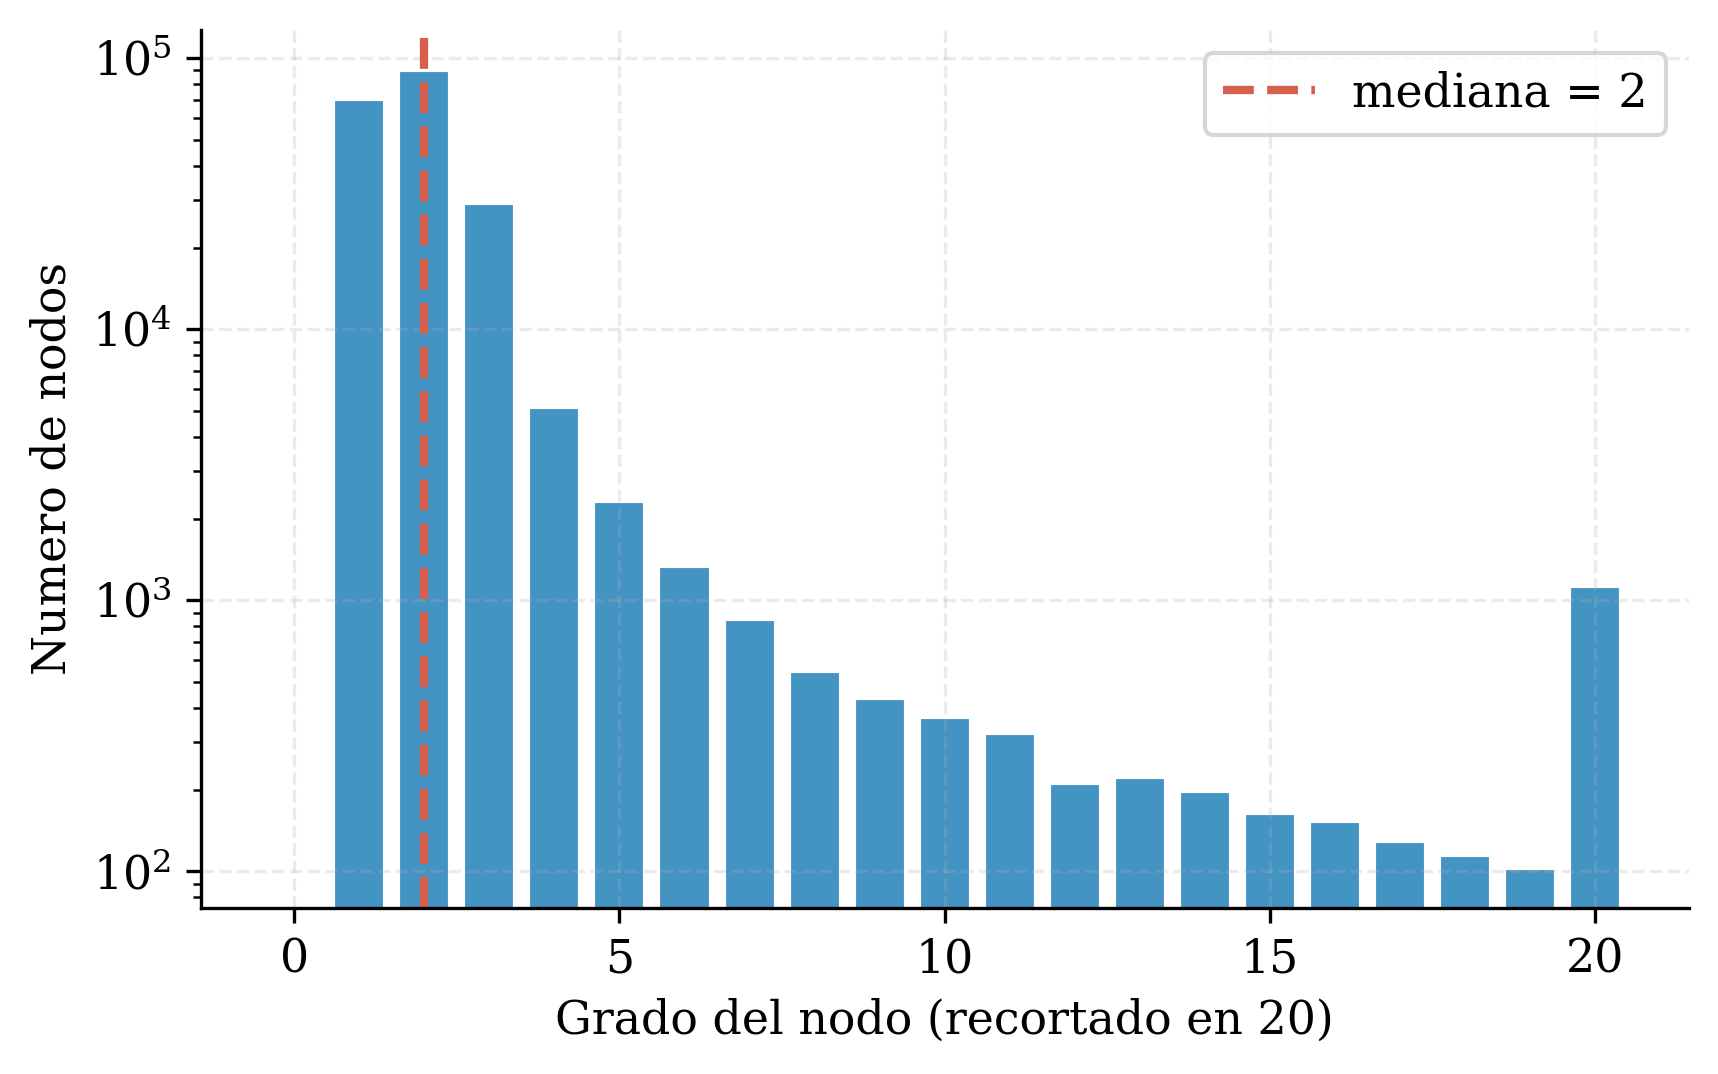
\includegraphics[width=0.75\textwidth]{chapter_4/images_ch4/eda_grados.png}
    \caption{Distribución del grado de los nodos del \textit{Elliptic Dataset} en escala logarítmica, recortada para su visualización. El grado mediano es de dos, lo que evidencia una topología extremadamente dispersa dominada por nodos con muy pocas conexiones.}
    \label{fig:eda-grados}
\end{figure}

La consecuencia directa de esta dispersión se aprecia al construir el subgrafo receptivo de un nodo, es decir el conjunto de nodos que influyen en su predicción a través del paso de mensajes. La mediana del tamaño de ese subgrafo es de apenas dos nodos, como muestra la Figura \ref{fig:dispersion}, de modo que un vecindario tan reducido deja muy poco margen para que una explicación estructural sea informativa o para que su plausibilidad sea medible. Esta limitación es la razón de fondo por la que el eje sintético del Capítulo 5 resulta necesario, ya que sin estructura de subgrafo no existe un patrón que una explicación pueda recuperar ni contra el cual pueda contrastarse.

\begin{figure}[htbp]
    \centering
    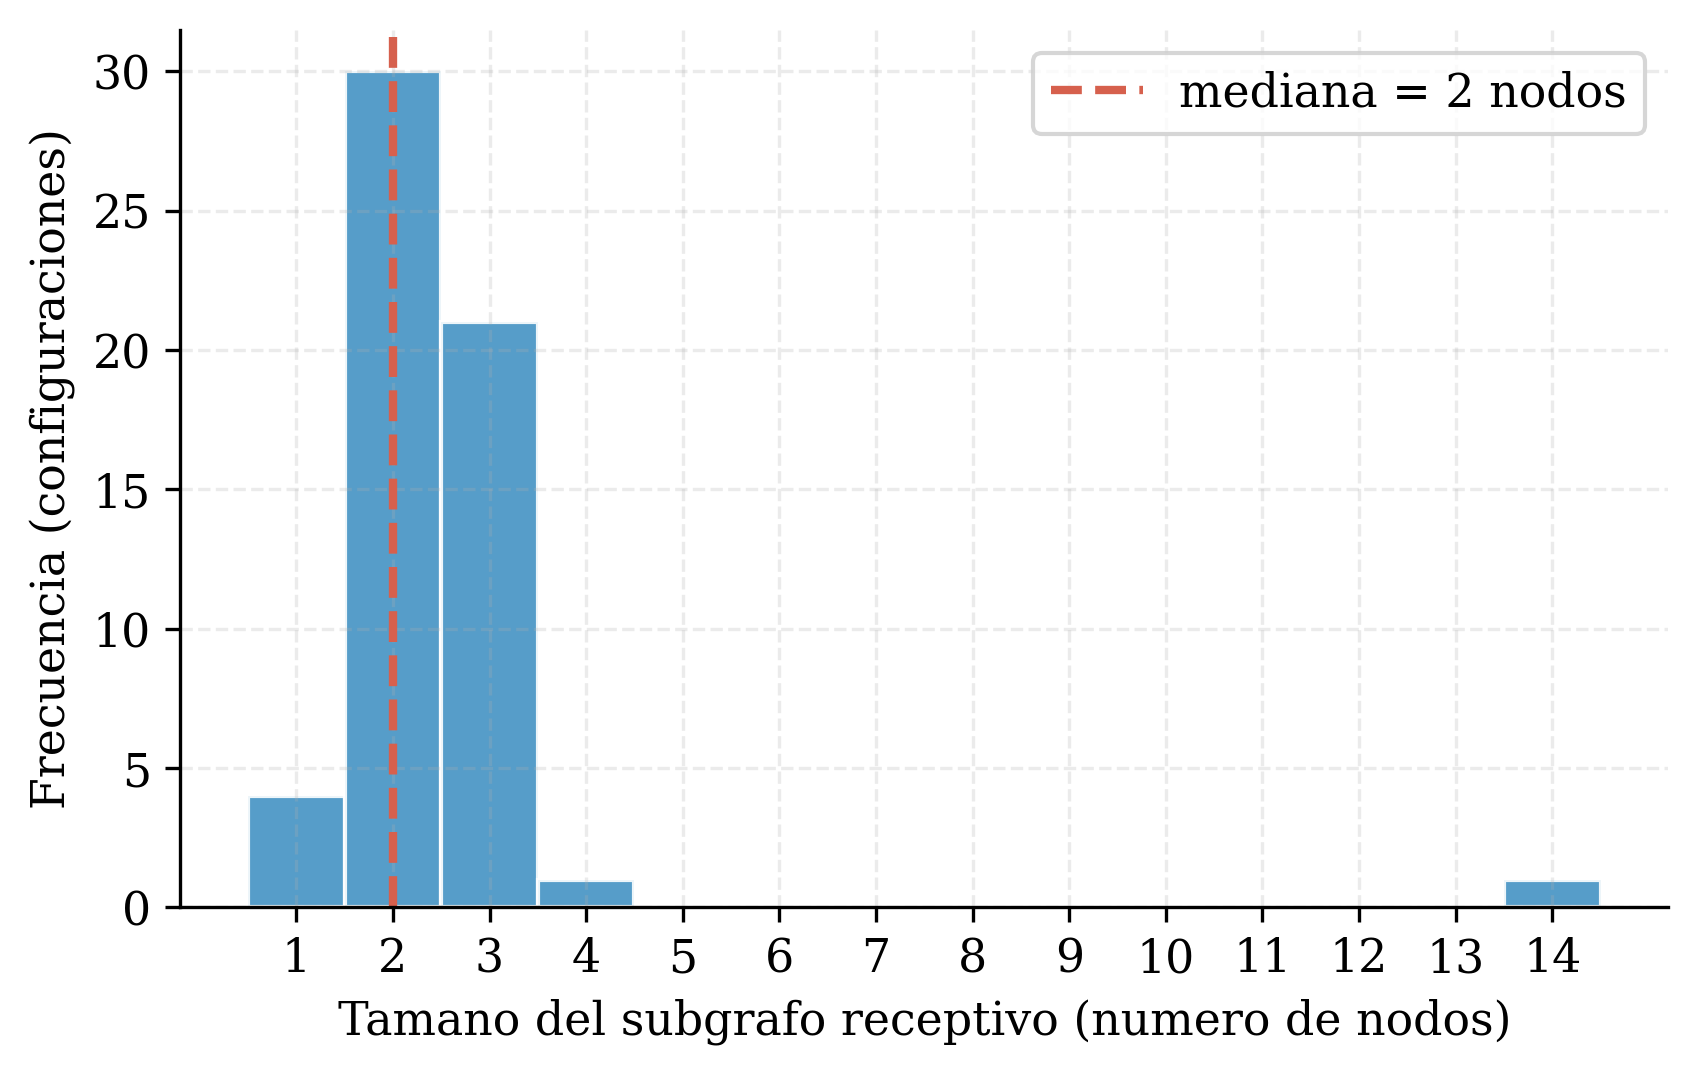
\includegraphics[width=0.8\textwidth]{chapter_4/images_ch4/dispersion_elliptic.png}
    \caption{Distribución del tamaño del subgrafo receptivo de los nodos ilícitos en el \textit{Elliptic Dataset}. La mediana se sitúa en dos nodos, lo que evidencia la dispersión extrema del grafo y explica por qué la plausibilidad estructural de las explicaciones no es medible en este dominio.}
    \label{fig:dispersion}
\end{figure}

La consecuencia inmediata de esta dispersión sobre la evaluación de estabilidad es que el índice de Jaccard entre aristas explicativas pierde buena parte de su capacidad de discriminar. Cuando el subgrafo receptivo contiene una o dos aristas, cualquier método que seleccione las aristas más relevantes recupera el mismo conjunto en cada ejecución, de modo que el índice de Jaccard se satura hacia valores altos, cercano a la unidad en los subgrafos más pequeños, y su media se mantiene comprimida alrededor de valores elevados con independencia de la arquitectura. La Tabla \ref{tab:jaccard} ilustra este efecto, ya que el Jaccard medio apenas varía entre arquitecturas, mientras que la correlación de Spearman de features se distribuye en un rango mucho más amplio y logra distinguir entre ellas. Por esta razón, y como se anticipó en el Capítulo 3, la correlación de Spearman entre los rankings de importancia de las features se adopta como la métrica de estabilidad informativa para el \textit{Elliptic Dataset}, dado que conserva sensibilidad incluso en vecindarios minúsculos, decisión metodológica que condiciona la lectura de todos los resultados de estabilidad que siguen.

\begin{table}[htbp]
\centering
\renewcommand{\arraystretch}{1.3}
\begin{tabular}{lcc}
\toprule
\textbf{Arquitectura} & \textbf{Jaccard medio} & \textbf{Spearman medio} \\
\midrule
GraphSAGE & 0,911 & 0,735 \\
GAT & 0,791 & 0,780 \\
GCN & 0,613 & 0,778 \\
TAGCN & 0,805 & 0,580 \\
\bottomrule
\end{tabular}
\caption{Comparación entre el índice de Jaccard de aristas y la correlación de Spearman de features (GNNExplainer) como métricas de estabilidad sobre el \textit{Elliptic Dataset}, con la métrica corregida. El Jaccard se satura hacia valores altos por la dispersión del grafo, mientras que la correlación de Spearman conserva capacidad de discriminación entre arquitecturas.}
\label{tab:jaccard}
\end{table}


\section{Pipeline Experimental y Espacio Factorial}

El diseño experimental se organiza como una matriz factorial que cruza cuatro dimensiones, a saber las cuatro arquitecturas GNN caracterizadas en el Capítulo 3, un conjunto de escenarios de desbalance, tres estrategias de balanceo y los tres métodos de explicabilidad. Las arquitecturas evaluadas son GCN, GraphSAGE, GAT y TAGCN, y ninguna recibe un tratamiento privilegiado dentro de la comparación. Las estrategias de balanceo comprenden el entrenamiento sin intervención, la ponderación de clases inversamente proporcional a su frecuencia y la Focal Loss \cite{Lin2017FocalDetection}, mientras que los explicadores son GNNExplainer, PGExplainer y GNNShap \cite{Ying2019Gnnexplainer:Networks, Luo2020ParameterizedNetwork, Akkas2024Gnnshap:Values}. El pipeline sigue cuatro fases, la preparación de los datos, el entrenamiento de los modelos con búsqueda de hiperparámetros, la generación de explicaciones y la medición de estabilidad mediante réplicas, tal como resume la Figura \ref{fig:metodologia}.

\begin{figure}[htbp]
    \centering
    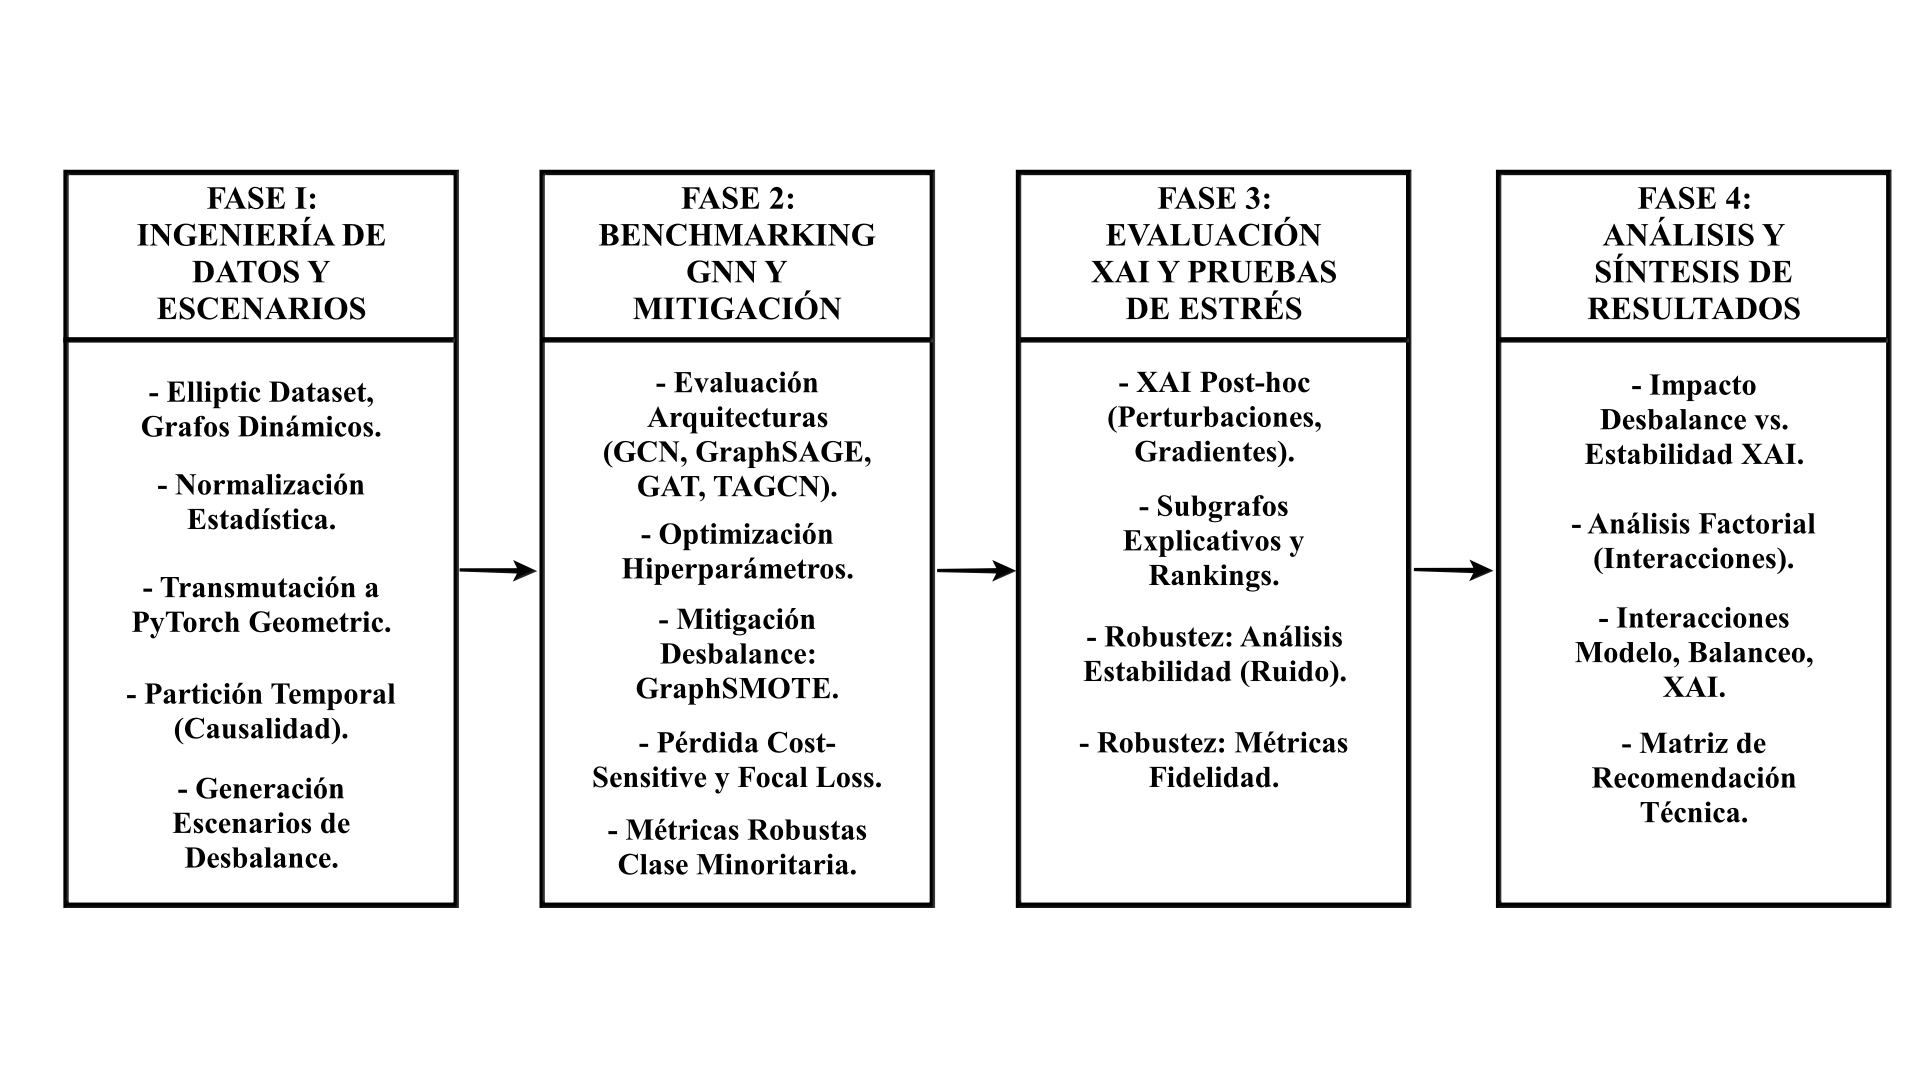
\includegraphics[width=0.9\textwidth]{chapter_4/images_ch4/metodologia.png}
    \caption{Metodología de cuatro fases del pipeline experimental, desde la preparación de los datos hasta la medición de estabilidad de las explicaciones mediante réplicas.}
    \label{fig:metodologia}
\end{figure}

El entrenamiento de cada modelo incorpora una búsqueda de hiperparámetros mediante optimización bayesiana, que ajusta la dimensión de las capas ocultas, el número de capas, la tasa de \textit{dropout} y la tasa de aprendizaje. La métrica que guía la búsqueda es el área bajo la curva de precisión y exhaustividad, más adecuada que la exactitud en presencia de desbalance extremo, y el criterio de parada temprana vigila el F1 de la clase ilícita para evitar detenerse por ruido. Este procedimiento busca que cada configuración alcance la mejor calidad posible antes de generar explicaciones, de manera que la estabilidad se mida sobre modelos que efectivamente aprendieron a discriminar y no sobre clasificadores triviales. La medición de estabilidad repite la explicación de cada nodo de interés cinco veces con semillas distintas y resume la variación resultante mediante la correlación de Spearman de los rankings de features.

\subsection{Compuerta de Calidad y Selección de Nodos a Explicar}

Un principio metodológico atraviesa todo el pipeline, el de que solo tiene sentido estudiar la estabilidad de las explicaciones de modelos que efectivamente aprendieron a discriminar. Para hacerlo operativo, cada configuración debe superar una compuerta de calidad antes de que se generen sus explicaciones, definida sobre la partición de validación mediante dos umbrales, un F1 de la clase ilícita no inferior a treinta centésimas y un coeficiente de correlación de Matthews no inferior a quince centésimas. Las configuraciones que no alcanzan estos umbrales se registran, pero se excluyen del subconjunto sobre el que se afirman las conclusiones, lo que evita que la estabilidad se mida sobre clasificadores triviales cuyas explicaciones carecen de significado. Esta compuerta es la razón por la que el ranking de estabilidad se presenta más adelante en dos corridas, una completa y otra restringida a las configuraciones que superan el filtro.

La selección de los nodos que se explican sigue el mismo principio de significado. Para cada configuración, se explican los nodos de la partición de validación que el modelo clasifica correctamente como ilícitos, es decir los verdaderos positivos, ya que solo en ellos existe una predicción positiva cuya explicación tiene interés analítico. Este criterio garantiza que la estabilidad medida corresponda a explicaciones de aciertos y no de errores, y que la comparación entre arquitecturas y explicadores se realice sobre un conjunto de nodos homogéneo en su condición de verdaderos positivos. El número de verdaderos positivos disponibles varía entre configuraciones, y ese número se registra junto con cada resultado para poder ponderar la confianza de las medias reportadas, tal como se detalla en la tabla completa del anexo.

\section{Escenarios de Desbalance}

Para estudiar el efecto del desbalance de clases sobre la estabilidad, el conjunto de entrenamiento se resamplea en cinco escenarios de proporción creciente entre transacciones ilícitas y lícitas. Los escenarios controlados corresponden a las razones 1:1, 1:10, 1:50 y 1:100, obtenidas mediante submuestreo de la clase mayoritaria, y se añade un escenario nativo que conserva la proporción del subconjunto etiquetado sin aplicar resampleo, cercana a 1:9. Esta gradación permite observar si la estabilidad de las explicaciones se degrada de forma monótona a medida que la clase ilícita se vuelve más escasa, o si presenta un comportamiento distinto. La inclusión del escenario nativo resulta relevante porque representa la condición realista del dato, sin manipulación artificial de la proporción, y ofrece un punto de comparación frente a los escenarios construidos.

\section{Rendimiento Predictivo y el Colapso de Validación a Test}

La evaluación del rendimiento bajo un desbalance tan extremo exige elegir la métrica con cuidado, puesto que el F1 calculado sobre un umbral fijo se vuelve degenerado cuando la clase positiva representa una fracción mínima del total. Por esa razón, la métrica primaria de este estudio es el área bajo la curva de precisión y exhaustividad, que resume la capacidad de ordenamiento del modelo sin depender de un umbral y que coincide con la magnitud pertinente en la práctica de la auditoría antilavado, donde el analista revisa un conjunto acotado de alertas de mayor puntuación en lugar de una decisión binaria sobre todo el universo de transacciones. Bajo esta métrica, los modelos alcanzan un rendimiento razonable sobre la partición de validación, con un valor de 0,52 en la mejor configuración hallada por la búsqueda de hiperparámetros y una media de 0,367 sobre los modelos que superan el filtro de calidad, lo que indica que el modelo aprende a situar las transacciones ilícitas por encima de las lícitas en el ordenamiento. Ese desempeño no se traslada a la partición de test, donde el área bajo la misma curva cae a un valor medio cercano a 0,013 sobre el conjunto de las sesenta configuraciones, y de 0,017 sobre las que superan el filtro de calidad, una caída que ninguna arquitectura evita y que el F1 en test, prácticamente nulo en las cuatro arquitecturas con valores de 0,0245 para GAT, 0,0133 para GCN, 0,0077 para GraphSAGE y 0,0015 para TAGCN, no hace sino reflejar de forma todavía más marcada, tal como recoge la Tabla \ref{tab:elliptic-perf}. Este fenómeno, que puede denominarse colapso de validación a test, constituye uno de los rasgos más importantes del dominio y condiciona la interpretación de todo el estudio.

\begin{table}[htbp]
\centering
\renewcommand{\arraystretch}{1.3}
\begin{tabular}{lccc}
\toprule
\textbf{Arquitectura} & \textbf{F1 (test)} & \textbf{MCC (test)} & \textbf{PR-AUC (test)} \\
\midrule
GraphSAGE & 0,008 & 0,003 & 0,017 \\
GAT & 0,025 & 0,017 & 0,014 \\
GCN & 0,013 & 0,008 & 0,010 \\
TAGCN & 0,001 & -0,006 & 0,011 \\
\bottomrule
\end{tabular}
\caption{Rendimiento predictivo medio en la particion de test por arquitectura sobre el \textit{Elliptic Dataset}. El colapso es generalizado, con valores de F1 y MCC muy bajos en las cuatro arquitecturas por efecto del desplazamiento temporal.}
\label{tab:elliptic-perf}
\end{table}


Para dimensionar el colapso con una perspectiva complementaria, se recalcularon sobre las particiones de validación y test dos familias de métricas de ordenamiento, el área bajo la curva ROC y la precisión en los primeros nodos de mayor puntuación, junto al área bajo la curva de precisión y exhaustividad, cuyos valores medios recoge la Tabla \ref{tab:elliptic-rocauc}. El contraste entre ellas es en sí mismo instructivo y refuerza la elección de la métrica primaria. Sobre validación, los modelos que superan el filtro de calidad alcanzan un ROC-AUC medio de 0,884 que sugeriría un clasificador casi excelente, pero el mismo conjunto arroja un área de precisión y exhaustividad de 0,367 y una precisión en los primeros cincuenta nodos de 0,657, cifras que revelan una tarea mucho más difícil de lo que el ROC-AUC insinúa. Sobre test la disociación se vuelve extrema, ya que el ROC-AUC se mantiene en 0,653, un valor que por sí solo parecería indicar un modelo apenas mediocre, mientras que el área de precisión y exhaustividad se desploma a 0,017 y la precisión en los primeros cincuenta nodos a 0,020, apenas por encima de la tasa base de transacciones ilícitas en el test. Esta discrepancia ilustra por qué el ROC-AUC resulta engañoso bajo desbalance extremo, puesto que su eje de tasa de falsos positivos queda dominado por la enorme clase mayoritaria y permanece bajo aunque el modelo no distinga la clase rara, lo que justifica adoptar el área de precisión y exhaustividad y la precisión en los primeros nodos como métricas primarias, que son ademas las que gobiernan el trabajo real de triaje en una auditoría antilavado.

\begin{table}[htbp]
\centering
\renewcommand{\arraystretch}{1.3}
\begin{tabular}{lcc}
\toprule
\textbf{Métrica de ordenamiento} & \textbf{Validación} & \textbf{Test} \\
\midrule
ROC-AUC & 0,884 & 0,653 \\
PR-AUC & 0,367 & 0,017 \\
Precisión en los primeros 50 & 0,657 & 0,020 \\
Precisión en los primeros 100 & 0,640 & 0,022 \\
\bottomrule
\end{tabular}
\caption{Métricas de ordenamiento medias sobre validación y test para los modelos que superan el filtro de calidad. El ROC-AUC se mantiene alto y engañoso bajo el desbalance extremo, mientras que el área de precisión y exhaustividad y la precisión en los primeros nodos revelan la dificultad real de la tarea y el colapso en test.}
\label{tab:elliptic-rocauc}
\end{table}

La causa del colapso no reside en un defecto del método sino en una propiedad estructural del dato, el desplazamiento temporal entre las particiones. El \textit{Elliptic Dataset} ordena las transacciones por pasos temporales, y los patrones que caracterizan la actividad ilícita en los primeros pasos difieren de los que aparecen en los últimos, de modo que un modelo ajustado sobre el periodo de validación encuentra en test una distribución distinta a la que aprendió \cite{Menezes2025SemanticDetectors}. Trabajos previos sobre el mismo conjunto de datos han documentado la fragilidad de los detectores basados en grafos ante este tipo de desplazamiento, lo que refuerza que se trata de una limitación del dato y no de la implementación \cite{Lawal2025AnDataset}. Reconocer esta limitación de forma explícita es preferible a ocultarla, ya que delimita con honestidad el alcance de las conclusiones. En consecuencia, y puesto que el objeto de la tesis es la estabilidad de las explicaciones y no el rendimiento predictivo en test, el estudio de estabilidad se realiza sobre los nodos de la partición de validación que el modelo clasifica correctamente como ilícitos.

Conviene precisar el sentido de esta decisión para evitar malentendidos. Estudiar la estabilidad sobre validación no busca disimular el colapso, sino situar el análisis allí donde el modelo efectivamente discrimina y donde, por tanto, la pregunta por la estabilidad de una explicación tiene sentido. Un modelo que no detecta ninguna transacción ilícita en test no genera predicciones positivas cuya explicación pueda evaluarse, de manera que forzar la medición sobre test produciría explicaciones de predicciones erróneas y carentes de interés analítico. La estabilidad reportada en las secciones siguientes se refiere, por tanto, a las explicaciones de verdaderos positivos sobre validación, un encuadre que se declara de forma transparente y que constituye una respuesta metodológica honesta ante una limitación estructural del dato.

\section{De un Artefacto de Cómputo a un Artefacto de Medida: dos Correcciones Metodológicas}

La forma en que se generan las explicaciones tiene un efecto inesperado y de gran alcance sobre los resultados de estabilidad. En una primera versión del pipeline, cada explicación se calculaba sobre el grafo completo de 203.769 nodos, lo que imponía una carga de memoria considerable a los explicadores basados en máscaras. En el caso de GAT, cuyo mecanismo de atención multiplica el consumo de memoria por el número de cabezas, esa carga provocaba fallos por agotamiento de memoria de la unidad de procesamiento gráfico, con picos cercanos a 7,5 GiB. El problema más serio no era el fallo en sí, sino que trece de esas configuraciones de GAT fallaban de forma silenciosa y sus filas quedaban vacías, de modo que el promedio de estabilidad de GAT terminaba calculándose solo sobre las siete u ocho configuraciones que sí completaban la ejecución.

Este comportamiento generaba un artefacto grave que conviene exponer con detalle. El ranking de estabilidad de la versión anterior situaba a GAT como la arquitectura más estable, con un valor cercano a 0,534, por encima de GraphSAGE, que aparecía como la peor con 0,345, pero esa comparación no era legítima porque GAT se medía sobre un subconjunto favorable de sus configuraciones mientras GraphSAGE se medía sobre todas. La primera corrección consiste en calcular cada explicación sobre el subgrafo receptivo del nodo de interés, es decir el conjunto de nodos que realmente influyen en su predicción según el número de capas de la arquitectura, en lugar de sobre el grafo completo. Para TAGCN, cuyo campo receptivo se amplía por el orden del filtro polinomial, se emplea un radio de dos saltos. Esta restricción reduce el consumo de memoria de 7,5 GiB a 0,02 GiB y elimina por completo los fallos, de manera que las cuatro arquitecturas pasan a medirse sobre el mismo soporte y en condiciones equitativas.

La medición sobre el subgrafo receptivo, con todo, seguía descansando sobre una implementación defectuosa de la propia métrica de estabilidad, cuya reparación constituye la segunda corrección. La correlación de Spearman entre rankings de features se calculaba descartando toda feature cuyo índice superara el parámetro de truncamiento, fijado en veinte para el Elliptic Dataset, lo que equivalía a comparar rankings mutilados y deprimía de forma sistemática la concordancia medida. La reparación conserva la longitud completa de cada ranking y asigna un rango común a las features situadas fuera del conjunto principal, en lugar de eliminarlas. Un rasgo decisivo para la interpretación es que el efecto de esta reparación no es uniforme entre arquitecturas, porque el truncamiento penalizaba con mayor severidad a aquellas cuya importancia se reparte sobre un número mayor de features.

Al recomputar la estabilidad con la métrica corregida sobre el subconjunto de veintitrés configuraciones que superan el filtro de calidad, el mismo que la tesis utiliza para sus conclusiones, la ventaja de GraphSAGE desaparece y el orden vuelve a modificarse. GAT alcanza una correlación media de 0,779 sobre siete configuraciones, por encima de GraphSAGE con 0,743 sobre once, mientras que GCN queda en 0,833 sobre una única configuración y TAGCN en 0,641 sobre cuatro, tal como recoge la Tabla \ref{tab:ranking} y visualiza la Figura \ref{fig:ranking}. La reparación elevó a GAT en 0,244 puntos y a TAGCN en 0,278, frente a un ascenso de apenas 0,103 en GraphSAGE, lo que identifica al truncamiento de la métrica como la causa de la aparente superioridad de GraphSAGE que reportaba la versión anterior. La comparación restringida a las siete configuraciones en que GAT y GraphSAGE superan ambos el filtro, un contraste libre de sesgo de selección, sostiene el mismo sentido, puesto que GAT promedia 0,779 frente a 0,739 de GraphSAGE, cuando con la métrica defectuosa el orden era el inverso, de 0,535 frente a 0,627. El mismo orden se observa sobre la corrida completa de las sesenta configuraciones, donde GAT y GCN encabezan con 0,780 y 0,778, por delante de GraphSAGE con 0,735 y de TAGCN con 0,580, lo que confirma que la conclusión no depende del filtro de calidad.

\begin{figure}[htbp]
    \centering
    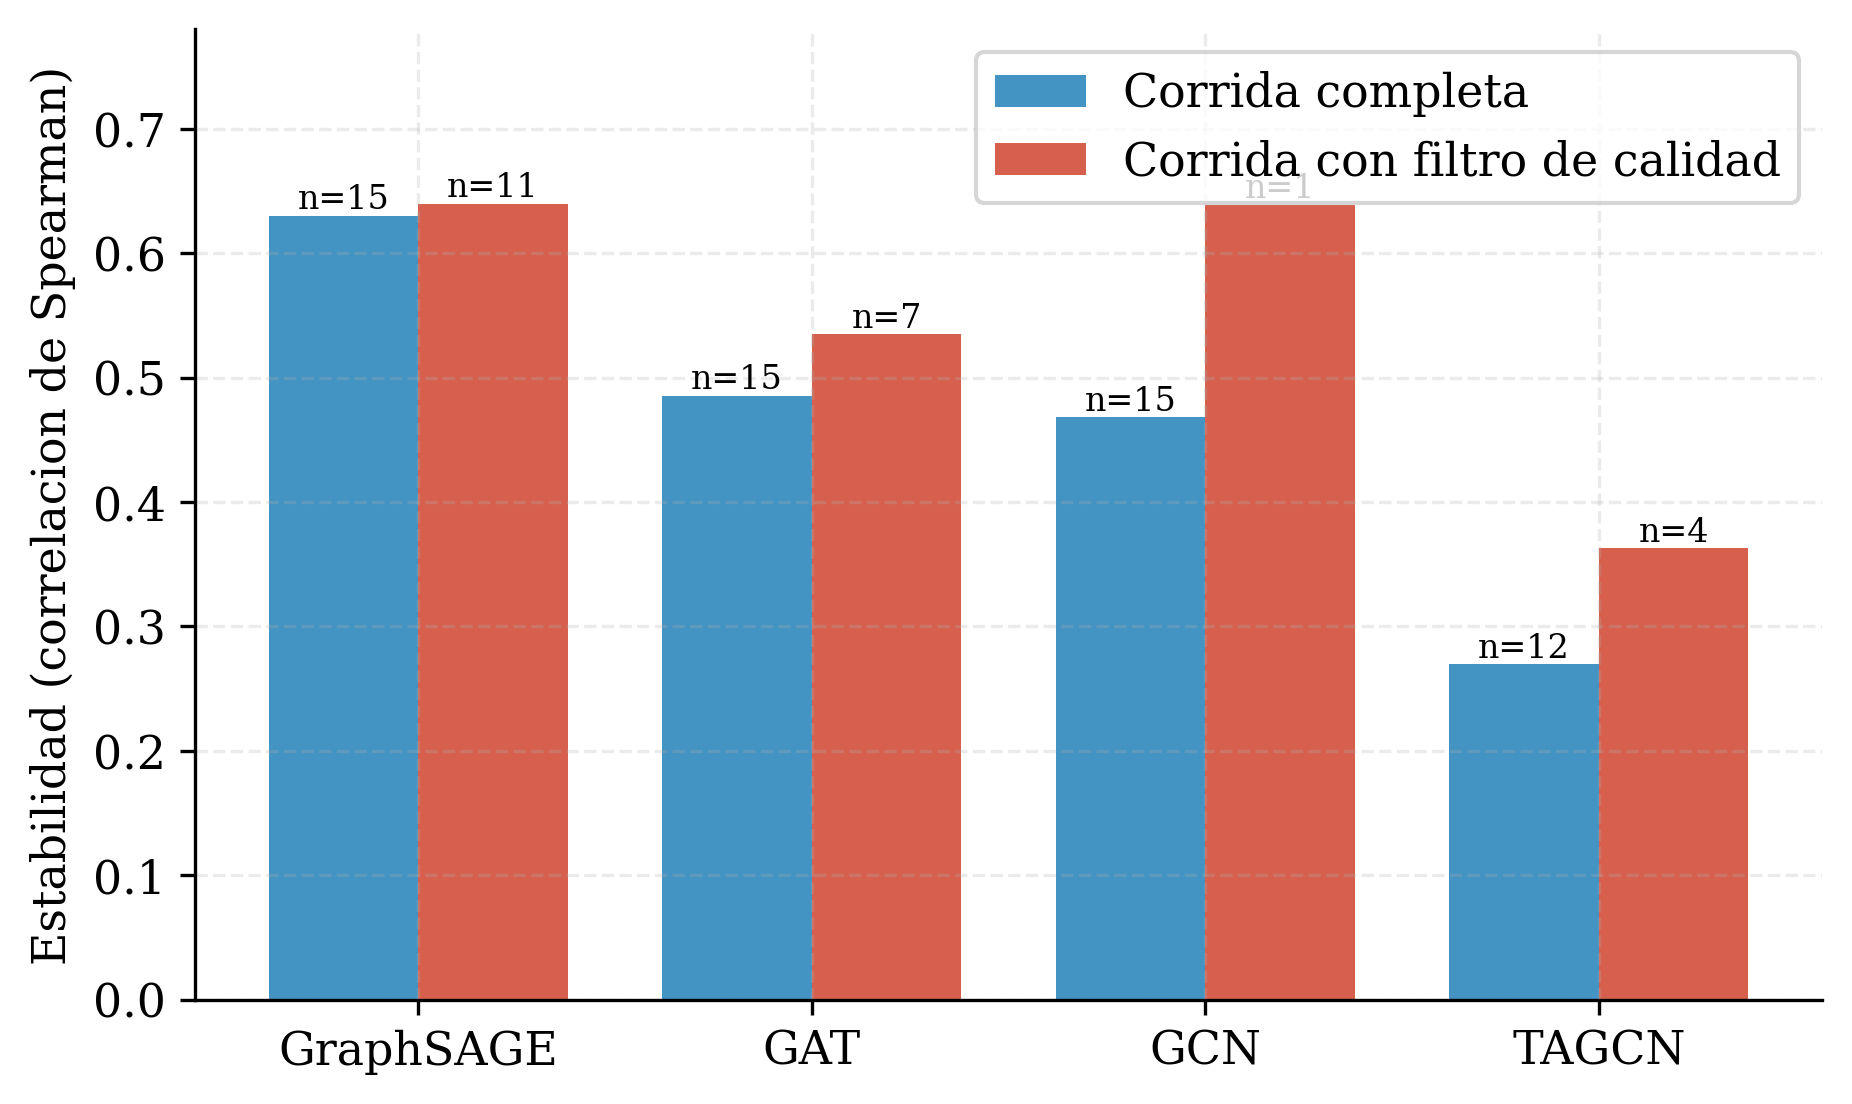
\includegraphics[width=0.85\textwidth]{chapter_4/images_ch4/ranking_khop.png}
    \caption{Estabilidad de las explicaciones por arquitectura sobre el subgrafo receptivo y con la métrica de Spearman corregida, promediada sobre las tres semillas de modelo, con barras de error que representan la desviación típica entre semillas. La prueba de rangos con signo separa un grupo alto formado por GAT y GCN de un grupo bajo formado por GraphSAGE y TAGCN, con diferencias significativas entre grupos y no dentro del grupo bajo. La mayor dispersión de TAGCN advierte contra fijar su valor central con demasiada precisión.}
    \label{fig:ranking}
\end{figure}

La lectura que esta tesis afirma como robusta debe revisarse a la luz de la métrica corregida, y el resultado es más prudente que el de la versión anterior. Ninguna arquitectura domina la estabilidad de forma transversal, y la superioridad de GraphSAGE sobre GAT que la versión previa reportaba no sobrevive a la reparación de la métrica. Sobre el subconjunto con calidad garantizada, GAT y GraphSAGE resultan prácticamente indistinguibles, con una diferencia de cuatro centésimas sostenida sobre siete y once configuraciones, mientras que GCN se apoya en una sola configuración y TAGCN en cuatro, un soporte insuficiente para fijar su posición relativa. La afirmación que sí se sostiene, y que gana fuerza al contrastarse con el eje sintético del Capítulo 5, es que el orden de estabilidad corregido en Elliptic concuerda con el del grafo denso, en el que GCN y GAT encabezan la estabilidad de GNNExplainer, de modo que la resiliencia de estas arquitecturas se manifiesta con relativa independencia de la densidad del grafo.

La prudencia de esta lectura se apoya en un contraste estadístico explícito. La diferencia de estabilidad entre GAT y GraphSAGE sobre las siete configuraciones en que ambos superan el filtro, de apenas cuatro centésimas, no alcanza significación estadística, ni con la prueba de rangos con signo de Wilcoxon, que arroja un valor p de 0,375, ni con la prueba t pareada, con un valor p de 0,380. Los intervalos de confianza al noventa y cinco por ciento de sus medias se solapan de forma amplia, de 0,705 a 0,853 para GAT y de 0,720 a 0,766 para GraphSAGE. Conviene subrayar el origen de esta indeterminación, que no reside en que las arquitecturas sean equivalentes sino en que una sola inicialización sobre un soporte reducido carece de potencia para separarlas. La sección siguiente levanta precisamente esa limitación mediante una replicación con tres semillas de modelo, y con ella la comparación entre GAT y GraphSAGE sí alcanza significación, de manera que la cautela expresada aquí debe leerse como una restricción del diseño de una sola semilla y no como una conclusión sobre las arquitecturas.

La sucesión de las dos correcciones encierra un valor metodológico que trasciende el resultado puntual. Un primer artefacto, de naturaleza computacional, favorecía a GAT mediante un cálculo sobre el grafo completo que fallaba de forma silenciosa y dejaba fuera sus configuraciones más costosas; un segundo artefacto, de naturaleza métrica, favorecía a GraphSAGE mediante un truncamiento que mutilaba los rankings de features y penalizaba con más fuerza a las arquitecturas de importancia más repartida. Cada uno de ellos, por separado, bastaba para producir una conclusión comparativa llamativa y falsa, y solo la corrección de ambos permite una lectura estable de los datos. Este doble episodio ilustra de forma concreta la advertencia de Kosan y colaboradores sobre la sensibilidad de las conclusiones al protocolo de evaluación, y refuerza la necesidad de auditar las condiciones de cómputo y de medida con el mismo rigor que se aplica a los métodos \cite{Kosan2023GNNX-BENCH:Benchmarking}.

\section{Replicación con Múltiples Semillas y Estructura en Dos Grupos}

Las conclusiones expuestas hasta aquí descansaban sobre una única inicialización del entrenamiento, lo que impedía separar una diferencia real entre arquitecturas del ruido propio de un ajuste concreto. Para levantar esa limitación, la matriz completa de sesenta configuraciones se reentrenó con tres semillas de modelo independientes, cada una ejecutando el procedimiento entero, incluida su propia búsqueda de hiperparámetros, hasta totalizar ciento ochenta modelos sobre los que se recalculó la estabilidad de GNNExplainer. Mantener la búsqueda dentro de la replicación, en lugar de reutilizar los hiperparámetros de la primera semilla, responde al propósito de medir la variabilidad del procedimiento completo y no solo la de la inicialización de los pesos, que es la pregunta pertinente cuando lo que se desea establecer es si una conclusión depende de una corrida particular.

La replicación arroja en primer término un resultado sobre reproducibilidad que conviene declarar con precisión. Reentrenar con la misma semilla no devuelve modelos idénticos, ya que las operaciones de dispersión que implementan el paso de mensajes sobre la unidad de procesamiento gráfico emplean sumas atómicas cuyo orden no es determinista, de modo que la reproducibilidad exacta a nivel de pesos no es alcanzable sin renunciar al rendimiento. Lo que sí se reproduce, y es lo que importa para una afirmación científica, son las conclusiones, puesto que el reentrenamiento independiente de la matriz devolvió el mismo filtro de calidad, con veinticinco configuraciones superándolo frente a las veintitrés originales, y el mismo orden de estabilidad entre arquitecturas. La distinción entre reproducibilidad de los pesos y reproducibilidad de las conclusiones es pertinente para cualquier trabajo que entrene redes sobre grafos en aceleradores gráficos, y omitirla induce expectativas que el cómputo no puede satisfacer.

Los valores medios por arquitectura y semilla, que recoge la Tabla \ref{tab:seeds}, sostienen el orden reportado en la sección anterior y a la vez precisan su lectura. GAT encabeza con una media de 0,782 y una desviación típica de 0,013, seguido de GCN con 0,757, GraphSAGE con 0,735 y TAGCN con 0,672. Las dos primeras posiciones se permutan entre semillas, ya que GCN encabeza en una de ellas y GAT en las otras dos, lo que confirma de forma empírica la cautela con la que la sección anterior se negaba a nombrar una única arquitectura ganadora. TAGCN, por su parte, resulta ser la arquitectura con mayor dispersión entre semillas con diferencia, con una desviación típica de 0,077 frente a valores comprendidos entre 0,013 y 0,025 en las restantes, de manera que el valor de 0,580 que arrojaba la semilla única correspondía al extremo bajo de su rango y no a su comportamiento típico.

\begin{table}[htbp]
    \centering
    \renewcommand{\arraystretch}{1.3}
    \begin{tabular}{lccccc}
    \toprule
    \textbf{Arquitectura} & \textbf{Semilla 42} & \textbf{Semilla 43} & \textbf{Semilla 44} & \textbf{Media} & \textbf{Desv. típica} \\
    \midrule
    GAT       & 0,766 & 0,789 & 0,790 & 0,782 & 0,013 \\
    GCN       & 0,783 & 0,733 & 0,757 & 0,757 & 0,025 \\
    GraphSAGE & 0,756 & 0,713 & 0,738 & 0,735 & 0,022 \\
    TAGCN     & 0,586 & 0,693 & 0,736 & 0,672 & 0,077 \\
    \bottomrule
    \end{tabular}
    \caption{Estabilidad media de las explicaciones de GNNExplainer por arquitectura y semilla de modelo sobre el Elliptic Dataset, con la métrica de Spearman corregida. Las dos primeras posiciones se permutan entre semillas, mientras que TAGCN exhibe una dispersión tres veces mayor que la de cualquier otra arquitectura.}
    \label{tab:seeds}
\end{table}

La potencia inferencial que aporta la replicación permite sustituir un ordenamiento de cuatro posiciones por una estructura más simple y mejor sostenida. Sobre las celdas comunes de escenario, balanceo y semilla, la prueba de rangos con signo de Wilcoxon separa con claridad dos grupos. GAT y GCN resultan indistinguibles entre sí, con un valor p de 0,165, y ambos superan de forma significativa a GraphSAGE, con valores p de 0,0033 y 0,047 respectivamente, y a TAGCN, con valores p inferiores a 0,0001 y de 0,0067. En el extremo opuesto, GraphSAGE y TAGCN tampoco se distinguen entre sí, con un valor p de 0,096. La lectura correcta de la estabilidad por arquitectura en Elliptic no es, por tanto, un ranking de cuatro puestos sino una partición en un grupo alto formado por GAT y GCN y un grupo bajo formado por GraphSAGE y TAGCN, con diferencias significativas entre grupos y no dentro de ellos.

La partición resiste además el contraste con una familia de pruebas distinta de la empleada hasta aquí, lo que descarta que sea un artefacto del diseño pareado. La prueba de Kruskal-Wallis sobre las cuatro arquitecturas rechaza la hipótesis de igualdad con un estadístico de 23,79 y un valor p de 2,8 por diez elevado a menos cinco, con un tamaño de efecto epsilon cuadrado de 0,125 que corresponde a una magnitud media. Al aplicar la misma prueba dentro de cada grupo, en cambio, la igualdad no se rechaza, ni entre GAT y GCN, con un valor p de 0,192, ni entre GraphSAGE y TAGCN, con un valor p de 0,080. La comparación no pareada entre el conjunto de las dos arquitecturas del grupo alto y el de las dos del grupo bajo, mediante la prueba de Mann-Whitney, arroja un valor p de 1,4 por diez elevado a menos seis. El patrón es por tanto consistente, ya que la variabilidad entre arquitecturas se concentra entre grupos y no dentro de ellos.

Los intervalos de confianza bootstrap que recoge la Tabla \ref{tab:ic} ofrecen la misma lectura en forma de estimación por intervalo. El intervalo de GAT, de 0,758 a 0,805, y el de GCN, de 0,724 a 0,787, se solapan de forma amplia, al igual que el de GraphSAGE, de 0,710 a 0,756, con el de TAGCN, de 0,632 a 0,717. Entre grupos, en cambio, los intervalos de GAT y de GraphSAGE apenas se tocan, y el de TAGCN es el más ancho de los cuatro, con una amplitud de 0,085 que casi duplica la de GAT y que refleja la mayor dispersión entre semillas ya señalada.

\begin{table}[htbp]
    \centering
    \renewcommand{\arraystretch}{1.3}
    \begin{tabular}{lcccc}
    \toprule
    \textbf{Arquitectura} & \textbf{n} & \textbf{Media} & \textbf{IC95 inferior} & \textbf{IC95 superior} \\
    \midrule
    GAT       & 45 & 0,782 & 0,758 & 0,805 \\
    GCN       & 44 & 0,758 & 0,724 & 0,787 \\
    GraphSAGE & 42 & 0,735 & 0,710 & 0,756 \\
    TAGCN     & 40 & 0,676 & 0,632 & 0,717 \\
    \bottomrule
    \end{tabular}
    \caption{Estabilidad media por arquitectura sobre el Elliptic Dataset e intervalos de confianza al noventa y cinco por ciento obtenidos por remuestreo bootstrap con diez mil réplicas, agregando las tres semillas de modelo. Los intervalos se solapan dentro de cada grupo y apenas se tocan entre grupos, en coherencia con las pruebas de hipótesis. La mayor amplitud del intervalo de TAGCN refleja su elevada dispersión entre semillas.}
    \label{tab:ic}
\end{table}

Esta estructura corrige y a la vez fortalece lo afirmado con una sola semilla. Fortalece, porque la comparación entre GAT y GraphSAGE, que con una semilla no alcanzaba significación y obligaba a una formulación cautelosa, pasa a ser significativa con un valor p de 0,0033, de modo que ahora puede sostenerse que el grupo alto supera al resto y no solamente que lo encabeza. Corrige, porque la afirmación de que TAGCN quedaba netamente rezagada no sobrevive a la replicación, dado que su distancia respecto de GraphSAGE no alcanza significación estadística. Lo que sí se mantiene, y es lo que la hipótesis de trabajo comprometía, es que TAGCN no resulta la arquitectura más estable pese a su alcance multisalto, ya que aparece de forma consistente en el grupo bajo en las tres semillas.

Un último aspecto refuerza la solidez de esta partición. El eje sintético del Capítulo 5, medido de forma independiente sobre un régimen de densidad opuesto y con su propia replicación, exhibe exactamente la misma estructura, con GCN en 0,965 y GAT en 0,960 muy por encima de GraphSAGE en 0,889 y TAGCN en 0,886, valores que separan dos grupos con la misma composición y con diferencias internas mínimas. Que dos regímenes tan distintos, medidos con datos y con pipelines separados, converjan en la misma partición constituye un respaldo considerablemente más fuerte que la coincidencia de un orden entre cuatro posiciones, y refuerza la lectura conjunta que desarrolla el Capítulo 6.

\begin{table}[htbp]
    \centering
    \renewcommand{\arraystretch}{1.3}
    \begin{tabular}{lccc}
    \toprule
    \textbf{Arquitectura} & \textbf{Corrida completa (n)} & \textbf{Corrida con filtro (n)} & \textbf{Tres semillas} \\
    \midrule
    GAT       & 0,780 (15) & 0,779 (7)  & 0,782 $\pm$ 0,013 \\
    GCN       & 0,778 (15) & 0,833 (1)  & 0,757 $\pm$ 0,025 \\
    GraphSAGE & 0,735 (15) & 0,743 (11) & 0,735 $\pm$ 0,022 \\
    TAGCN     & 0,580 (12) & 0,641 (4)  & 0,672 $\pm$ 0,077 \\
    \bottomrule
    \end{tabular}
    \caption{Estabilidad de las explicaciones (correlación de Spearman) por arquitectura sobre el subgrafo receptivo y con la métrica corregida. Las dos primeras columnas corresponden a la semilla original, con el número de configuraciones de soporte entre paréntesis, y la tercera a la media y la desviación típica sobre las tres semillas de la replicación descrita en la sección siguiente. Con la métrica reparada, GAT y GCN encabezan las tres columnas y la anterior ventaja de GraphSAGE no se sostiene. El soporte de la corrida con filtro es desigual, ya que GCN se apoya en una única configuración y TAGCN en cuatro, de modo que esa columna se reporta como control de consistencia y no como estimación. La replicación resuelve esa limitación y sitúa a TAGCN en 0,672, bastante por encima del valor que arrojaba la semilla única, además de revelar que es la arquitectura con mayor dispersión entre semillas.}
    \label{tab:ranking}
\end{table}

El comportamiento de la estabilidad a lo largo de los escenarios de desbalance confirma que este factor no gobierna la reproducibilidad de las explicaciones. Con la métrica corregida, el perfil es esencialmente plano, con valores medios que van de 0,709 en el escenario nativo a 0,741 en el escenario 1:100, pasando por 0,723 en 1:1, 0,726 en 1:10 y 0,727 en 1:50, como ilustra la Figura \ref{fig:escenario} y detalla por arquitectura la Tabla \ref{tab:elliptic-stab-scen}. La amplitud total entre escenarios, de apenas tres centésimas, indica que el nivel de desbalance no produce un deterioro monótono ni un punto de quiebre localizado. En consecuencia desaparece tanto el supuesto pico de inestabilidad en el escenario 1:50 como cualquier paradoja atribuida al escenario nativo, ya que ningún punto destaca sobre los demás. Esta planitud resulta coherente con el hallazgo, desarrollado en el eje sintético, de que el desbalance es un factor secundario frente al explicador y la arquitectura.

\begin{figure}[htbp]
    \centering
    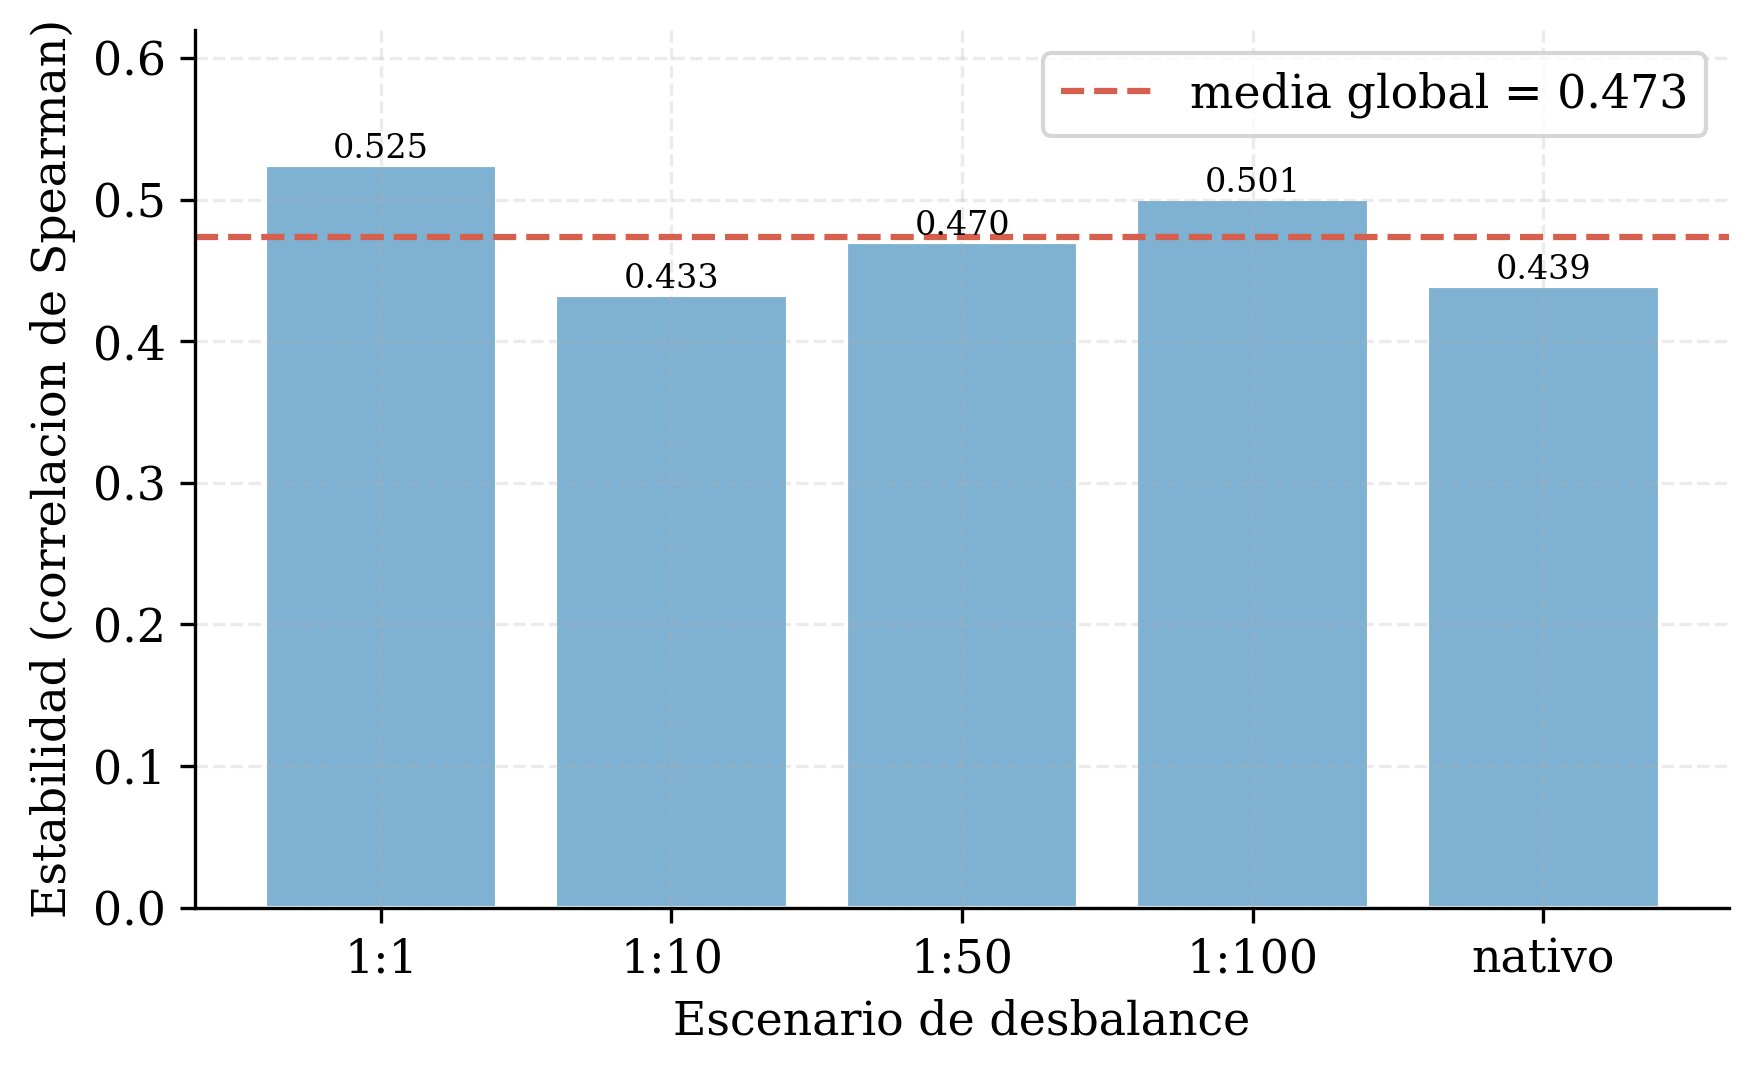
\includegraphics[width=0.8\textwidth]{chapter_4/images_ch4/estabilidad_escenario.png}
    \caption{Estabilidad de las explicaciones por escenario de desbalance sobre el subgrafo receptivo. El perfil es esencialmente plano, sin un pico de inestabilidad en el escenario 1:50 y con el valor más bajo en el escenario nativo, lo que invalida la interpretación previa de un deterioro localizado.}
    \label{fig:escenario}
\end{figure}

\begin{table}[htbp]
\centering
\renewcommand{\arraystretch}{1.3}
\begin{tabular}{lccccc}
\toprule
\textbf{Arquitectura} & 1:1 & 1:10 & 1:50 & 1:100 & nativo \\
\midrule
GraphSAGE & 0,715 & 0,748 & 0,761 & 0,697 & 0,751 \\
GAT & 0,750 & 0,811 & 0,798 & 0,765 & 0,785 \\
GCN & 0,697 & 0,760 & 0,787 & 0,757 & 0,793 \\
TAGCN & 0,622 & 0,626 & 0,703 & 0,752 & 0,704 \\
\midrule
\textbf{Media} & 0,696 & 0,736 & 0,765 & 0,745 & 0,760 \\
\bottomrule
\end{tabular}
\caption{Estabilidad de las explicaciones (correlación de Spearman de GNNExplainer) por arquitectura y escenario de desbalance sobre el subgrafo receptivo, promediada sobre las tres semillas de modelo. GCN y GAT encabezan la estabilidad de forma transversal a los escenarios, y la fila de medias muestra que el nivel de desbalance no ordena los resultados.}
\label{tab:elliptic-stab-scen}
\end{table}


La corrección obliga además a retractar el supuesto compromiso entre exactitud y estabilidad que la versión anterior reportaba con una correlación cercana a -0,20. Al haberse recomputado la estabilidad con una métrica corregida, aquella correlación deja de ser válida tal como se reportó y no puede sostenerse como un hallazgo del estudio. La lectura prudente es que el rendimiento en test colapsa de forma transversal en las cuatro arquitecturas, de modo que no existe una base sólida para afirmar una disyuntiva entre exactitud y estabilidad. Este episodio ilustra, además, un riesgo metodológico general en la evaluación de explicadores, el de que fallos silenciosos de cómputo o de medida se confundan con propiedades genuinas de las arquitecturas.

\section{Degeneración de PGExplainer en un Grafo Disperso}

Un resultado adicional del eje Elliptic concierne al comportamiento de PGExplainer sobre un grafo tan disperso. En este conjunto de datos, PGExplainer produce de forma casi universal una correlación de Spearman nula, un fenómeno de colapso de modo en el que el explicador asigna prácticamente la misma importancia a todas las aristas. La revisión de su implementación permitió corregir varios problemas, entre ellos reducir el tamaño de arista de 0,05 a 0,005 y ajustar la temperatura con un recorte para evitar desbordamientos numéricos, lo que estabilizó el entrenamiento del explicador. Aun así, cerca del noventa por ciento de los valores permanecen vacíos en Elliptic debido a la dispersión, de manera que la degeneración no se resuelve por completo en este dominio. Este resultado se reporta como un hallazgo metodológico y, como se verá en el Capítulo 5, contrasta de forma reveladora con el comportamiento del mismo explicador sobre un grafo denso.

La revisión de PGExplainer merece un comentario adicional por su valor metodológico. El colapso de modo observado, en el que el explicador asigna una importancia casi uniforme a todas las aristas, se manifiesta como una correlación de Spearman nula porque no existe un ranking de importancia que comparar entre ejecuciones. Las correcciones introducidas, que reducen el tamaño de arista y ajustan la temperatura del muestreo con un recorte numérico, atacan las causas de inestabilidad del entrenamiento del explicador, pero no pueden crear estructura donde el grafo no la ofrece. Por esta razón, aun con las correcciones, el explicador sigue produciendo una alta proporción de valores vacíos en Elliptic, lo que confirma que la limitación es del dato y no del ajuste del método.

Este resultado admite una lectura que trasciende el caso particular de PGExplainer. Un explicador que degenera sobre un conjunto de datos no es necesariamente un método deficiente, sino que puede estar reflejando una limitación estructural del grafo sobre el que opera. Distinguir entre ambas situaciones exige comparar el comportamiento del método en regímenes de densidad distintos, algo que un estudio de un solo conjunto de datos no permite. El eje sintético del capítulo siguiente proporciona precisamente ese contraste, y su resultado, que se anticipa aquí, invierte por completo el juicio sobre este explicador.

\section{Síntesis del Eje Elliptic}

El eje Elliptic deja tres conclusiones que enmarcan el resto de la tesis. La primera es que la dispersión extrema del grafo limita de manera estructural lo que puede medirse, hasta el punto de que el índice de Jaccard resulta trivial y la plausibilidad de las explicaciones no es evaluable en este dominio. La segunda es que el colapso de validación a test, causado por el desplazamiento temporal del dato, obliga a estudiar la estabilidad sobre validación y a declarar esta restricción con transparencia. La tercera es que la corrección sucesiva de un artefacto de memoria y de un defecto en la métrica de estabilidad disuelve la aparente ventaja de GraphSAGE y alinea el orden de estabilidad de Elliptic con el del grafo sintético, en el que GCN y GAT encabezan, de manera que la resiliencia explicativa no se invierte con la densidad sino que se manifiesta de forma concordante entre regímenes. Estas limitaciones, lejos de invalidar el estudio, motivan el eje sintético del Capítulo 5, concebido precisamente para medir aquello que el Elliptic Dataset no permite, la plausibilidad de las explicaciones frente a un \textit{ground-truth} conocido.

\chapter{EL EJE SINTÉTICO: DATASET CON GROUND-TRUTH, PLAUSIBILIDAD Y ANÁLISIS ESTADÍSTICO}

El Capítulo 4 mostró que el \textit{Elliptic Dataset}, pese a su valor como referente de datos reales, impone un límite estructural, ya que su dispersión extrema impide medir la plausibilidad de las explicaciones y su desplazamiento temporal provoca el colapso del rendimiento en test. Este capítulo introduce un segundo eje experimental que responde de forma directa a esas limitaciones, un grafo sintético construido con \textit{ground-truth} de tipología que hace medible aquello que Elliptic no permite. El capítulo justifica primero por qué este eje es necesario y por qué no constituye un dataset ajustado a conveniencia, describe después la construcción del grafo y sus tipologías, y presenta a continuación los resultados de la matriz factorial completa. La parte final del capítulo despliega el análisis estadístico de robustez, argumenta por qué se aplican determinadas pruebas y expone los tres hallazgos centrales, a saber la superioridad de PGExplainer en plausibilidad de aristas, la ausencia de un puente entre estabilidad y plausibilidad, y la disociación entre plausibilidad y fidelidad.

\section{Por qué se Construye un Grafo Sintético}

La afirmación de que una explicación es plausible exige comparar el subgrafo o las features que el explicador señala como relevantes con un patrón de referencia que se sepa verdadero. En el \textit{Elliptic Dataset} ese patrón de referencia no existe, por dos razones que se refuerzan mutuamente. La primera es que sus 166 features están anonimizadas, de modo que se desconoce qué atributo corresponde a qué propiedad de la transacción y no puede afirmarse que una feature señalada sea la correcta. La segunda es que los vecindarios ilícitos son de apenas dos o tres nodos, según se documentó en el Capítulo 4, lo que deja sin estructura suficiente a cualquier explicación a nivel de subgrafo. Por estas dos razones, la plausibilidad de las explicaciones no es una magnitud medible en Elliptic, con independencia de la calidad del explicador utilizado.

El grafo sintético no reemplaza al \textit{Elliptic Dataset}, sino que lo complementa, y esta distinción es esencial para entender el diseño de la tesis. El eje Elliptic aporta validez externa, puesto que se trata de datos reales de Bitcoin con todo su ruido, su desbalance y su desplazamiento temporal, condiciones que ningún grafo sintético reproduce con fidelidad. El eje sintético aporta validez interna para la afirmación de plausibilidad, ya que ofrece control total sobre la construcción del grafo y un \textit{ground-truth} explícito de qué aristas y qué features definen cada tipología de lavado. La combinación de ambos ejes permite sostener conclusiones que ninguno de los dos podría sostener por separado, un rendimiento sobre datos reales y una evaluación de plausibilidad sobre datos controlados.

Conviene anticiparse a una objeción legítima, la de que un grafo construido a la medida podría diseñarse para producir el resultado deseado. Esta objeción se responde de dos maneras. En primer lugar, el uso de grafos sintéticos con \textit{ground-truth} es una práctica establecida en la evaluación de explicadores de GNN, dado que GNNExplainer se validó originalmente sobre grafos con motivos inyectados y los estudios rigurosos de evaluación de explicabilidad recurren a referencias sintéticas precisamente porque los datos reales carecen de \textit{ground-truth} \cite{Ying2019Gnnexplainer:Networks, Agarwal2022ProbingMethods}. En segundo lugar, y de forma más contundente, los resultados obtenidos son incómodos y no convenientes, ya que el estudio encuentra un puente nulo entre estabilidad y plausibilidad y una tensión difícil de explicar entre plausibilidad y fidelidad. Un dataset ajustado a conveniencia habría producido una correlación limpia y positiva que confirmara la hipótesis de partida, mientras que el grafo utilizado produjo un no resultado honesto y una disociación que complica la interpretación, lo que constituye la mejor prueba de que no se ajustó a un desenlace prefijado.

\section{Construcción del Grafo Sintético y sus Tipologías}

El grafo sintético consta de alrededor de 9.500 nodos, de los cuales cerca de 1.530 son ilícitos, conectados por unas 31.000 aristas. Sobre un fondo de cuentas lícitas con transacciones dispersas se inyectan cuatro tipologías de lavado con \textit{ground-truth} por nodo y por arista, a saber \textit{structuring}, que reparte fondos de un origen hacia muchos intermediarios en montos pequeños, \textit{layering}, que encadena transferencias a lo largo de una cadena de cuentas, y las variantes \textit{fan-in} y \textit{fan-out}, que concentran fondos desde muchas cuentas hacia una o los distribuyen desde una hacia muchas. Cada nodo y cada arista de patrón queda etiquetado con la tipología a la que pertenece, lo que constituye la referencia contra la cual se mide la plausibilidad de las explicaciones.

Tres decisiones de construcción resultan determinantes para que el grafo sea a la vez realista y evaluable. La primera es la simetrización de las aristas, necesaria porque con aristas dirigidas el campo receptivo de un nodo de patrón cae a una mediana de dos nodos, la misma dispersión que impide medir plausibilidad en Elliptic, mientras que la simetrización eleva esa mediana a cerca de veintinueve nodos y hace medible la plausibilidad a nivel de subgrafo. La segunda es la incorporación de aristas distractoras, que conectan cada nodo de patrón con el fondo lícito, de modo que el vecindario mezcle aristas de patrón con ruido y solo un explicador que señale correctamente el patrón obtenga una plausibilidad alta, evitando que cualquier selección acierte de forma trivial. La tercera es la atenuación de la firma de features, ya que cada tipología eleva una feature específica en sus nodos, pero con una magnitud moderada que impide que la plausibilidad de features resulte trivialmente perfecta, un ajuste que se introdujo tras verificar que una firma demasiado marcada volvía la tarea demasiado fácil.

Antes de emplear el grafo en los experimentos, se verificó que la simetrización lograra su objetivo, midiendo el tamaño del campo receptivo de los nodos de tipología. La mediana resultante, cercana a veintinueve nodos, confirma que el subgrafo receptivo de un nodo de patrón contiene estructura suficiente para que una explicación a nivel de subgrafo sea evaluable, en contraste con los dos nodos de mediana del \textit{Elliptic Dataset}. Esta verificación es esencial, ya que sin ella el eje sintético reproduciría la misma limitación que motivó su construcción. El generador fija además el número de patrones de cada tipología para que ninguna quede subrepresentada en el muestreo de nodos a explicar, un ajuste que se introdujo tras observar que las cadenas de \textit{layering}, más cortas, quedaban con pocos ejemplos frente a las demás tipologías.

Cada tipología se define no solo por su estructura de aristas sino también por una feature de firma que se eleva en sus nodos, lo que permite medir la plausibilidad tanto a nivel de aristas como de features. La existencia de esta doble referencia, estructural y de atributos, es lo que convierte al grafo sintético en un banco de pruebas completo para la plausibilidad, dado que un explicador puede acertar en las aristas y fallar en las features, o a la inversa. Las aristas distractoras, por su parte, cumplen la función de evitar que la tarea sea trivial, ya que sin ellas cualquier selección de aristas dentro del subgrafo de patrón acertaría por construcción, y la plausibilidad dejaría de discriminar entre un explicador competente y uno que seleccionara aristas al azar.

\section{Resultados de la Matriz Factorial}

La matriz factorial sintética cruza las cuatro arquitecturas, los cinco escenarios de desbalance, las tres estrategias de balanceo y los tres explicadores, y da lugar a 180 celdas de resultado. La Figura \ref{fig:heatmap} resume el comportamiento de cada explicador a través de las cuatro métricas principales, y permite apreciar de un vistazo que ningún explicador domina en todas ellas. La lectura por columnas revela un patrón consistente, cada explicador destaca en una dimensión y se queda atrás en otra, lo que anticipa la ausencia de un método uniformemente superior. Este panorama contrasta con Elliptic, donde la dispersión impedía siquiera calcular la mayoría de estas métricas.

\begin{figure}[htbp]
    \centering
    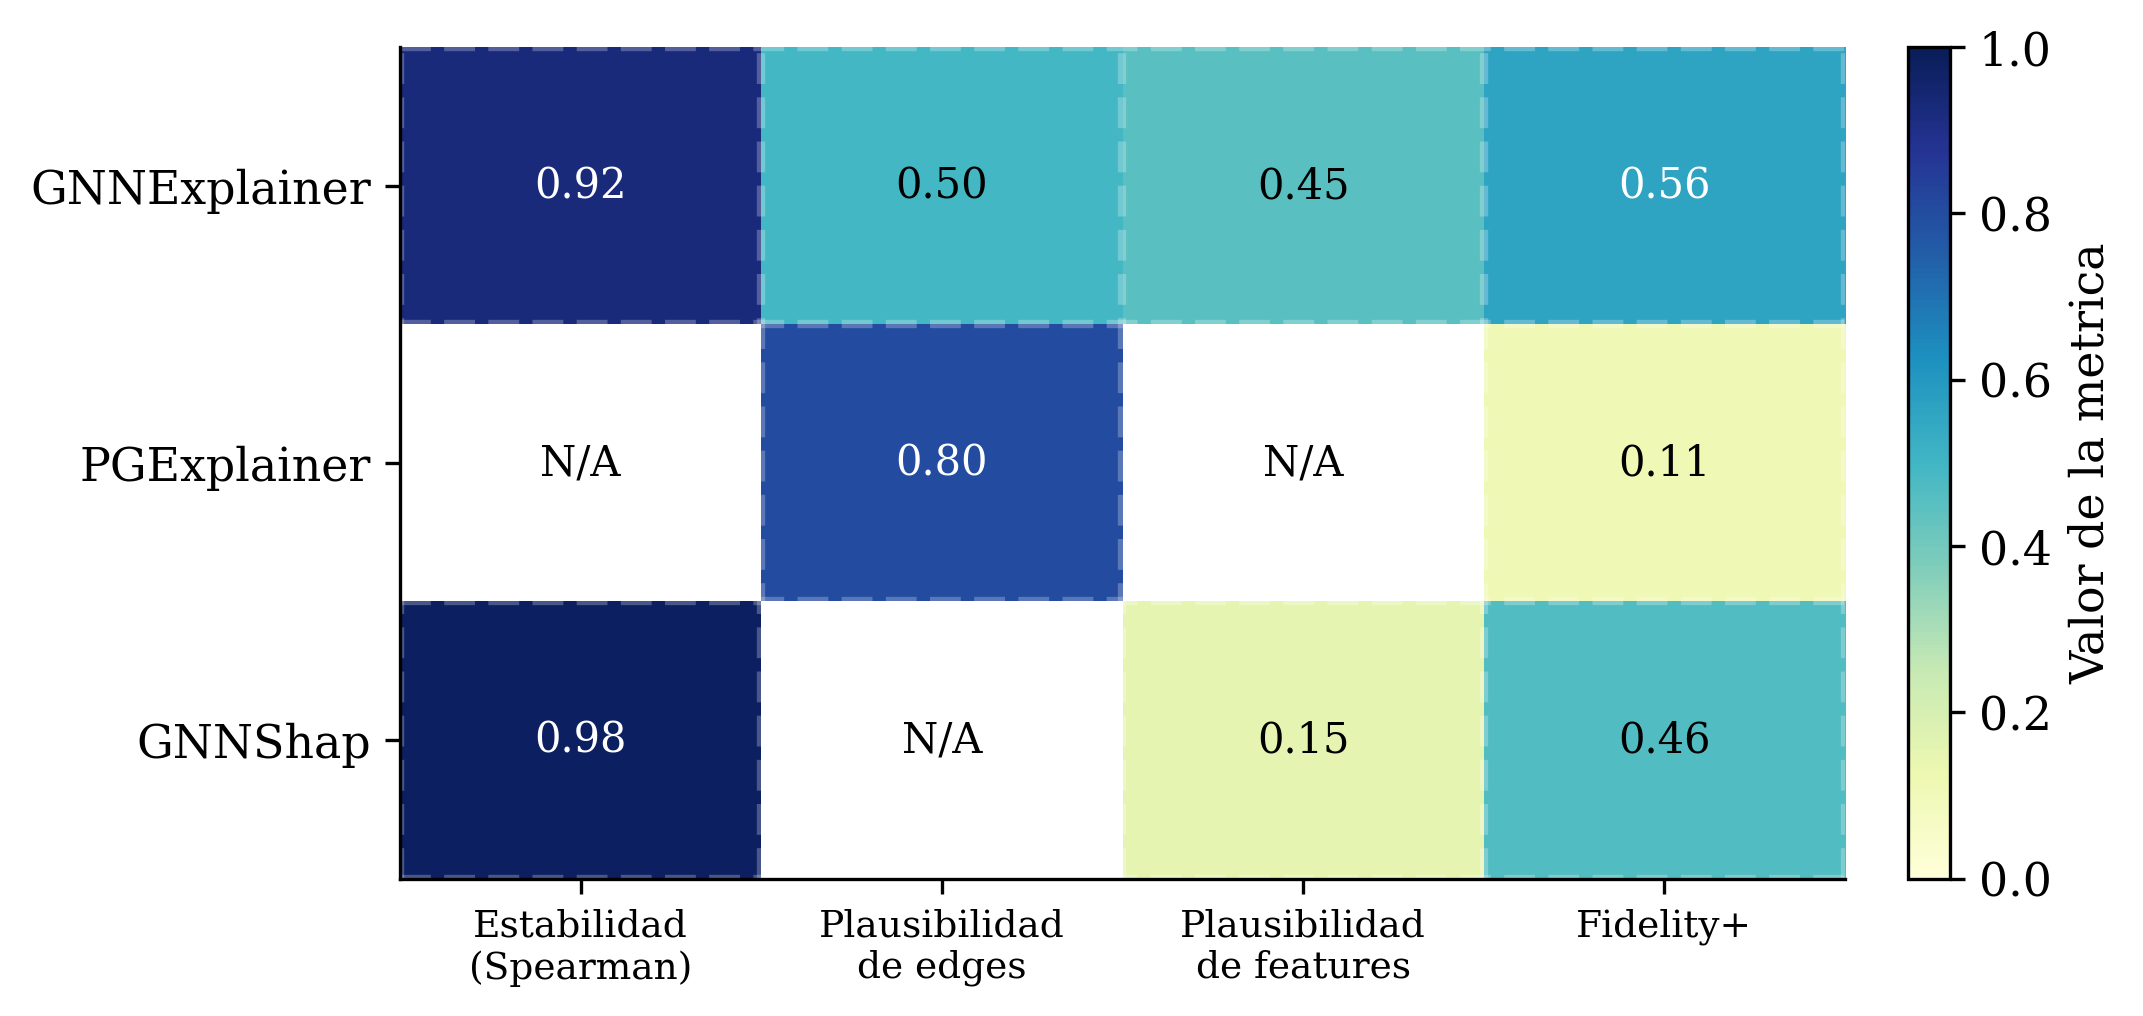
\includegraphics[width=0.95\textwidth]{chapter_5/images_ch5/heatmap_factorial.png}
    \caption{Comportamiento de los tres explicadores a través de cuatro métricas sobre el grafo sintético, promediado en la matriz factorial. Las celdas marcadas como N/A corresponden a métricas que un explicador no produce por diseño, como la estabilidad de PGExplainer, que es determinista tras entrenar, o la plausibilidad de aristas de GNNShap, que solo pondera features.}
    \label{fig:heatmap}
\end{figure}

En cuanto a la estabilidad, medida como la correlación de Spearman entre rankings de features, GNNShap resulta el más estable con un valor cercano a 0,977, por encima de GNNExplainer, que alcanza alrededor de 0,924. PGExplainer, por ser determinista una vez entrenado su modelo paramétrico, no admite una medida de estabilidad de este tipo, de modo que su celda se reporta como no aplicable. La estabilidad por arquitectura muestra un fenómeno digno de atención, ya que sobre el grafo denso GCN y GAT encabezan la estabilidad con valores cercanos a 0,965 y 0,960, con GraphSAGE y TAGCN por debajo, en torno a 0,889 y 0,886. Este orden coincide con el que arroja Elliptic una vez corregida la métrica de estabilidad, donde GCN y GAT también figuran a la cabeza, de modo que el orden de estabilidad entre arquitecturas resulta concordante entre ambos regímenes de densidad y ninguna arquitectura domina en términos absolutos. La Figura \ref{fig:contraste} contrasta directamente la estabilidad de GNNExplainer por arquitectura entre el régimen disperso de Elliptic y el régimen denso del grafo sintético, y hace visible la concordancia del orden.

\begin{figure}[htbp]
    \centering
    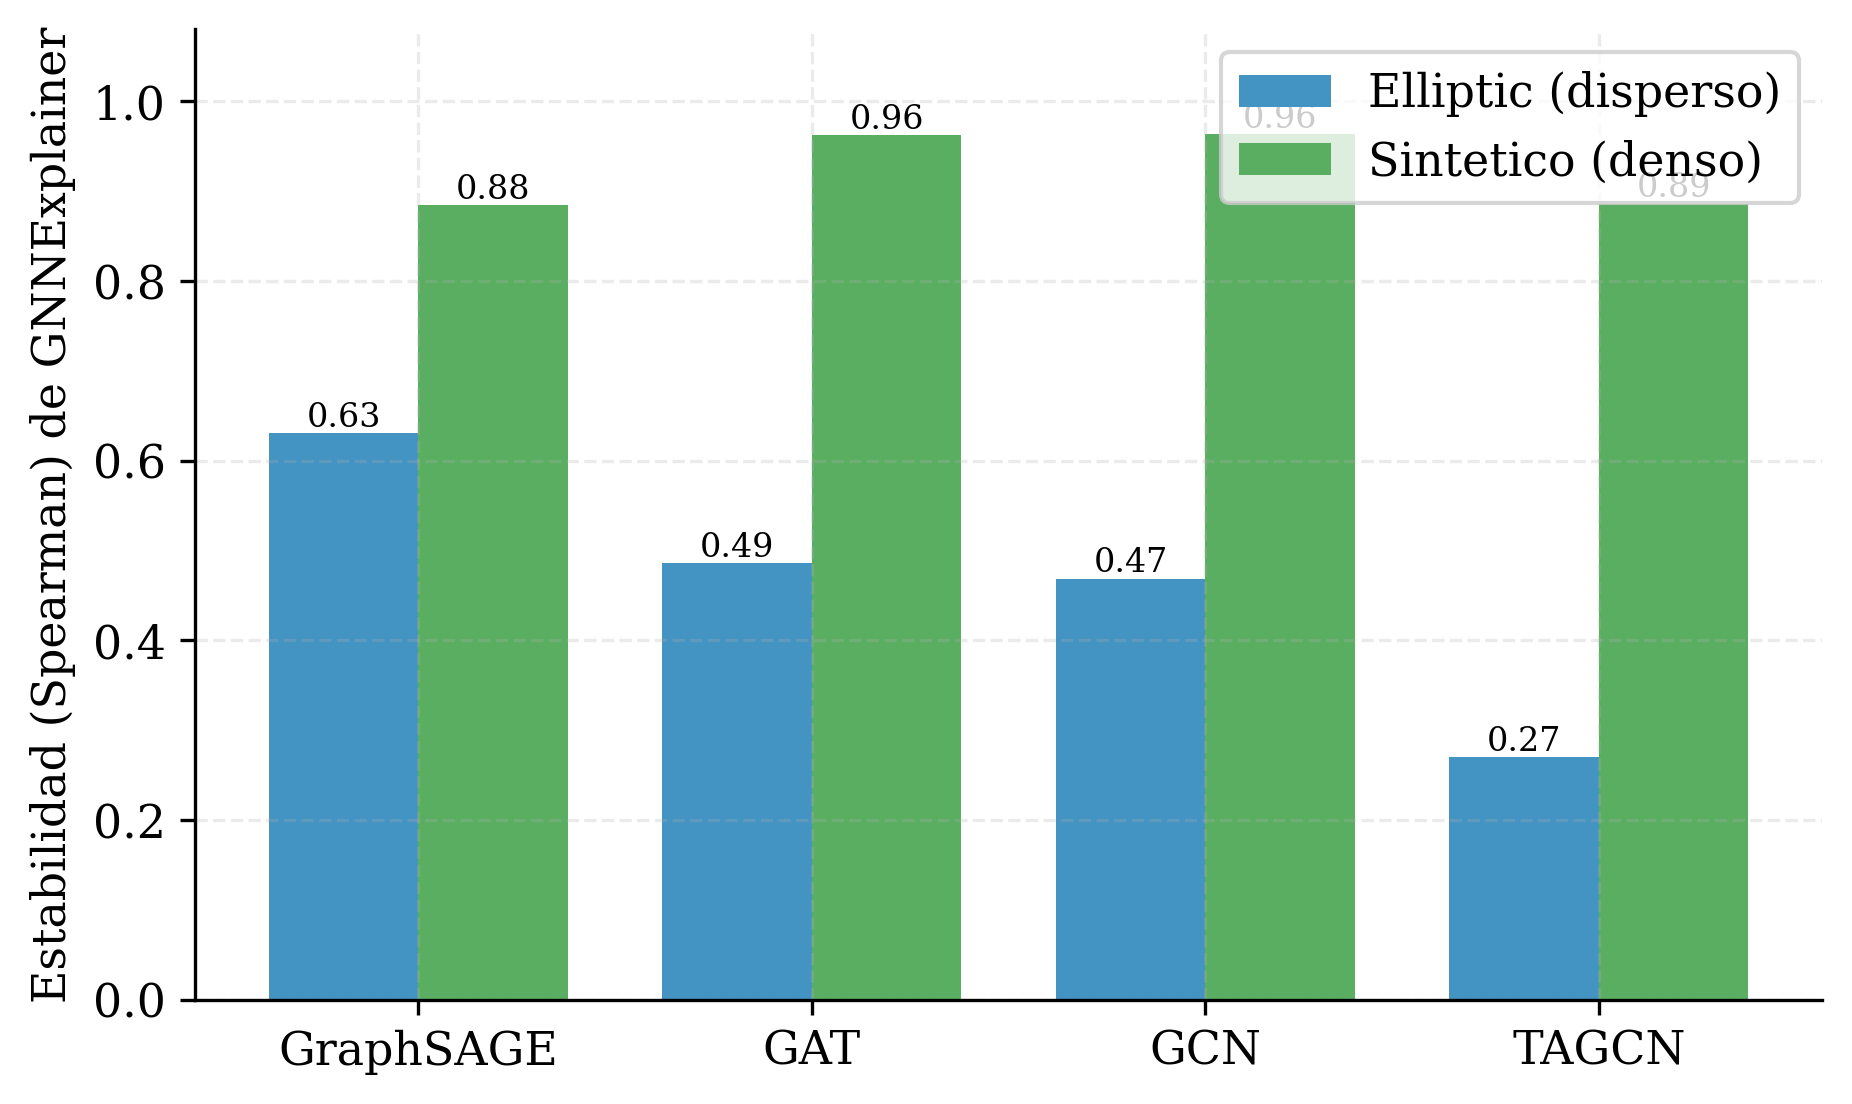
\includegraphics[width=0.85\textwidth]{chapter_5/images_ch5/contraste_regimen.png}
    \caption{Estabilidad de GNNExplainer por arquitectura en los dos regímenes de densidad. Con la métrica corregida, GCN y GAT encabezan la estabilidad tanto en el grafo disperso de Elliptic como en el grafo denso sintético, lo que evidencia que el orden de estabilidad es concordante entre regímenes y que GAT y GCN son las arquitecturas más estables con relativa independencia de la densidad.}
    \label{fig:contraste}
\end{figure}

La concordancia del orden de estabilidad entre los dos regímenes es un resultado con implicaciones conceptuales. Tanto en Elliptic, donde los vecindarios son minúsculos, como en el grafo denso sintético, GCN y GAT encabezan la estabilidad de las explicaciones, mientras que GraphSAGE y TAGCN quedan por debajo. La correlación de rangos de Spearman entre el orden de las cuatro arquitecturas en ambos regímenes cuantifica esta concordancia, ya que asciende a +0,80 con la métrica corregida, frente a -0,20 con la métrica defectuosa anterior, de modo que la reparación transforma una aparente inversión en una concordancia clara entre regímenes de densidad. Esto sugiere que la estabilidad de las explicaciones responde más al mecanismo de agregación de cada arquitectura que a la densidad del grafo sobre el que opera. Una recomendación de arquitectura orientada a la estabilidad, por tanto, parece transferirse entre regímenes de densidad distintos, si bien el reducido soporte de configuraciones con calidad garantizada en Elliptic obliga a confirmar esa transferencia con más datos antes de elevarla a regla general.

La plausibilidad revela el resultado más llamativo del eje sintético. En la plausibilidad de aristas, que mide cuán bien recupera el explicador las aristas de la tipología, PGExplainer alcanza un valor cercano a 0,801, muy por encima del 0,495 de GNNExplainer, mientras que GNNShap no produce máscara de aristas y queda fuera de esta comparación. En la plausibilidad de features, en cambio, GNNExplainer lidera con alrededor de 0,453 frente al 0,150 de GNNShap, y PGExplainer no genera un ranking de features. La fidelidad positiva, que mide cuánto cae la predicción al retirar los elementos que el explicador considera importantes, ordena a los tres métodos de otra manera, con GNNExplainer a la cabeza en torno a 0,561, GNNShap en 0,465 y PGExplainer muy por debajo, en valores de 0,110. Adicionalmente, la concentración de las atribuciones de GNNShap, medida contra el \textit{ground-truth}, alcanza un valor de 0,947, lo que ofrece una referencia cuantitativa para una métrica que en la literatura previa había quedado sin fundamento verificable. El detalle numérico completo por arquitectura y explicador se recoge en la Tabla \ref{tab:synth-factorial}, que confirma que ningún explicador domina simultáneamente en las cuatro métricas.

\begin{table}[htbp]
\centering
\renewcommand{\arraystretch}{1.3}
\small
\begin{tabular}{ll cccc}
\toprule
\textbf{Arquitectura} & \textbf{Explicador} & \textbf{Estab.} & \textbf{Plaus. aristas} & \textbf{Plaus. feat.} & \textbf{Fidelity+} \\
\midrule
GraphSAGE & GNNExplainer & 0,89 & 0,49 & 0,41 & 0,63 \\
GraphSAGE & PGExplainer & n/d & 0,92 & n/d & 0,13 \\
GraphSAGE & GNNShap & 0,97 & n/d & 0,19 & 0,55 \\
\midrule
GAT & GNNExplainer & 0,96 & 0,54 & 0,42 & 0,52 \\
GAT & PGExplainer & n/d & 0,68 & n/d & 0,12 \\
GAT & GNNShap & 0,97 & n/d & 0,18 & 0,43 \\
\midrule
GCN & GNNExplainer & 0,96 & 0,52 & 0,62 & 0,54 \\
GCN & PGExplainer & n/d & 0,73 & n/d & 0,12 \\
GCN & GNNShap & 0,99 & n/d & 0,15 & 0,51 \\
\midrule
TAGCN & GNNExplainer & 0,89 & 0,43 & 0,38 & 0,55 \\
TAGCN & PGExplainer & n/d & 0,86 & n/d & 0,07 \\
TAGCN & GNNShap & 0,97 & n/d & 0,09 & 0,37 \\
\bottomrule
\end{tabular}
\caption{Resultados de la matriz factorial sintetica por arquitectura y explicador (media sobre 3 semillas de modelo, grafo g0). Los valores n/d corresponden a metricas que un explicador no produce por diseno. Fidelity+ se calcula con la definicion manual uniforme (caida de probabilidad al retirar el top-k) para los tres explicadores. PGExplainer domina la plausibilidad de aristas, GNNExplainer la de features y la fidelidad, y GNNShap la estabilidad.}
\label{tab:synth-factorial}
\end{table}


Un resultado del eje sintético merece destacarse por su contraste con el Capítulo 4. Mientras que en Elliptic PGExplainer degeneraba de forma casi universal y producía una correlación nula, sobre el grafo denso PGExplainer no solo funciona, sino que se convierte en el explicador más plausible en aristas. Este contraste responde una pregunta metodológica que Elliptic dejaba abierta, la de si la degeneración de PGExplainer era un defecto del método o una consecuencia de la dispersión del dato. La evidencia del eje sintético indica claramente lo segundo, ya que con estructura de subgrafo suficiente PGExplainer recupera el patrón mejor que cualquier otro método, de modo que su fracaso en Elliptic se atribuye a la dispersión y no a una limitación intrínseca del explicador.

\section{Análisis Estadístico de Robustez}

Afirmar que una diferencia entre arquitecturas o entre explicadores es real exige separar la señal del ruido de una única inicialización, y la matriz factorial descrita hasta aquí entrenaba un solo modelo por celda, lo que no permitía esa separación. Para dotar de potencia inferencial al análisis, cada celda se replicó con tres semillas de modelo distintas, que producen entrenamientos independientes sobre los mismos datos, de manera que la variación entre semillas cuantifica cuánto de un resultado es atribuible al azar del entrenamiento. Esta replicación eleva la matriz a 540 filas sobre el grafo principal y se complementa con dos grafos adicionales generados con semillas distintas, para verificar que los hallazgos no dependen de una realización particular del generador. La dispersión entre semillas resultó muy baja, con una desviación típica de la correlación de Spearman media de apenas 0,007, lo que indica que los resultados son altamente reproducibles.

Esta baja dispersión tiene una lectura que va más allá de la reproducibilidad técnica. Un valor de estabilidad que apenas varía entre entrenamientos independientes indica que la propiedad medida es del método y del dato, y no de una inicialización afortunada, lo que otorga a las comparaciones entre explicadores una base firme. Sin esta verificación, cualquier diferencia observada entre dos explicadores podría atribuirse al azar de un único entrenamiento, y las conclusiones carecerían de respaldo. La replicación por semillas de modelo es, por tanto, lo que transforma un conjunto de observaciones en evidencia sobre la que se pueden sostener afirmaciones con una medida explícita de confianza.

Un control interno confirma que esta extensión es fiel al análisis original. El corte de la matriz correspondiente a la primera semilla reproduce con exactitud los valores de la matriz factorial de una sola corrida, lo que demuestra que la replicación añade réplicas sin alterar el procedimiento subyacente. Sobre esta base replicada se aplican las pruebas estadísticas introducidas en el Capítulo 3, elegidas en función de la naturaleza de las métricas. Puesto que las métricas de estabilidad y plausibilidad viven en el intervalo de cero a uno y no cumplen el supuesto de normalidad, la prueba principal para comparar factores es la de Kruskal-Wallis, acompañada del tamaño de efecto eta cuadrado, mientras que la comparación pareada entre dos explicadores recurre a la prueba de Wilcoxon de rangos con signo.

El análisis de factores arroja un resultado nítido, el explicador es el factor que más determina el comportamiento de las explicaciones. La Tabla \ref{tab:synth-stats} recoge la prueba de Kruskal-Wallis y el tamaño de efecto eta cuadrado de cada factor sobre cada métrica, y muestra que el explicador domina la estabilidad con un valor de 0,36, la plausibilidad de aristas con 0,64 y la plausibilidad de features con 0,45, cifras que corresponden a efectos grandes. La arquitectura ejerce un efecto grande únicamente sobre la estabilidad, con un valor de 0,24, y un efecto pequeño sobre las demás métricas. El balanceo, en cambio, resulta prácticamente irrelevante para la calidad de las explicaciones, con valores de eta cuadrado inferiores a 0,02 en todas las métricas, un hallazgo con implicaciones prácticas directas, ya que sugiere que la elección de la estrategia de balanceo apenas afecta a la plausibilidad o la estabilidad de las explicaciones obtenidas. La Figura \ref{fig:balanceo} ilustra esta irrelevancia, al mostrar que las tres estrategias de balanceo producen valores casi idénticos en las tres métricas principales.

\begin{figure}[htbp]
    \centering
    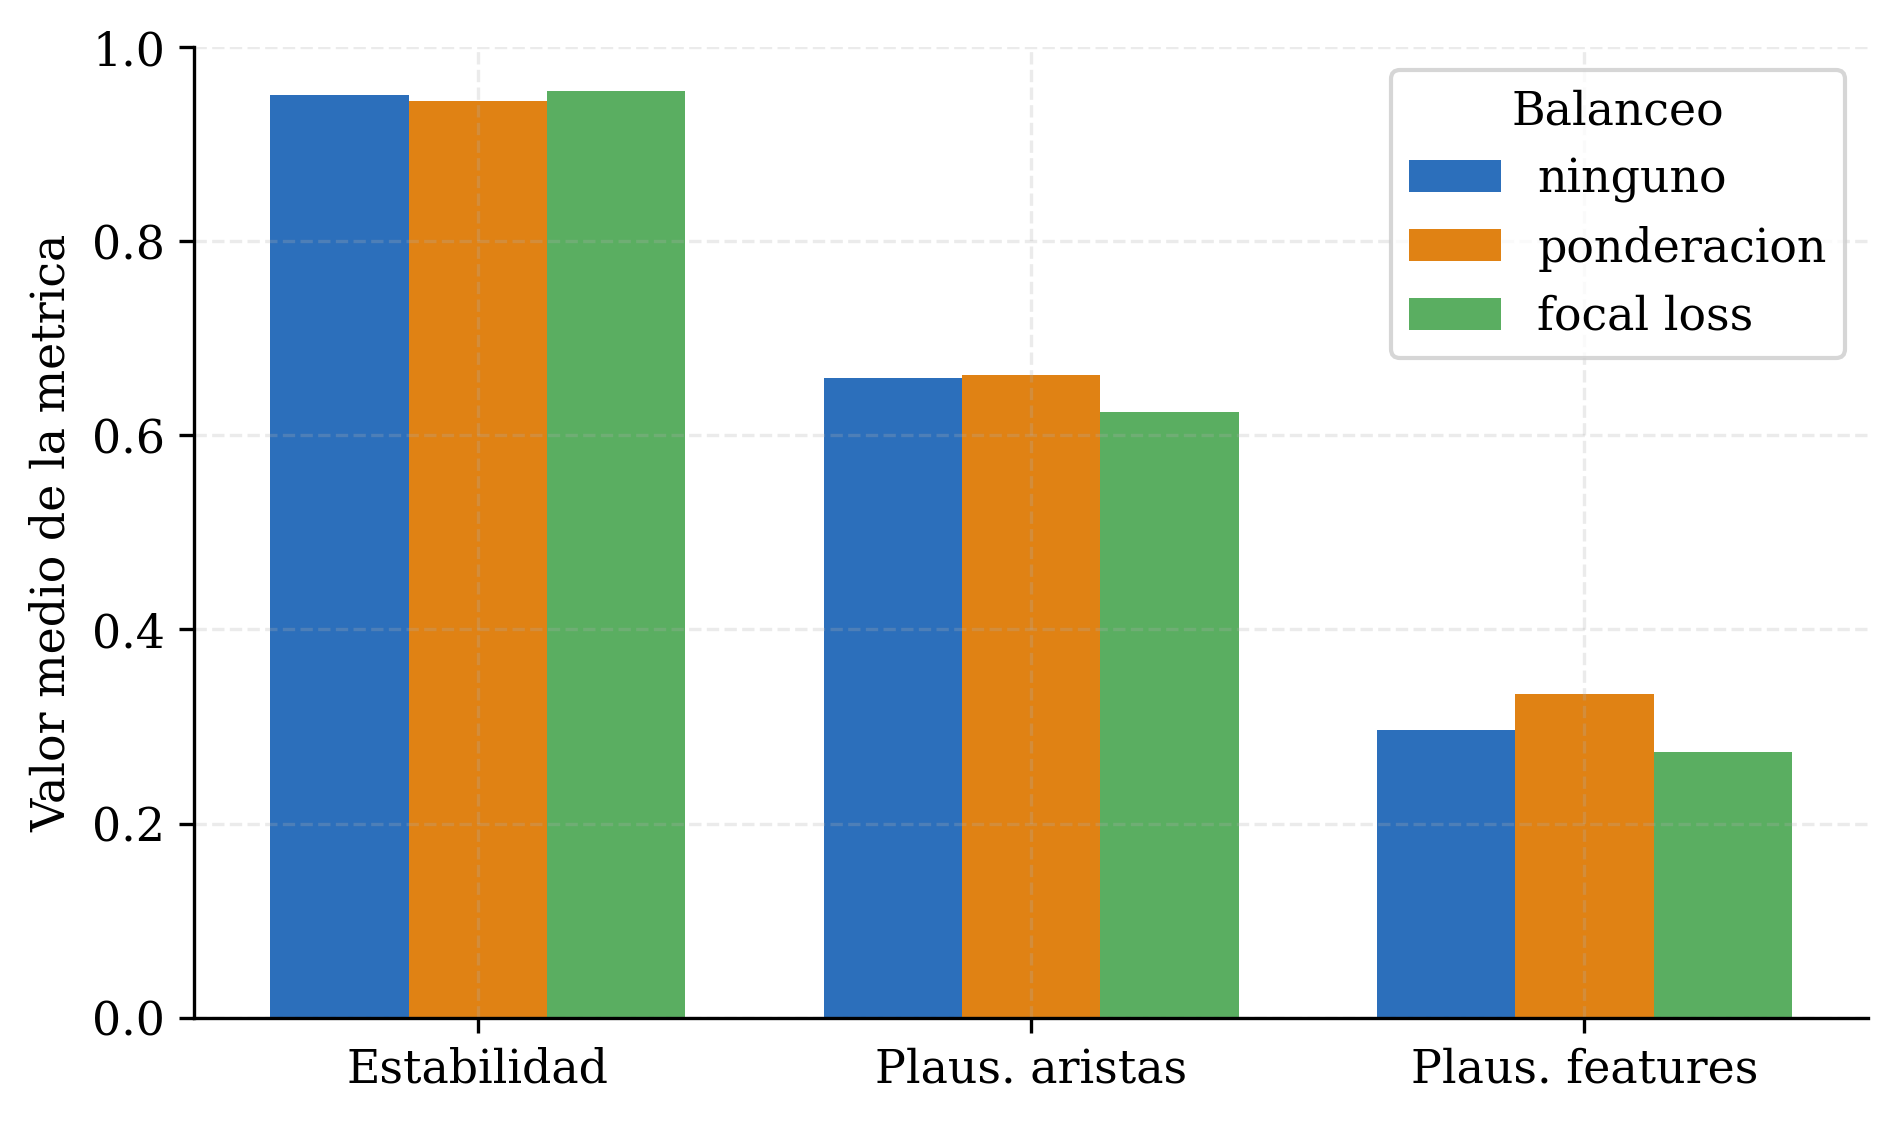
\includegraphics[width=0.85\textwidth]{chapter_5/images_ch5/balanceo_irrelevante.png}
    \caption{Estabilidad y plausibilidad medias por estrategia de balanceo sobre el grafo sintético. Las tres estrategias producen valores prácticamente indistinguibles, lo que confirma que el balanceo apenas influye en la calidad de las explicaciones.}
    \label{fig:balanceo}
\end{figure}

Este hallazgo, aunque de signo negativo, es valioso para la práctica del diseño de sistemas de detección. Buena parte del esfuerzo de diseño en escenarios con desbalance se dedica a elegir y ajustar la estrategia de balanceo, bajo la premisa de que dicha elección influye en el comportamiento del modelo y de sus explicaciones. Los resultados indican que, al menos en lo que respecta a la calidad de las explicaciones sobre un grafo con \textit{ground-truth}, esa premisa no se sostiene, y que la ponderación de clases y la Focal Loss producen explicaciones de calidad equivalente a la del entrenamiento sin intervención. La consecuencia práctica es que la estrategia de balanceo puede elegirse en función del rendimiento predictivo, sin temor a degradar de forma apreciable la interpretabilidad del modelo.

\begin{table}[htbp]
\centering
\renewcommand{\arraystretch}{1.3}
\small
\begin{tabular}{ll ccc}
\toprule
\textbf{Métrica} & \textbf{Factor} & \textbf{Kruskal-Wallis H} & \textbf{valor p} & \textbf{$\eta^2$} \\
\midrule
Estabilidad & arquitectura & 91,1 & $<$0,0001 & 0,24 \\
Estabilidad & explicador & 125,6 & $<$0,0001 & 0,36 \\
Estabilidad & balanceo & 9,1 & 0,0107 & 0,01 \\
Estabilidad & escenario & 9,9 & 0,0423 & 0,04 \\
\midrule
Plaus. aristas & arquitectura & 10,5 & 0,0149 & 0,04 \\
Plaus. aristas & explicador & 195,8 & $<$0,0001 & 0,64 \\
Plaus. aristas & balanceo & 2,4 & 0,3081 & 0,01 \\
Plaus. aristas & escenario & 2,6 & 0,6268 & 0,01 \\
\midrule
Plaus. features & arquitectura & 11,3 & 0,0103 & 0,05 \\
Plaus. features & explicador & 176,2 & $<$0,0001 & 0,45 \\
Plaus. features & balanceo & 3,5 & 0,1730 & 0,01 \\
Plaus. features & escenario & 3,0 & 0,5660 & 0,01 \\
\bottomrule
\end{tabular}
\caption{Prueba de Kruskal-Wallis y tamaño de efecto de cada factor sobre cada métrica en el grafo sintético. El estadístico H corresponde a la prueba no paramétrica, que es la que decide la significancia, mientras que el $\eta^2$ es el tamaño de efecto del análisis de varianza sobre los mismos grupos, incluido como medida de magnitud comparable entre factores. El explicador ejerce el efecto dominante en las tres métricas, la arquitectura solo en la estabilidad, y tanto el balanceo como el escenario de desbalance resultan despreciables.}
\label{tab:synth-stats}
\end{table}


El hallazgo central del eje sintético es la superioridad de PGExplainer sobre GNNExplainer en la plausibilidad de aristas, y la replicación permite comprobar si esa superioridad sobrevive a la variabilidad entre modelos. La comparación se realiza celda por celda mediante la prueba de Wilcoxon de rangos con signo, sobre 225 parejas formadas por cada combinación de grafo, arquitectura, escenario, balanceo y semilla. La diferencia media a favor de PGExplainer es de 0,299 y resulta positiva en el noventa y dos por ciento de las parejas, con un valor de significancia de 2,6 por diez elevado a menos treinta y cinco, como ilustra la Figura \ref{fig:estrella}. La superioridad se mantiene en los tres grafos generados, con valores de plausibilidad de aristas de PGExplainer de 0,820, 0,765 y 0,829, siempre por encima de los valores de GNNExplainer, según recoge la Tabla \ref{tab:grafos}. Este hallazgo, por tanto, no es un artefacto de un único entrenamiento ni de una única realización del grafo, sino un efecto sostenido y estadísticamente sólido.

Conviene preguntarse por qué PGExplainer recupera el patrón de la tipología mejor que GNNExplainer sobre el grafo denso. Una explicación plausible reside en la naturaleza amortizada de PGExplainer, que aprende un modelo paramétrico sobre todo el grafo y, por tanto, captura regularidades compartidas entre los subgrafos de una misma tipología, en lugar de optimizar una máscara de forma aislada para cada nodo. Al aprender de muchos ejemplos, el modelo paramétrico identifica qué configuraciones de aristas son características del patrón, lo que le permite señalar las aristas de la tipología con mayor precisión. GNNExplainer, en cambio, al optimizar cada explicación por separado, carece de esta capacidad de generalización entre nodos, lo que podría explicar su menor plausibilidad de aristas. Esta interpretación es coherente con el hecho de que la ventaja de PGExplainer se sostenga a través de escenarios y de grafos, ya que refleja una propiedad estructural del método y no una casualidad de una configuración particular.

La robustez del hallazgo a través de los escenarios de desbalance queda ilustrada en la Figura \ref{fig:plaus-esc}, que muestra la plausibilidad de aristas de ambos explicadores a lo largo de los cinco escenarios. La ventaja de PGExplainer se mantiene prácticamente constante con independencia del nivel de desbalance, lo que confirma que su superioridad no es un efecto de una proporción de clases particular, sino una propiedad estable del método sobre el grafo denso. Este comportamiento contrasta con la intuición inicial de que el desbalance degradaría la calidad de las explicaciones, y refuerza la conclusión de que el explicador, y no el escenario de desbalance, es el factor determinante de la plausibilidad.

\begin{figure}[htbp]
    \centering
    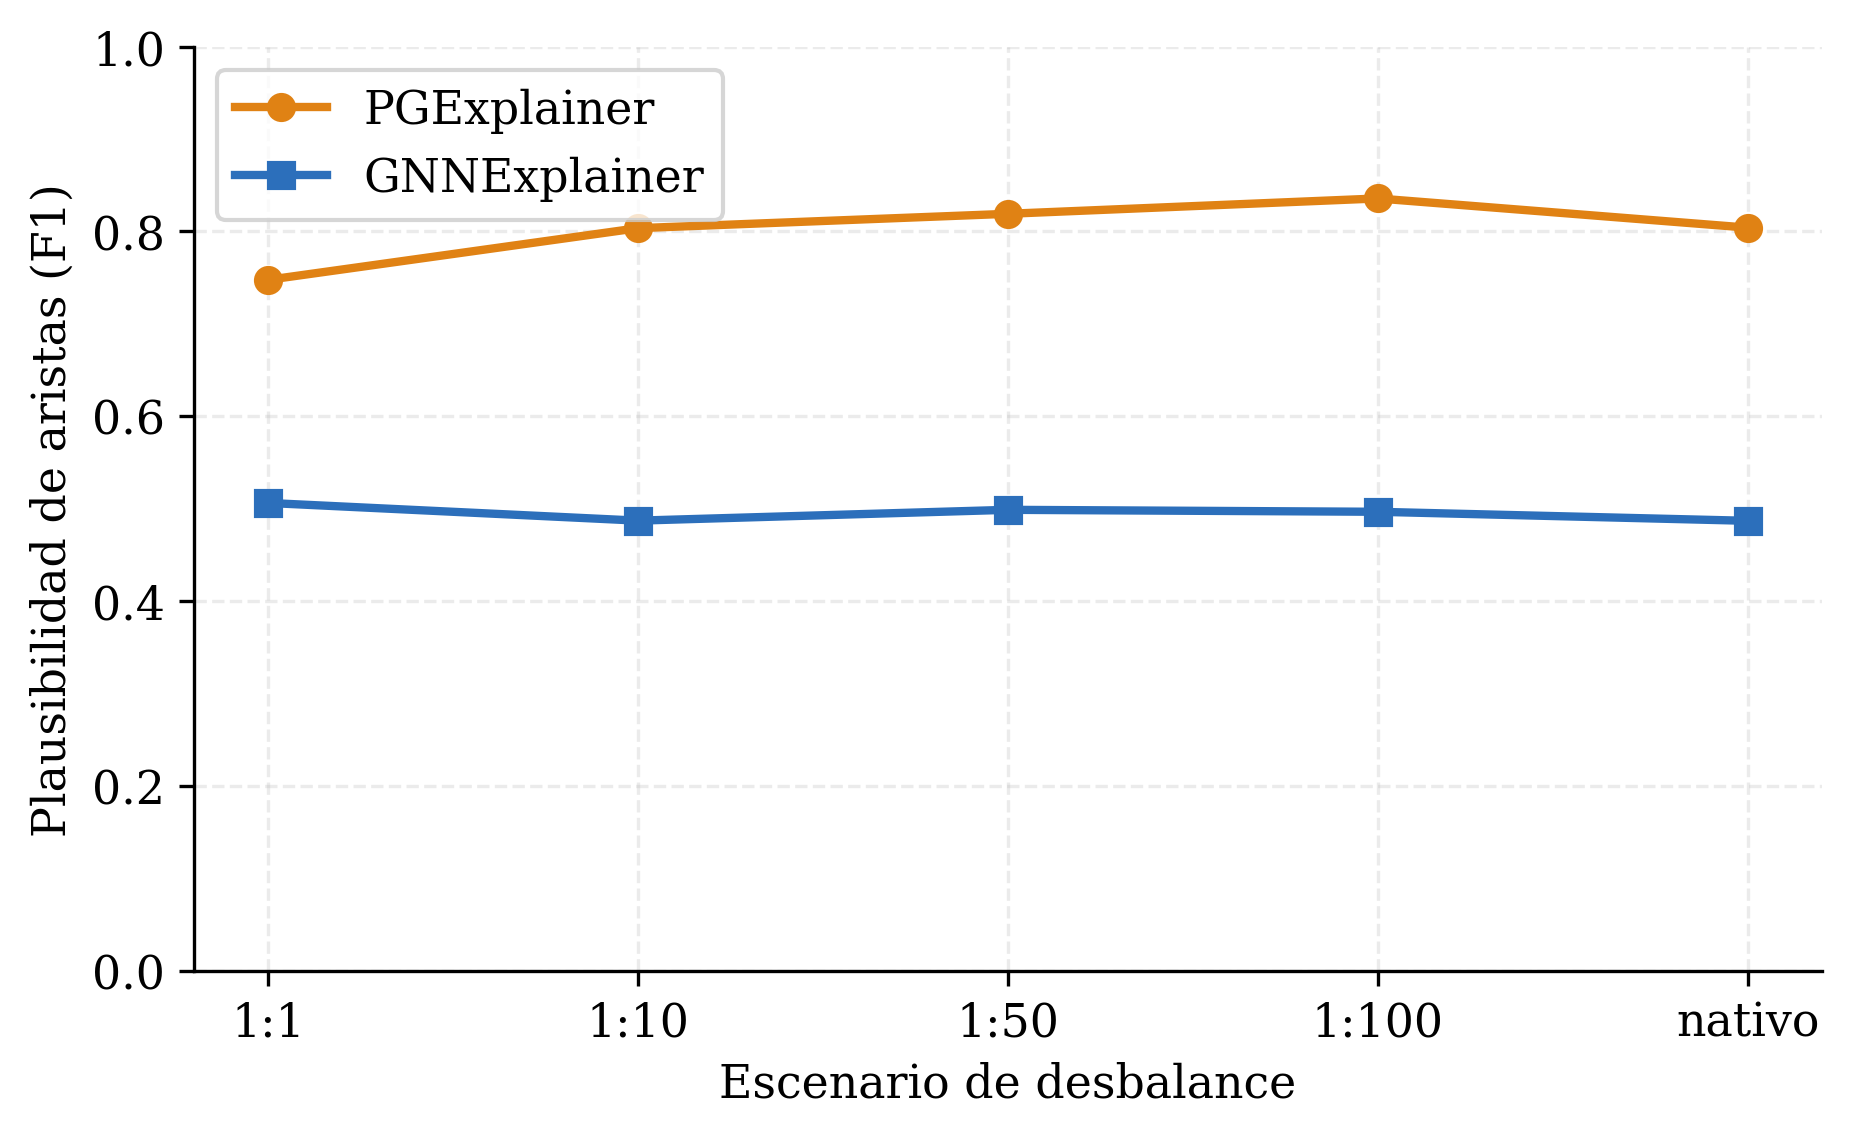
\includegraphics[width=0.8\textwidth]{chapter_5/images_ch5/plaus_escenario.png}
    \caption{Plausibilidad de aristas de PGExplainer y GNNExplainer a lo largo de los cinco escenarios de desbalance sobre el grafo sintético. La ventaja de PGExplainer se mantiene constante con independencia del nivel de desbalance, lo que confirma la robustez del hallazgo frente a la proporción de clases.}
    \label{fig:plaus-esc}
\end{figure}

\begin{figure}[htbp]
    \centering
    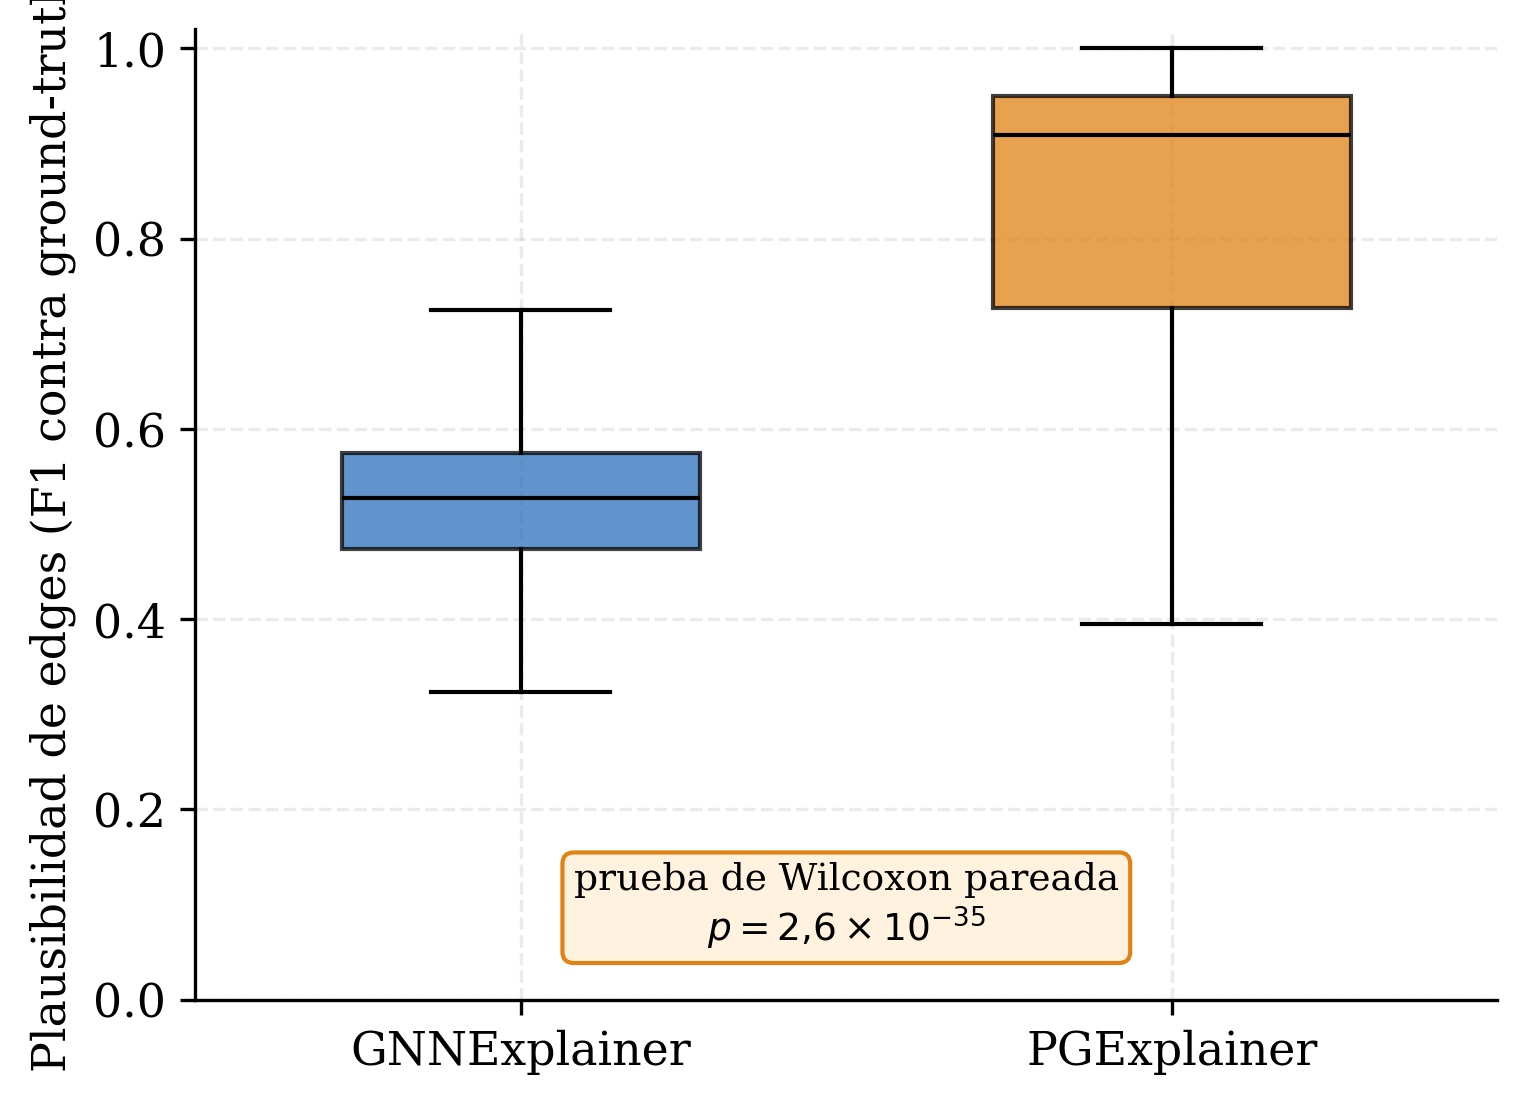
\includegraphics[width=0.6\textwidth]{chapter_5/images_ch5/hallazgo_estrella.png}
    \caption{Distribución de la plausibilidad de aristas por explicador sobre el grafo sintético. PGExplainer recupera las aristas de la tipología con una plausibilidad claramente superior a la de GNNExplainer, una diferencia confirmada por la prueba de Wilcoxon pareada.}
    \label{fig:estrella}
\end{figure}

\begin{table}[htbp]
    \centering
    \renewcommand{\arraystretch}{1.3}
    \begin{tabular}{lccc}
    \toprule
    \textbf{Explicador} & \textbf{Grafo 0} & \textbf{Grafo 1} & \textbf{Grafo 2} \\
    \midrule
    PGExplainer  & 0,801 & 0,765 & 0,829 \\
    GNNExplainer & 0,495 & 0,523 & 0,529 \\
    \bottomrule
    \end{tabular}
    \caption{Plausibilidad de aristas de PGExplainer y GNNExplainer en las tres realizaciones del grafo sintético. La superioridad de PGExplainer se mantiene en las tres instancias, lo que confirma que el hallazgo no depende de una realización particular.}
    \label{tab:grafos}
\end{table}

\section{La Ausencia de un Puente entre Estabilidad y Plausibilidad}

Una hipótesis natural, presente de forma implícita en buena parte de la literatura, sostiene que una explicación más estable debería ser también más plausible, bajo la intuición de que la consistencia entre ejecuciones reflejaría un acierto sobre el patrón real. El eje sintético permite contrastar esta hipótesis de forma directa, correlacionando la estabilidad de cada explicación con su plausibilidad, y el resultado es un puente nulo. Para GNNExplainer, la correlación entre estabilidad y plausibilidad de features es de -0,014, con un intervalo de confianza al noventa y cinco por ciento que va de -0,038 a 0,011 y que, por tanto, incluye el cero, como muestra la Figura \ref{fig:puente}. Para GNNShap, la correlación es de 0,034 con un intervalo de 0,013 a 0,053, distinguible del cero solo por el tamaño de la muestra y de una magnitud tan pequeña que carece de significado práctico, ya que explica alrededor del uno por mil de la variabilidad.

\begin{figure}[htbp]
    \centering
    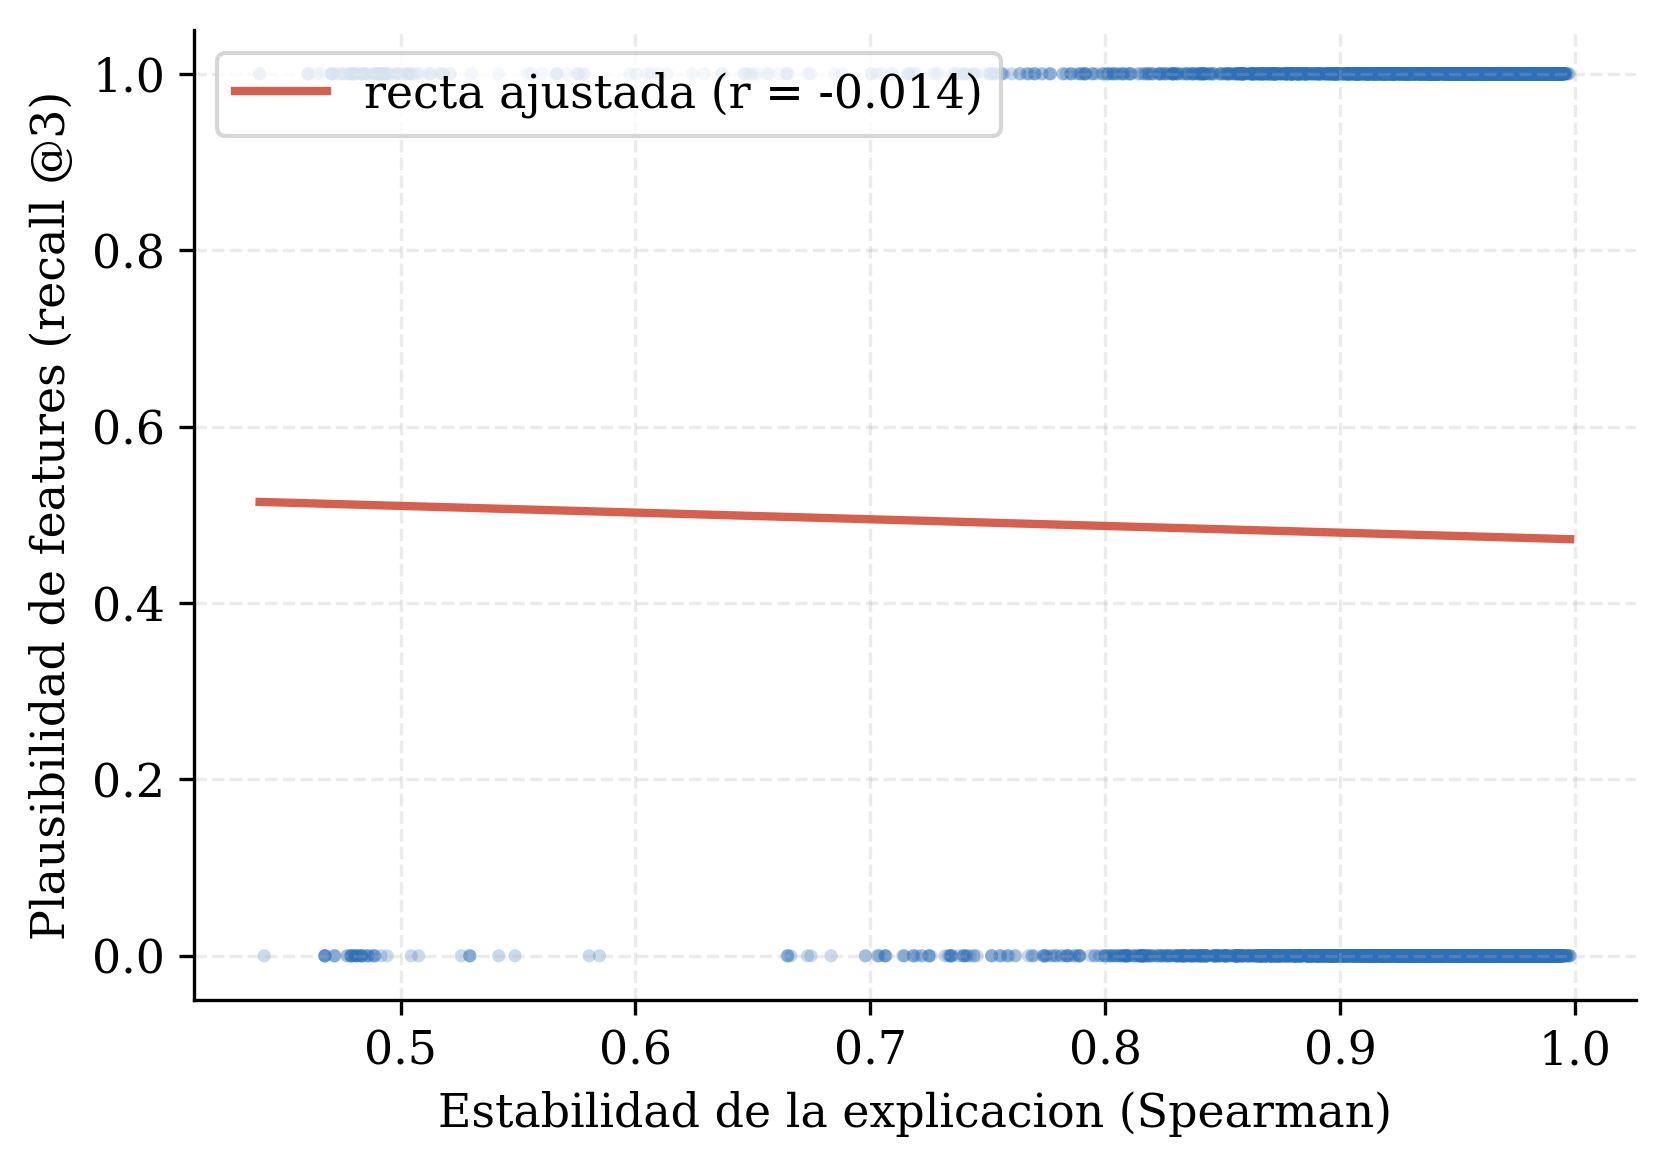
\includegraphics[width=0.7\textwidth]{chapter_5/images_ch5/puente_nulo.png}
    \caption{Relación entre la estabilidad de las explicaciones y su plausibilidad de features para GNNExplainer sobre el grafo sintético. La recta ajustada es prácticamente plana y la correlación de -0,014 no se distingue de cero, lo que evidencia la ausencia de una ley que ligue estabilidad con plausibilidad.}
    \label{fig:puente}
\end{figure}

El análisis por tipología confirma que no existe una ley universal que ligue ambas dimensiones, ya que el signo de la relación cambia según la tipología considerada. En las tipologías \textit{structuring} y \textit{fan-out} la correlación entre estabilidad y plausibilidad de aristas es positiva, con valores de 0,344 y 0,307, mientras que en \textit{layering} es negativa, con un valor de -0,102, y en \textit{fan-in} resulta nula, tal como presenta la Tabla \ref{tab:synth-bridge} junto con los intervalos de confianza bootstrap.

\begin{table}[htbp]
\centering
\renewcommand{\arraystretch}{1.3}
\begin{tabular}{lcc}
\toprule
\textbf{Tipologia} & \textbf{r (estab., aristas)} & \textbf{IC 95\%} \\
\midrule
STRUCTURING & +0,344 & [+0,301, +0,386] \\
LAYERING & -0,102 & [-0,146, -0,055] \\
FAN\_IN & -0,044 & [-0,105, +0,020] \\
FAN\_OUT & +0,307 & [+0,247, +0,362] \\
\bottomrule
\end{tabular}
\caption{Correlacion entre estabilidad y plausibilidad de aristas por tipologia para GNNExplainer, con intervalo de confianza bootstrap. El signo cambia entre tipologias, lo que confirma la ausencia de una ley universal.}
\label{tab:synth-bridge}
\end{table}
 Esta heterogeneidad, junto con el valor global cercano a cero, sostiene una conclusión clara, un explicador estable no es por ello más plausible, y ambas propiedades deben medirse por separado. Esta conclusión es coherente con las corridas previas del eje sintético, que ya habían encontrado un puente débil o nulo, y adquiere aquí un respaldo estadístico explícito mediante intervalos de confianza.

\section{La Disociación entre Plausibilidad y Fidelidad}

El análisis de la fidelidad, medida de forma uniforme para los tres explicadores, revela una tensión que la matriz factorial de una sola corrida no permitía apreciar y que constituye un hallazgo nuevo de este trabajo. PGExplainer, que es el explicador más plausible en aristas, resulta al mismo tiempo el menos fiel al modelo, con una caída de la probabilidad al retirar sus aristas de apenas 0,07 a 0,13 según la arquitectura. GNNExplainer presenta el comportamiento inverso, ya que es menos plausible pero mucho más fiel, con caídas de 0,52 a 0,63. La Figura \ref{fig:disociacion} contrasta ambas dimensiones y hace visible que la plausibilidad y la fidelidad no solo no coinciden, sino que se ordenan de manera opuesta entre estos dos explicadores.

\begin{figure}[htbp]
    \centering
    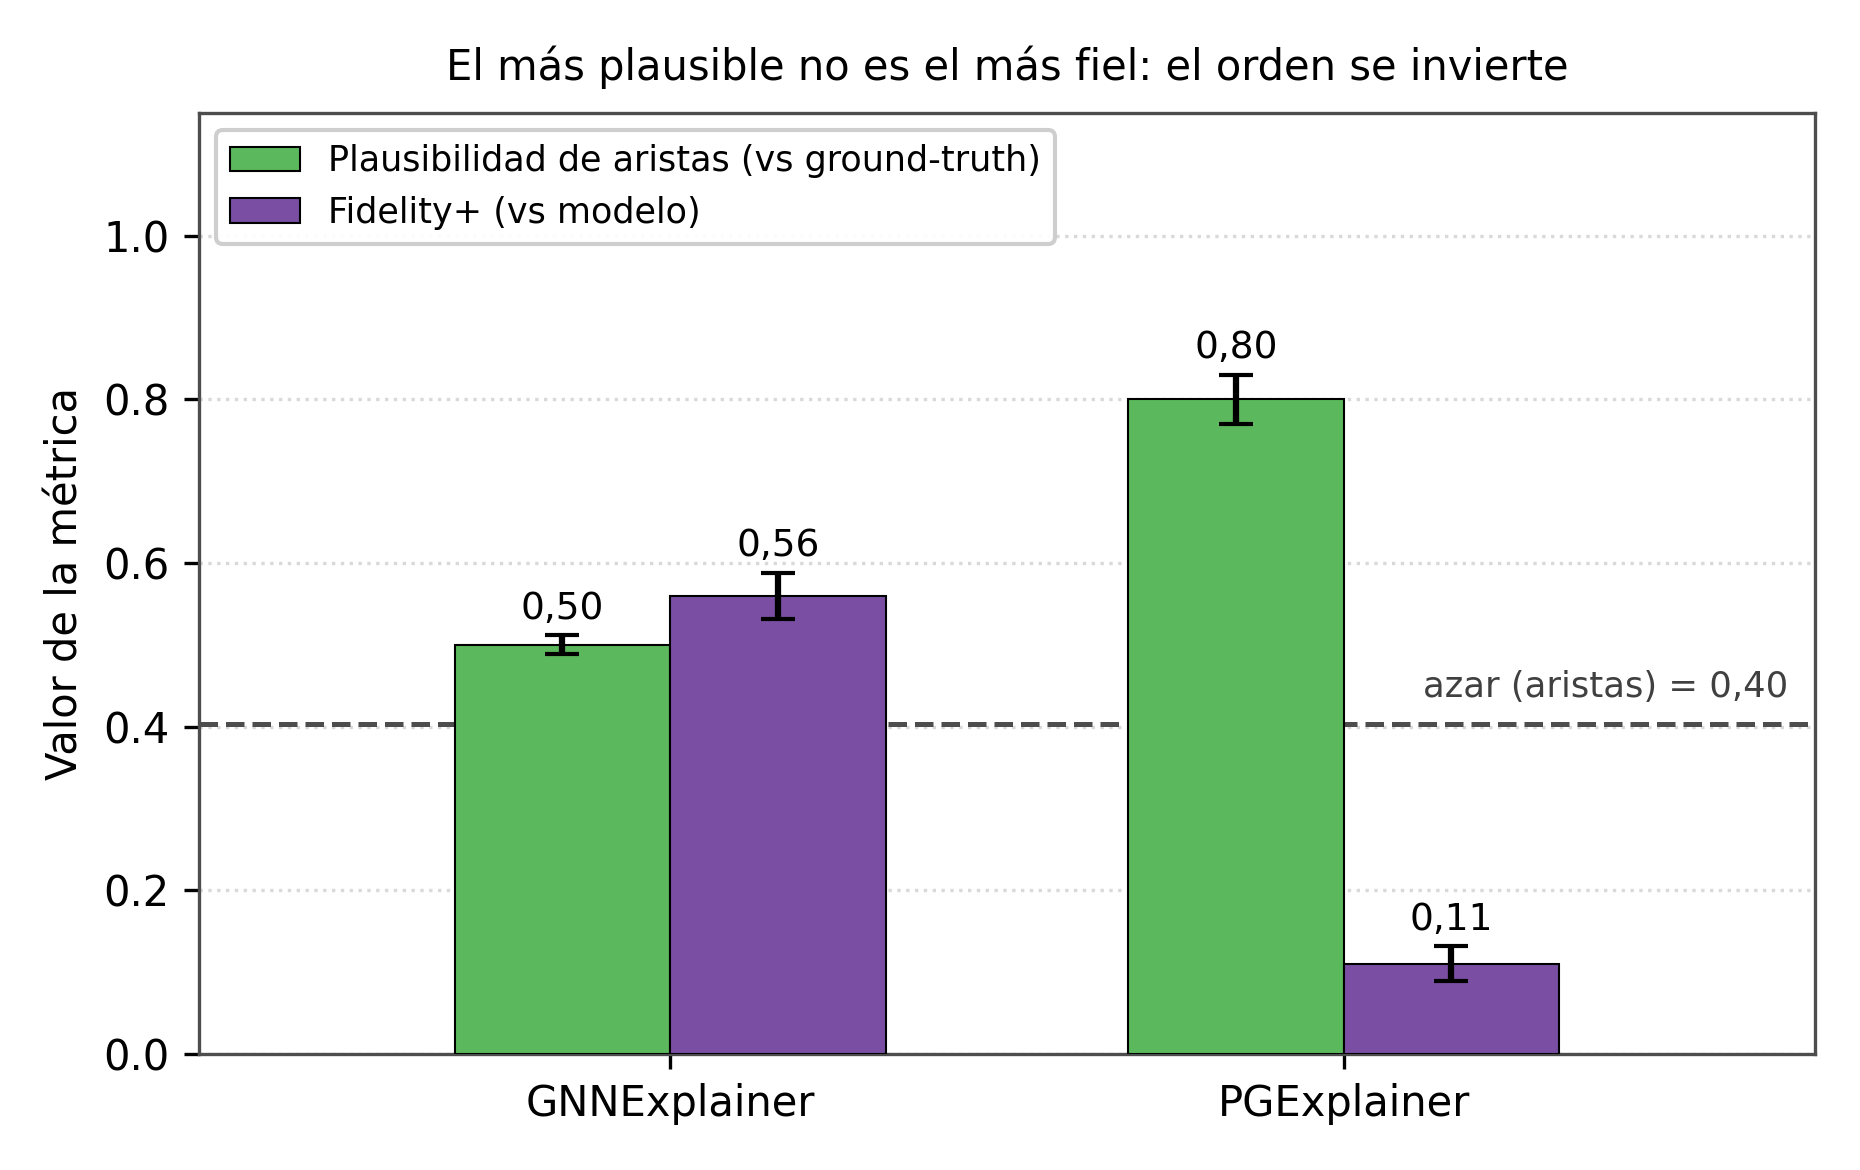
\includegraphics[width=0.85\textwidth]{chapter_5/images_ch5/disociacion.png}
    \caption{Plausibilidad frente a fidelidad positiva por explicador sobre el grafo sintético. PGExplainer es el más plausible pero el menos fiel, mientras que GNNExplainer invierte el orden, lo que evidencia la disociación entre lo que resulta plausible para un observador y lo que es fiel al mecanismo del modelo.}
    \label{fig:disociacion}
\end{figure}

La interpretación de esta disociación es a la vez sencilla y profunda. PGExplainer recupera las aristas que definen el patrón de lavado según el \textit{ground-truth}, es decir aquellas que un analista humano reconocería como la tipología, mientras que GNNExplainer recupera las aristas que el modelo realmente utiliza para decidir, y ambos conjuntos no coinciden. Dicho de otro modo, una explicación puede ser plausible, en el sentido de alinearse con el patrón que un humano considera correcto, sin ser fiel, en el sentido de reflejar el mecanismo interno del modelo, y viceversa. Esta tensión entre plausibilidad y fidelidad es un concepto conocido en la teoría de la explicabilidad, pero solo un régimen sintético con \textit{ground-truth} de tipología permite exhibirla de forma cuantitativa, ya que requiere medir simultáneamente ambas dimensiones sobre las mismas explicaciones, algo imposible en un dataset sin patrón de referencia.

La disociación tiene además una lectura práctica para quien debe elegir un explicador. Si el objetivo de una auditoría es convencer a un revisor humano de que una alerta corresponde a un patrón de lavado conocido, la plausibilidad es la propiedad relevante, y PGExplainer resulta el más adecuado pese a su baja fidelidad. Si, en cambio, el objetivo es certificar en qué se basa realmente el modelo, para detectar por ejemplo si depende de una característica espuria, la fidelidad es la propiedad relevante, y GNNExplainer resulta preferible pese a su menor plausibilidad. La imposibilidad de optimizar ambas dimensiones a la vez convierte la elección del explicador en una decisión que depende del propósito, y no en una cuestión con una única respuesta correcta. Este matiz, que la disociación hace visible, rara vez se plantea en la literatura de explicabilidad, que tiende a buscar el mejor método en abstracto.

La Figura \ref{fig:fid-arq} desglosa la fidelidad positiva por arquitectura y explicador, y confirma que el patrón de la disociación se mantiene a través de las cuatro arquitecturas. GNNExplainer conserva la fidelidad más alta en todas ellas, mientras que PGExplainer permanece en la parte baja con independencia de la arquitectura, lo que refuerza que la disociación es una propiedad del explicador y no un efecto de una arquitectura concreta.

\begin{figure}[htbp]
    \centering
    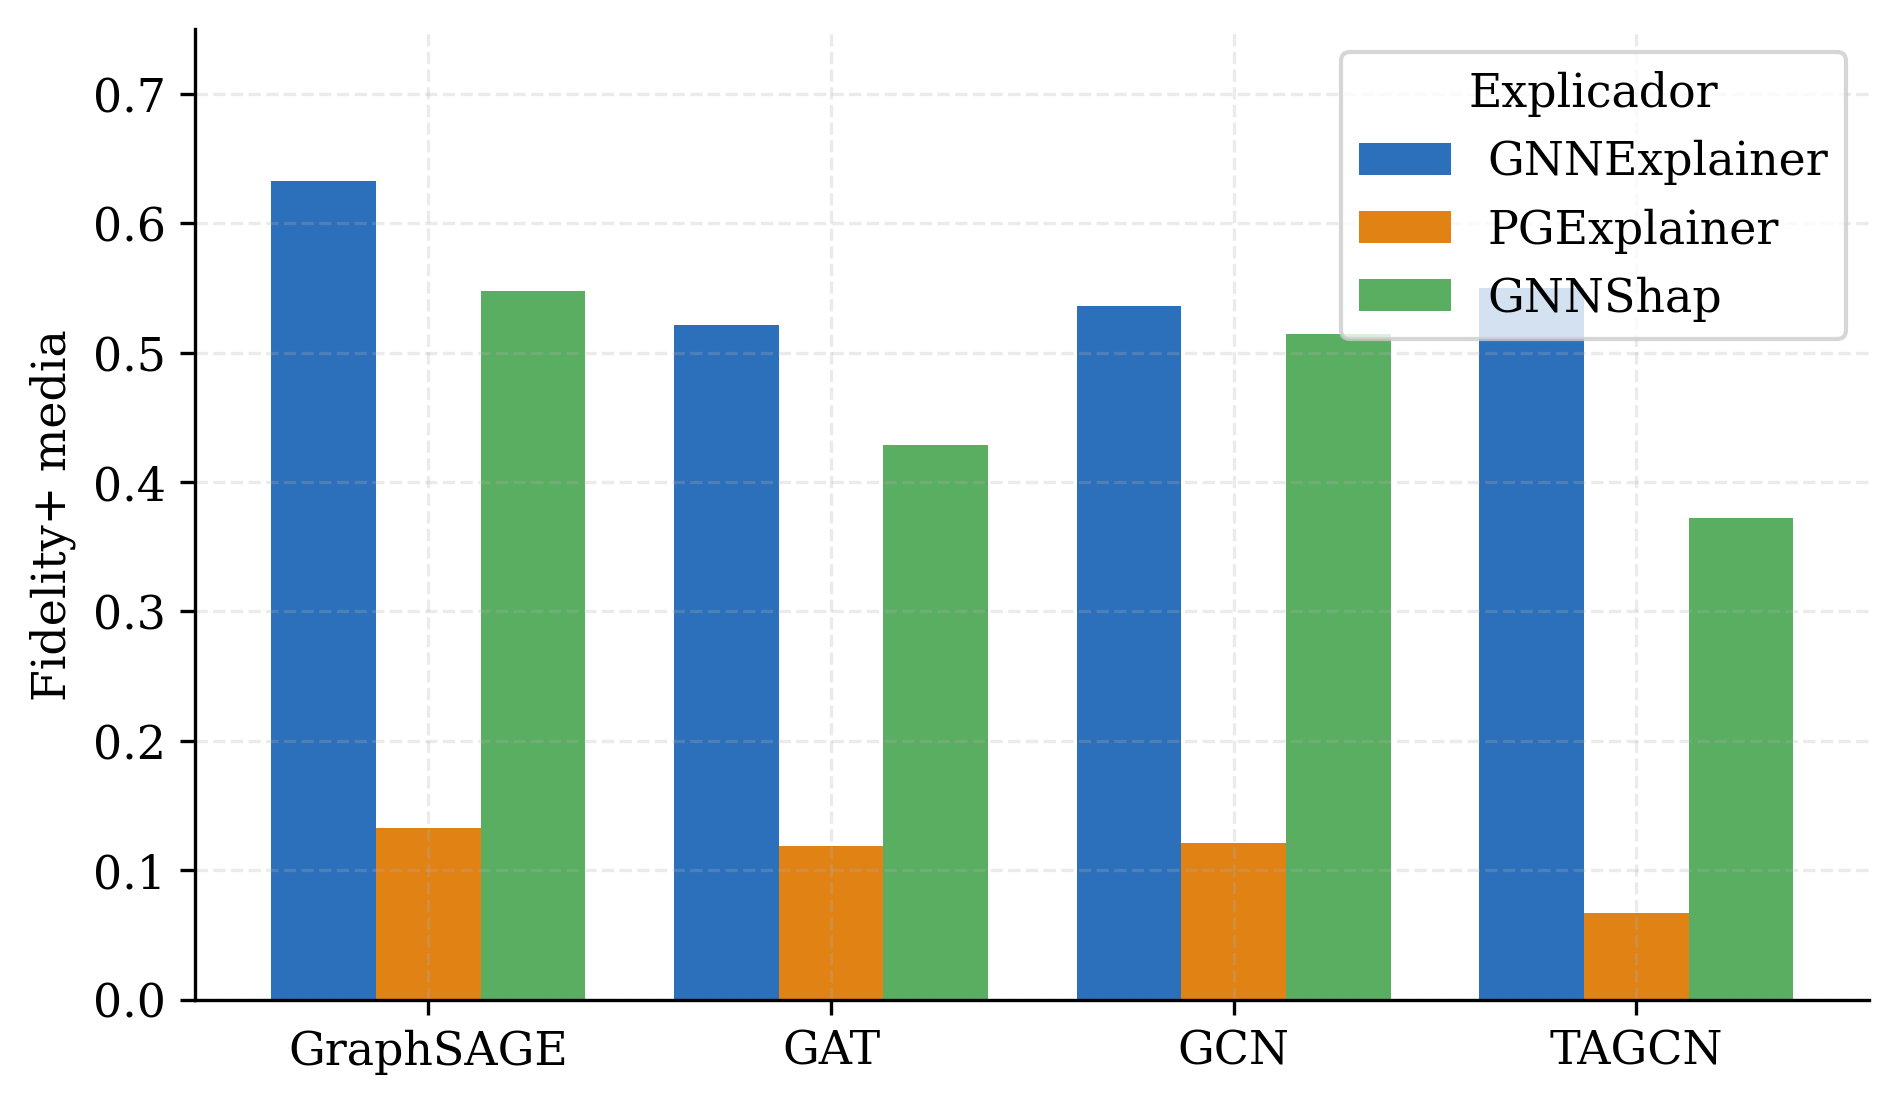
\includegraphics[width=0.85\textwidth]{chapter_5/images_ch5/fidelidad_arq.png}
    \caption{Fidelity+ media por arquitectura y explicador sobre el grafo sintético. GNNExplainer mantiene la mayor fidelidad en las cuatro arquitecturas y PGExplainer la menor, lo que confirma que la disociación entre plausibilidad y fidelidad es una propiedad del explicador y no de una arquitectura concreta.}
    \label{fig:fid-arq}
\end{figure}

\section{Síntesis del Eje Sintético}

El eje sintético cumple el propósito que motivó su construcción, medir aquello que el \textit{Elliptic Dataset} no permite y sostenerlo con un análisis estadístico riguroso. Los resultados dejan tres conclusiones que estructuran la discusión del capítulo siguiente. La primera es que el explicador es el factor determinante de la calidad de las explicaciones, muy por encima de la arquitectura y del balanceo, y que PGExplainer supera a GNNExplainer en plausibilidad de aristas de forma robusta a la variabilidad entre modelos y entre grafos. La segunda es que no existe un puente entre estabilidad y plausibilidad, de modo que un explicador estable no es por ello más acertado sobre el patrón real. La tercera es la disociación entre plausibilidad y fidelidad, que obliga a distinguir con cuidado entre una explicación que convence a un humano y una explicación que refleja el razonamiento del modelo. Más allá de estos tres hallazgos, el eje sintético demuestra la viabilidad de un enfoque de evaluación que la comunidad de explicabilidad podría adoptar de forma más amplia. Al construir un grafo con \textit{ground-truth} de tipología y densidad controlada, se obtiene un banco de pruebas en el que la plausibilidad, la fidelidad y la estabilidad de un explicador pueden medirse de forma simultánea y objetiva, algo que los conjuntos de datos reales rara vez permiten. Este enfoque no sustituye la validación sobre datos reales, pero la complementa al ofrecer un entorno en el que las afirmaciones sobre la calidad de una explicación son verificables contra una referencia conocida. La combinación de ambos tipos de evidencia, la validez externa de los datos reales y la validez interna del grafo controlado, es lo que confiere solidez a las conclusiones de esta tesis.

Estas conclusiones, junto con las del eje Elliptic, se integran y se discuten en el Capítulo 6.

\chapter{DISCUSIÓN}

Este capítulo integra los resultados de los dos ejes experimentales y examina sus implicaciones para el diseño de sistemas AML auditables. La discusión parte de la lectura conjunta de Elliptic y del grafo sintético, deriva de ella una reconsideración de qué factores gobiernan la calidad de las explicaciones, y sitúa los hallazgos frente al estado del arte. El capítulo cierra con una exposición honesta de las limitaciones del estudio, dado que reconocer sus fronteras es condición para interpretar correctamente su alcance.

\section{Lectura Conjunta de los Dos Ejes}

La combinación de los dos ejes ofrece una imagen más completa que la que cualquiera de ellos podría dar por separado, y esa complementariedad es precisamente el argumento metodológico central de la tesis. El eje Elliptic aporta el realismo de datos de Bitcoin con ruido, desbalance y desplazamiento temporal, y en él se establece, una vez corregidos dos artefactos de evaluación sucesivos y replicado el entrenamiento con tres semillas de modelo, que la estabilidad no ordena a las cuatro arquitecturas en cuatro posiciones distinguibles sino que las separa en dos grupos, uno alto formado por GAT y GCN y uno bajo formado por GraphSAGE y TAGCN, con diferencias significativas entre grupos y no dentro de ellos. El eje sintético aporta el control necesario para medir la plausibilidad, y en él se establece que el explicador es el factor determinante, que PGExplainer recupera mejor el patrón de referencia y que no existe un puente entre estabilidad y plausibilidad. Ninguno de los dos ejes contradice al otro, sino que cada uno responde preguntas que el otro no puede abordar, de modo que su lectura conjunta sostiene conclusiones más robustas que las de un diseño de un solo dataset.

Un punto de contacto entre ambos ejes merece subrayarse, el comportamiento de PGExplainer. En Elliptic, PGExplainer degeneraba de forma casi universal y producía correlaciones nulas, lo que en un estudio de un solo dataset habría llevado a concluir que se trata de un método deficiente. El eje sintético desmiente esa conclusión, ya que sobre un grafo denso PGExplainer se convierte en el explicador más plausible, lo que revela que su fracaso en Elliptic era una consecuencia de la dispersión del dato y no una propiedad del método. Este contraste ilustra el valor de disponer de dos regímenes de densidad distintos, puesto que permite distinguir entre las limitaciones de un método y las limitaciones que el dato impone a cualquier método.

\section{Estabilidad, Plausibilidad y Fidelidad como Tres Dimensiones Independientes}

El hallazgo más consecuente de la tesis es que la estabilidad, la plausibilidad y la fidelidad de una explicación son dimensiones independientes que deben medirse por separado. El puente nulo entre estabilidad y plausibilidad demuestra que un explicador consistente entre ejecuciones no acierta por ello sobre el patrón real, y la disociación entre plausibilidad y fidelidad demuestra que un explicador que recupera el patrón que un humano reconoce no refleja necesariamente el mecanismo interno del modelo. Estas dos relaciones, tomadas en conjunto, desmontan la intuición de que existe una única noción de buena explicación que las tres métricas capturarían de forma redundante. Por el contrario, cada dimensión responde a una pregunta distinta, la estabilidad pregunta si la explicación es reproducible, la plausibilidad pregunta si coincide con el conocimiento del dominio, y la fidelidad pregunta si describe lo que el modelo hace.

La independencia de estas tres dimensiones sugiere que la evaluación de explicaciones debería adoptar un enfoque multidimensional de forma sistemática. Reportar una única métrica de calidad, como es habitual en muchos trabajos, oculta compromisos que pueden ser decisivos para la aplicación. Un método que encabeza un ranking de estabilidad podría ocupar el último lugar en fidelidad, de modo que una comparación basada en una sola dimensión conduciría a una recomendación equivocada según el propósito real de la explicación. Esta tesis aboga, en consecuencia, por caracterizar cada explicador a través de las tres dimensiones de forma conjunta, y por hacer explícito el propósito de la auditoría antes de seleccionar un método.

Esta independencia tiene consecuencias directas para la práctica de la auditoría en entornos regulados. Un equipo de cumplimiento que necesite justificar una alerta ante un regulador debe decidir qué dimensión prioriza, ya que ningún explicador las optimiza todas a la vez. Si el objetivo es demostrar que la alerta responde a un patrón de lavado reconocible, la plausibilidad es la dimensión relevante y PGExplainer resulta preferible, aunque su baja fidelidad advierta que la explicación puede no coincidir con el razonamiento del modelo. Si el objetivo es auditar el modelo en sí, para verificar en qué se basa realmente su decisión, la fidelidad es la dimensión relevante y GNNExplainer resulta preferible, aunque su plausibilidad sea menor. La elección, por tanto, no es técnica sino que depende del propósito de la auditoría, una conclusión que la literatura sobre explicabilidad rara vez plantea de forma tan explícita \cite{Agarwal2022ProbingMethods, Adadi2018PeekingXAI}.

\section{El Papel Secundario del Balanceo y de la Arquitectura}

Un resultado que contrasta con parte de la literatura es el papel prácticamente nulo del balanceo sobre la calidad de las explicaciones. Trabajos previos habían sugerido que las estrategias de mitigación del desbalance influyen tanto en el clasificador como en la consistencia de las explicaciones \cite{Rai2025EvaluatingData, Fujiwara2024KnowledgeStability}. Los resultados del eje sintético, en cambio, muestran que el balanceo tiene un tamaño de efecto despreciable sobre la estabilidad y la plausibilidad, muy por debajo del efecto del explicador. Esta discrepancia puede explicarse porque los trabajos anteriores median el efecto del balanceo sobre el clasificador o sobre datos distintos de los grafos financieros, mientras que la presente tesis lo mide directamente sobre la calidad de las explicaciones en un grafo con \textit{ground-truth}, un encuadre que aísla mejor la contribución de cada factor.

La arquitectura ocupa una posición intermedia, con un efecto apreciable sobre la estabilidad pero pequeño sobre la plausibilidad. Una vez corregidos los dos artefactos de evaluación, el orden de estabilidad entre arquitecturas deja de invertirse entre Elliptic y el grafo sintético y pasa a ser concordante, con GAT y GCN a la cabeza en ambos regímenes. La replicación con tres semillas precisa el alcance de esta concordancia y la refuerza, ya que los dos regímenes no solo coinciden en qué arquitecturas encabezan, sino en la partición completa, con GAT y GCN separados de GraphSAGE y TAGCN. La separación entre los dos grupos alcanza significación estadística en ambos ejes, y dentro del grupo bajo las dos arquitecturas resultan indistinguibles también en ambos, con valores p de 0,096 en Elliptic y de 0,519 en el grafo sintético. Dentro del grupo alto la distinción depende del régimen, puesto que en Elliptic GAT y GCN no se separan mientras que en el grafo sintético GCN supera a GAT con un valor p de 0,0013, si bien por un margen de seis milésimas que carece de relevancia práctica y que solo resulta detectable por el mayor número de celdas y la menor varianza de ese eje. Que dos regímenes de densidad opuesta, medidos sobre datos distintos y con pipelines independientes, converjan en la misma partición ofrece un respaldo más fuerte que la coincidencia de un ordenamiento entre cuatro posiciones. La conclusión práctica se modifica en consecuencia, puesto que la elección de arquitectura sí ofrece una palanca de estabilidad, aunque de grano grueso, ya que lo que la evidencia sostiene es la elección de grupo y no la elección de una arquitectura concreta dentro de él.

La concordancia del orden de estabilidad entre regímenes tiene una implicación teórica que conviene explicitar, y la partición en dos grupos la vuelve más nítida de lo que permitía un ordenamiento de cuatro posiciones. La composición de los grupos no es arbitraria desde el punto de vista del mecanismo de agregación. GCN y GAT, las dos arquitecturas del grupo alto, ponderan la vecindad inmediata de forma determinista una vez fijados los parámetros, la primera mediante una normalización espectral fija y la segunda mediante pesos de atención que, aunque aprendidos, no varían en inferencia. GraphSAGE y TAGCN, las dos del grupo bajo, introducen en cambio sendas fuentes de variabilidad, ya que la primera muestrea la vecindad y la segunda reparte la importancia sobre un campo receptivo ampliado por el orden del filtro polinomial. La estabilidad de una explicación dependería, según esta lectura, de si el mecanismo de agregación concentra la atribución sobre un conjunto reducido y fijo de vecinos o la dispersa sobre un conjunto amplio o variable. Aunque esta interpretación requiere confirmación adicional, el hecho de que la misma partición emerja de forma independiente en dos regímenes de densidad opuesta le otorga un respaldo apreciable, y abre una línea de investigación sobre la relación entre la agregación y la estabilidad explicativa.

\section{Contribuciones Metodológicas}

Más allá de los hallazgos sustantivos, la tesis aporta varias contribuciones metodológicas que conviene destacar. La primera es la corrección del subgrafo receptivo, que revela cómo un fallo silencioso de memoria puede confundirse con una propiedad de una arquitectura, un riesgo general en la evaluación de explicadores que rara vez se documenta. La segunda es la distinción entre la degeneración de un método y la limitación que el dato impone, ilustrada por el comportamiento de PGExplainer en los dos regímenes de densidad. La tercera es la medición uniforme de la fidelidad para los tres explicadores, que hace posible la comparación completa que dio lugar al hallazgo de la disociación, y que suple una carencia de las implementaciones estándar, las cuales no cubren por igual a todos los métodos. La cuarta es la distinción, establecida de forma empírica al replicar el entrenamiento, entre la reproducibilidad de los pesos y la reproducibilidad de las conclusiones. Reentrenar la matriz con la misma semilla no devuelve modelos idénticos, porque las operaciones de dispersión del paso de mensajes sobre la unidad de procesamiento gráfico emplean sumas atómicas de orden no determinista, y sin embargo devuelve el mismo filtro de calidad y el mismo orden de estabilidad. Enunciar esa distinción evita tanto una expectativa de reproducibilidad exacta que el cómputo sobre aceleradores gráficos no puede satisfacer, como la conclusión opuesta y errónea de que un resultado no reproducible bit a bit carece de valor científico.

A estas contribuciones se suma una práctica de honestidad metodológica que atraviesa todo el trabajo, la de retractar conclusiones anteriores cuando la evidencia corregida las contradice. La tesis retira de forma explícita el supuesto compromiso entre exactitud y estabilidad, el supuesto pico de inestabilidad en un escenario intermedio y la supuesta paradoja del escenario nativo, porque todos ellos se apoyaban en el artefacto de memoria ya descrito. Retractar hallazgos no es un signo de debilidad, sino una manifestación del rigor que exige sustituir conclusiones apoyadas en artefactos por conclusiones apoyadas en mediciones homogéneas. Esta actitud es coherente con las advertencias de la literatura sobre la sensibilidad de los resultados de explicabilidad al protocolo experimental \cite{Kosan2023GNNX-BENCH:Benchmarking}.

\section{Relación con el Estado del Arte}

Los hallazgos de esta tesis dialogan de forma directa con varios trabajos del estado del arte, a los que confirman en algunos aspectos y matizan en otros. La distinción entre plausibilidad y fidelidad que aquí se cuantifica coincide con la advertencia teórica de Agarwal y colaboradores, quienes señalaron que muchas explicaciones consideradas plausibles no son necesariamente fieles al mecanismo del modelo \cite{Agarwal2022ProbingMethods}. La contribución de esta tesis consiste en llevar esa advertencia del plano conceptual al plano de la medición, mostrando con un grafo de \textit{ground-truth} conocido que la plausibilidad y la fidelidad no solo difieren, sino que pueden ordenarse de manera opuesta entre explicadores. De este modo, la disociación deja de ser una posibilidad teórica y se convierte en un fenómeno observado y cuantificado sobre un conjunto de datos controlado.

La sensibilidad de los resultados al protocolo de evaluación, documentada por Kosan y colaboradores mediante un \textit{benchmark} exhaustivo, encuentra en esta tesis una ilustración concreta y de consecuencias graves \cite{Kosan2023GNNX-BENCH:Benchmarking}. Los dos artefactos que alteraron el ranking de estabilidad, primero un fallo de memoria que favorecía a GAT y después un truncamiento de la métrica de Spearman que favorecía a GraphSAGE, son precisamente el tipo de dependencia del protocolo que aquel trabajo advertía, y su corrección sucesiva demuestra que un detalle de implementación puede determinar por completo la conclusión de un estudio comparativo. Este episodio refuerza la necesidad de auditar tanto los métodos como las condiciones de cómputo bajo las que se miden. La coincidencia entre una advertencia general de la literatura y un caso concreto en este estudio otorga a la corrección un valor que trasciende el resultado puntual.

La relación con los trabajos sobre desbalance y explicabilidad merece un comentario cuidadoso. Rai y colaboradores junto con Fujiwara reportaron que el desbalance de clases afecta a la consistencia de las explicaciones \cite{Rai2025EvaluatingData, Fujiwara2024KnowledgeStability}. Los resultados de esta tesis no contradicen esa observación en cuanto al clasificador, pero sí matizan su alcance sobre la calidad de las explicaciones, ya que el balanceo, medido de forma aislada sobre un grafo con \textit{ground-truth}, ejerce un efecto despreciable frente al del explicador. Esta diferencia sugiere que el efecto del desbalance sobre las explicaciones podría estar mediado por su efecto sobre el clasificador, y no ser un efecto directo sobre el explicador, una hipótesis que trabajos futuros podrían examinar. Finalmente, la fragilidad de los detectores basados en grafos ante el desplazamiento temporal, señalada por Lawal y por Menezes junto con sus colaboradores, se manifiesta con nitidez en el colapso de validación a test documentado en el Capítulo 4 \cite{Lawal2025AnDataset, Menezes2025SemanticDetectors}.

\section{Implicaciones para la Práctica de Auditoría en Entornos Regulados}

Las conclusiones de esta tesis tienen implicaciones concretas para el diseño de sistemas de detección AML que deban ser auditables ante un regulador. La primera implicación es que la elección de un explicador no puede tratarse como una decisión puramente técnica, sino que debe alinearse con el propósito de la auditoría. Un equipo que necesite demostrar que una alerta responde a un patrón de lavado reconocible priorizará la plausibilidad, mientras que un equipo que deba certificar en qué se basa realmente el modelo priorizará la fidelidad, y estos dos objetivos conducen a explicadores distintos. Ignorar esta distinción puede llevar a presentar como justificación del modelo una explicación que en realidad no refleja su razonamiento, con el riesgo jurídico que ello implica.

La segunda implicación concierne a la estabilidad como requisito operativo. Una explicación que cambia de forma sustancial entre ejecuciones carece de valor probatorio, puesto que un analista no podría sostener ante un auditor una evidencia que no es reproducible. Los resultados indican que la estabilidad depende con fuerza del explicador y de la arquitectura, pero apenas del balanceo, lo que orienta las decisiones de diseño hacia la selección del par formado por la arquitectura y el explicador, y aleja la atención de la estrategia de balanceo como palanca de estabilidad. En el régimen disperso de los datos reales de Bitcoin, la combinación de una arquitectura de agregación determinista como GAT o GCN con un explicador estable como GNNShap ofrece el mejor punto de partida para obtener explicaciones reproducibles.

La tercera implicación es de carácter metodológico y afecta a la propia confianza en los sistemas de evaluación. El hecho de que sendos fallos silenciosos, uno de cómputo y otro de medida, pudieran invertir una conclusión sobre qué arquitectura es más estable advierte que las evaluaciones de explicabilidad deben incluir verificaciones de integridad tanto del cómputo como de las métricas, y no solo de los métodos. En un contexto regulado, donde las decisiones se apoyan en estas evaluaciones, la ausencia de tales verificaciones constituye un riesgo que esta tesis contribuye a visibilizar. La honestidad en la retractación de hallazgos apoyados en artefactos es, en este sentido, una práctica que los estudios de este tipo deberían adoptar de forma sistemática para preservar la confianza en sus conclusiones.

\section{Implicaciones Más Amplias del Estudio}

Los hallazgos de esta tesis trascienden el problema técnico concreto y tocan cuestiones de confianza, ética y regulación que conviene discutir de forma explícita. Las tres subsecciones siguientes exploran estas implicaciones más amplias, y muestran que la caracterización multidimensional de la calidad explicativa tiene consecuencias que van más allá de la elección de un método.

\subsection{Explicabilidad y Confianza en los Sistemas de Inteligencia Artificial}

La confianza que un analista o un regulador deposita en un sistema de detección no se sustenta únicamente en la exactitud de sus predicciones, sino también en la calidad de las razones que ofrece para justificarlas. Cuando un modelo alcanza un desempeño predictivo elevado pero acompaña cada alerta con explicaciones que cambian de una ejecución a otra, el usuario percibe que el sistema carece de un criterio consistente y termina desconfiando incluso de sus aciertos. Esta observación revela una distinción que resulta central para esta tesis: confiar en la predicción y confiar en la explicación son actos separados, gobernados por evidencias distintas. Un analista puede aceptar que una transacción es ilícita y, al mismo tiempo, rechazar la narrativa que el explicador construye alrededor de esa decisión, porque esa narrativa no le resulta ni estable ni verificable.

Los hallazgos de esta investigación refuerzan esa separación al mostrar que la estabilidad, la plausibilidad y la fidelidad constituyen dimensiones independientes de la calidad explicativa. Una explicación inestable erosiona la confianza porque impide que el analista construya un modelo mental duradero del comportamiento del sistema, ya que las mismas entradas producen justificaciones que fluctúan sin un patrón discernible. Una explicación infiel resulta aún más peligrosa, dado que ofrece al usuario una historia coherente y persuasiva que, sin embargo, no corresponde al razonamiento real del modelo. En ambos casos la precisión del clasificador queda subordinada a la credibilidad de su interfaz explicativa, porque el usuario humano actúa sobre lo que comprende y no sobre lo que el modelo calcula internamente.

Reconocer que estas tres propiedades no covarían tiene consecuencias directas sobre cómo se debe cultivar la confianza en entornos de auditoría financiera. Un explicador que produce mapas visualmente convincentes puede generar una confianza injustificada si esos mapas no reflejan las variables que efectivamente determinan la salida del modelo. Por el contrario, un explicador estable y fiel, aunque ofrezca explicaciones menos intuitivas, sienta una base más sólida para que el analista calibre cuándo delegar en el sistema y cuándo revisar manualmente. De este modo, la calidad de las explicaciones se convierte en un requisito para que la confianza sea legítima y no meramente aparente, y esta tesis argumenta que dicha calidad debe evaluarse de forma multidimensional en lugar de reducirse a una sola cifra agregada.

\subsection{Consideraciones Éticas de la Detección Automatizada}

Un sistema capaz de bloquear cuentas o de generar reportes con consecuencias legales opera sobre la vida de personas concretas, lo que traslada la discusión desde el plano técnico hacia el terreno de la responsabilidad ética. Cada alerta que el modelo produce puede desencadenar la congelación de fondos, la apertura de una investigación o la exclusión de un usuario del sistema financiero, medidas que afectan de manera desproporcionada a quienes resultan señalados por error. El costo humano de los falsos positivos no se distribuye de forma uniforme, puesto que las poblaciones con menor capacidad de reclamación suelen ser las que más difícilmente revierten una decisión automatizada. Por ello, el diseño de estos sistemas no puede tratar los falsos positivos como un simple parámetro a optimizar, sino como un daño real que exige mecanismos de reparación y revisión.

En este contexto, el derecho de una persona a recibir una explicación comprensible sobre por qué fue señalada adquiere un peso ético que trasciende la conveniencia operativa. Una explicación que el afectado y el auditor puedan interpretar es condición para que exista un debido proceso, dado que nadie puede impugnar una decisión cuyo fundamento permanece oculto o resulta ininteligible. La fidelidad de la explicación se vuelve entonces un asunto de justicia y no solo de calidad técnica, porque una justificación que no corresponde al razonamiento real del modelo priva al afectado de la posibilidad de defenderse frente a los motivos verdaderos de la decisión. Cuando la explicación es infiel, el proceso de apelación se construye sobre una ficción, y la garantía de defensa se transforma en una formalidad vacía.

A esta preocupación se suma el riesgo de que el modelo apoye sus decisiones en características espurias que correlacionan con la etiqueta sin guardar relación causal con la conducta ilícita. Si un clasificador aprende a asociar la ilicitud con atributos accidentales del conjunto de datos, puede penalizar sistemáticamente a usuarios que comparten esos atributos sin haber cometido ninguna irregularidad. La fidelidad explicativa cumple aquí una función de vigilancia, ya que solo una explicación que revele el razonamiento efectivo del modelo permite detectar cuándo este se apoya en señales indebidas. Por consiguiente, esta tesis sostiene que la evaluación de la fidelidad no es un ejercicio académico, sino una salvaguarda necesaria para que la automatización no reproduzca ni amplifique sesgos con impacto sobre personas inocentes.

\subsection{El Papel de la Explicabilidad en la Adopción Regulatoria de la IA}

La incorporación de modelos complejos en el sector financiero depende, en última instancia, de que los reguladores acepten decisiones cuyo mecanismo interno no siempre es transparente. Las autoridades de supervisión exigen que las entidades puedan justificar sus determinaciones ante auditorías, lo que coloca a la explicabilidad en el centro del proceso de adopción tecnológica. Existe, sin embargo, una tensión persistente entre el desempeño de los modelos más opacos y la exigencia regulatoria de transparencia, dado que las arquitecturas que capturan relaciones complejas suelen ser también las más difíciles de interpretar. Esta tensión explica por qué muchas instituciones prefieren modelos menos potentes pero legibles, sacrificando capacidad predictiva para preservar la posibilidad de rendir cuentas.

La contribución de esta tesis a ese debate consiste en mostrar que la calidad explicativa puede caracterizarse de forma estructurada a través de sus tres dimensiones, en lugar de tratarse como una propiedad monolítica que un método posee o no posee. Al distinguir la estabilidad, la plausibilidad y la fidelidad, el marco propuesto ofrece a los reguladores un vocabulario más preciso para especificar qué tipo de garantía explicativa requiere cada uso, ya que una auditoría orientada a la reparación de daños no demanda lo mismo que una orientada a la validación científica del modelo. Este enfoque también clarifica que ningún explicador optimiza simultáneamente las tres dimensiones, de modo que la selección del método debe subordinarse al propósito concreto de la supervisión. De esta manera, la elección técnica deja de ser arbitraria y pasa a responder a criterios que un regulador puede formular y verificar.

Caracterizar la calidad explicativa en estos términos ayuda a construir un puente entre la capacidad técnica de los modelos y su aceptación normativa, porque traduce una preocupación abstracta sobre la transparencia en requisitos evaluables y comparables. Cuando el regulador dispone de dimensiones separadas para exigir estabilidad, plausibilidad o fidelidad según el escenario, la conversación entre desarrolladores y supervisores puede apoyarse en criterios compartidos en lugar de en apreciaciones subjetivas. Esta claridad reduce la incertidumbre que frena la adopción, dado que una entidad sabe de antemano qué propiedad explicativa deberá demostrar para que un modelo complejo resulte admisible. En síntesis, esta tesis defiende que el avance hacia sistemas más potentes en el ámbito financiero no pasa por renunciar a la transparencia, sino por descomponerla en dimensiones que la técnica pueda entregar y que la regulación pueda auditar.


\section{Limitaciones}

El estudio presenta limitaciones que delimitan con honestidad su alcance y que deben tenerse presentes al interpretar sus conclusiones. La primera es que el eje real se apoya en un único conjunto de datos anonimizado, el \textit{Elliptic Dataset}, cuyo desplazamiento temporal provoca el colapso de validación a test y cuya anonimización impide medir la plausibilidad, de modo que las conclusiones sobre datos reales se restringen a la estabilidad sobre validación. La segunda es que, aun con la replicación por tres semillas de modelo en ambos ejes, cada celda de la matriz descansa en un número limitado de entrenamientos, y aunque la dispersión observada es baja en la mayoría de las arquitecturas, un número mayor de semillas estrecharía los intervalos de confianza. Esta limitación resulta especialmente pertinente en el caso de TAGCN sobre Elliptic, cuya dispersión entre semillas triplica la de las demás arquitecturas, de modo que su posición dentro del grupo bajo está bien establecida pero su valor central admite un margen considerable. La tercera es que el grafo sintético, por construcción, carece del desplazamiento temporal y del ruido de las transacciones reales, y sus tipologías son inyecciones controladas que no reproducen toda la variedad del lavado real, de modo que su validez es interna y no externa.

Una limitación adicional concierne a la comparación de fidelidad entre familias de explicadores. La fidelidad de GNNExplainer y PGExplainer se mide enmascarando aristas, mientras que la de GNNShap se mide enmascarando features, ya que cada método opera sobre un tipo distinto de máscara. Esta diferencia se declara de forma explícita y obliga a leer con cautela la comparación de fidelidad entre familias, aunque no afecta a la comparación dentro de una misma familia ni al hallazgo de la disociación, que se establece entre PGExplainer y GNNExplainer sobre aristas. Una consideración adicional concierne a la generalización de los hallazgos más allá del dominio AML. Aunque el estudio se sitúa en la detección de transacciones ilícitas, los tres fenómenos centrales, la independencia entre estabilidad, plausibilidad y fidelidad, la concordancia del orden de estabilidad entre regímenes de densidad del grafo, y la distinción entre la degeneración de un método y la limitación del dato, no son propios de las finanzas, sino que atañen a la explicabilidad de las redes neuronales sobre grafos en general. Es razonable esperar que se manifiesten en otros dominios que compartan las condiciones estructurales relevantes, como la dispersión de la red o la existencia de un patrón de referencia conocido. No obstante, esta generalización es una conjetura que requiere verificación en cada dominio, y no una conclusión que el presente estudio pueda afirmar por sí solo, dado que sus experimentos se circunscriben a los dos ejes descritos.

En conjunto, estas limitaciones no invalidan los hallazgos, pero sí definen el marco dentro del cual deben interpretarse, y varias de ellas señalan direcciones concretas de trabajo futuro.

\chapter{CONCLUSIONES Y PERSPECTIVAS}

Este capítulo sintetiza los aportes de la tesis, responde de forma ordenada a los objetivos planteados en el Capítulo 1 y traza las perspectivas de trabajo futuro. La estructura sigue la lógica de los objetivos, de manera que el lector pueda verificar en qué medida cada uno fue atendido, y concluye con las líneas que quedan abiertas para investigaciones posteriores.

\section{Respuestas a los Objetivos de Investigación}

El primer objetivo específico buscaba evaluar el impacto del desbalance de clases sobre la robustez de las explicaciones estructurales generadas por GNNExplainer, PGExplainer y GNNShap a través de escenarios de desbalance. La evidencia indica que el desbalance no es el factor dominante que la formulación inicial suponía. En el eje Elliptic, la estabilidad presenta un perfil esencialmente plano a lo largo de los escenarios, sin un deterioro localizado, y en el eje sintético el balanceo exhibe un tamaño de efecto despreciable sobre la calidad de las explicaciones. La conclusión es que la degradación de la estabilidad no se explica principalmente por el nivel de desbalance, sino por la elección del explicador, un resultado que reorienta la pregunta original hacia el factor que verdaderamente gobierna la calidad explicativa.

El segundo objetivo buscaba comparar la resiliencia de GCN, GraphSAGE, GAT y TAGCN midiendo la consistencia de sus explicaciones. La respuesta, una vez corregidos dos artefactos de evaluación sucesivos y replicado el entrenamiento con tres semillas de modelo, es que la estabilidad no ordena a las cuatro arquitecturas en cuatro posiciones distinguibles, sino que las separa en dos grupos, uno alto formado por GAT y GCN y uno bajo formado por GraphSAGE y TAGCN, con diferencias significativas entre grupos y no dentro del grupo bajo. La aparente ventaja de GraphSAGE que reportaba una versión anterior no sobrevive a la reparación de la métrica de estabilidad, y la replicación confirma que su lugar está en el grupo bajo. Esta partición se reproduce en los dos regímenes de densidad, ya que el grafo sintético denso separa los mismos dos grupos con las mismas composiciones, de manera que la resiliencia explicativa se manifiesta con relativa independencia de la densidad del grafo. La hipótesis de partida, que anticipaba a TAGCN como la arquitectura más estable por su alcance multisalto, queda refutada, puesto que TAGCN aparece de forma consistente en el grupo bajo en las tres semillas. Conviene precisar el grano de esta respuesta, ya que lo que la evidencia sostiene es la pertenencia a un grupo y no un ordenamiento fino dentro de él, y en el caso de TAGCN su dispersión entre semillas, superior al triple de la de las demás arquitecturas, aconseja no fijar su valor central con excesiva precisión.

El tercer objetivo buscaba analizar el impacto de las estrategias de mitigación del desbalance sobre la interpretación del modelo. La conclusión es que la ponderación de clases y la Focal Loss apenas afectan a la plausibilidad o a la estabilidad de las explicaciones, con tamaños de efecto muy inferiores a los del explicador o la arquitectura. Este resultado tiene una implicación práctica valiosa, ya que sugiere que la elección de la estrategia de balanceo puede realizarse en función del rendimiento predictivo sin temor a distorsionar de forma apreciable la calidad de las explicaciones. La tesis, por tanto, no encuentra evidencia de que balancear los datos fabrique una representación menos fiel del fenómeno ilícito, al menos en lo que respecta a las estrategias basadas en la función de pérdida.

El cuarto objetivo buscaba construir una matriz de recomendación técnica que articulara rendimiento y estabilidad explicativa. La tesis concluye que no existe una tríada de arquitectura, explicador y balanceo que sea uniformemente óptima, porque la estabilidad, la plausibilidad y la fidelidad son dimensiones independientes que ningún método optimiza a la vez. La recomendación resultante es condicional al propósito de la auditoría, de modo que, en cuanto a arquitectura, la elección pertinente es la del grupo alto formado por GAT y GCN, indistintamente, frente al grupo bajo, mientras que entre los explicadores PGExplainer destaca por su plausibilidad cuando el objetivo es reconocer el patrón de lavado, y GNNExplainer por su fidelidad cuando el objetivo es auditar el razonamiento del modelo. Formular la recomendación de arquitectura en términos de grupo y no de una arquitectura concreta es más fiel a la evidencia disponible y, además, más útil en la práctica, porque deja libre la elección dentro del grupo alto para atender a otros criterios como el coste computacional o la disponibilidad de implementaciones. Esta matriz condicional es más útil que una recomendación única, porque refleja la naturaleza multidimensional de la calidad explicativa que el estudio puso de manifiesto.

\section{Aportes Principales}

El aporte central de la tesis es la demostración, respaldada estadísticamente, de que la estabilidad, la plausibilidad y la fidelidad de las explicaciones de GNN son dimensiones independientes en el dominio AML. A este aporte se suman tres hallazgos concretos, la superioridad robusta de PGExplainer en plausibilidad de aristas sobre un grafo con \textit{ground-truth}, la ausencia de un puente entre estabilidad y plausibilidad, y la disociación entre plausibilidad y fidelidad que solo un régimen sintético controlado permite exhibir. En el plano metodológico, la tesis aporta la corrección del subgrafo receptivo, que reordena el ranking de estabilidad y evita confundir un fallo de memoria con una propiedad de la arquitectura, la distinción entre la degeneración de un método y la limitación impuesta por la dispersión del dato, y la distinción entre la reproducibilidad de los pesos de un modelo y la reproducibilidad de sus conclusiones, establecida al reentrenar la matriz completa y comprobar que el cómputo sobre aceleradores gráficos no devuelve modelos idénticos pero sí el mismo filtro de calidad y la misma partición de estabilidad. El diseño de dos ejes complementarios, uno real y otro sintético, constituye en sí mismo un aporte, ya que sostiene conclusiones que ningún dataset por separado permitiría.

Conviene destacar, por último, un aporte de naturaleza transversal, la práctica de la honestidad metodológica que atraviesa el trabajo. La disposición a reconocer las limitaciones del dato, a retractar hallazgos apoyados en artefactos y a distinguir con cuidado entre lo que la evidencia respalda y lo que apenas sugiere, no es un aporte marginal, sino una contribución al modo en que deben conducirse los estudios de explicabilidad. En un campo donde los resultados son sensibles al protocolo y las conclusiones se propagan con rapidez, esta disciplina de contraste y corrección es tan valiosa como los hallazgos concretos que produce, y constituye un ejemplo de cómo la evidencia debe primar sobre las expectativas de partida.

\section{Limitaciones}

Las conclusiones anteriores deben leerse dentro de las fronteras que el estudio reconoce de forma explícita. El eje real se apoya en un único conjunto de datos anonimizado cuyo desplazamiento temporal restringe el análisis de estabilidad a la partición de validación. El análisis inferencial descansa en tres semillas de modelo por celda en ambos ejes, un número suficiente para separar los dos grupos de arquitecturas pero modesto para ordenar dentro de cada grupo, y que resulta particularmente ajustado en el caso de TAGCN sobre Elliptic, cuya dispersión entre semillas es la mayor de las cuatro arquitecturas. El grafo sintético carece del desplazamiento temporal y del ruido de las transacciones reales, de modo que su validez es interna, y la comparación de fidelidad entre familias de explicadores utiliza máscaras distintas por construcción, lo que obliga a interpretarla con cautela. Estas limitaciones no comprometen los hallazgos centrales, pero delimitan su alcance y motivan las perspectivas que se enuncian a continuación.

\section{Perspectivas Futuras}

Varias direcciones de trabajo se desprenden de forma natural de los resultados obtenidos. Una primera línea consiste en ampliar el eje real a conjuntos de datos adicionales de transacciones, preferiblemente con features no anonimizadas, que permitieran medir la plausibilidad también sobre datos reales y contrastar la disociación hallada en el eje sintético. Una segunda línea consiste en enriquecer el grafo sintético con desplazamiento temporal y con tipologías más variadas, de manera que aproxime mejor las condiciones del dato real sin perder el \textit{ground-truth} que lo hace evaluable. Una tercera línea consiste en incrementar el número de semillas de modelo y de realizaciones del grafo para estrechar los intervalos de confianza y afinar los tamaños de efecto, así como en explorar explicadores adicionales más allá de los tres considerados.

Una cuarta línea, de carácter más aplicado, consiste en trasladar la matriz de recomendación condicional a un flujo de auditoría concreto, en el que el propósito de cada revisión determine el explicador empleado, y en evaluar con analistas de cumplimiento si la distinción entre plausibilidad y fidelidad resulta operativa en la práctica. Finalmente, la disociación entre plausibilidad y fidelidad abre una pregunta teórica de fondo, la de si es posible diseñar explicadores que optimicen ambas dimensiones a la vez, o si existe un compromiso fundamental entre alinear una explicación con el conocimiento del dominio y alinearla con el mecanismo del modelo. Responder a esa pregunta excede el alcance de esta tesis, pero constituye una continuación natural de sus hallazgos y una contribución potencial de gran valor para la explicabilidad de las redes neuronales sobre grafos.

\section{Reflexión Final}

Esta tesis partió de una pregunta sobre la estabilidad de las explicaciones bajo desbalance extremo y terminó por reformular el propio marco desde el que se juzga la calidad de una explicación. La evidencia reunida a lo largo de los dos ejes experimentales indica que la calidad explicativa no es una magnitud única, sino un espacio de al menos tres dimensiones independientes, la estabilidad, la plausibilidad y la fidelidad, que ningún método optimiza a la vez y que la práctica debe ponderar según el propósito de cada auditoría. Este desplazamiento, desde la búsqueda del mejor explicador hacia la comprensión del compromiso entre dimensiones, es quizá el aporte más duradero del trabajo, ya que ofrece un marco de decisión en lugar de una recomendación cerrada.

El estudio deja también una lección metodológica que conviene subrayar. La disposición a corregir el rumbo cuando la evidencia contradice una hipótesis de partida, y a retractar hallazgos apoyados en artefactos de cómputo, no debilitó las conclusiones sino que las volvió más sólidas. En un campo joven como la explicabilidad de las redes neuronales sobre grafos, donde los resultados son sensibles al protocolo y las limitaciones de los datos se confunden con facilidad con las de los métodos, esta actitud de honestidad metodológica es, más que una virtud, una necesidad. Los hallazgos que aquí se reportan aspiran a ser útiles precisamente por haber sido sometidos a esa exigencia, y por distinguir con cuidado entre lo que la evidencia respalda y lo que apenas sugiere.


\appendix
\chapter{Anexos}

Este anexo recoge el material complementario que respalda la reproducibilidad del estudio. Se presentan el espacio de búsqueda de hiperparámetros y la configuración de entrenamiento, la tabla completa de resultados por configuración sobre el \textit{Elliptic Dataset}, y los detalles del entorno de cómputo y de las semillas empleadas. La finalidad de este material es permitir que un tercero reproduzca el estudio y recalcule las cifras reportadas en los capítulos anteriores.

\section{Espacio de Búsqueda de Hiperparámetros y Configuración de Entrenamiento}

El entrenamiento de cada modelo emplea una búsqueda de hiperparámetros mediante optimización bayesiana, guiada por el área bajo la curva de precisión y exhaustividad sobre la partición de validación. La Tabla \ref{tab:hp} resume el espacio de búsqueda explorado y los valores fijos de la configuración de entrenamiento. La búsqueda parte de un conjunto de valores iniciales inspirados en la literatura sobre GNN aplicadas al \textit{Elliptic Dataset}, encolados como primer ensayo de la optimización, de modo que la exploración no comience en una región arbitraria del espacio de hiperparámetros. Esta estrategia de arranque templado reduce el número de ensayos necesarios para alcanzar configuraciones de calidad.

\begin{table}[htbp]
\centering
\renewcommand{\arraystretch}{1.3}
\begin{tabular}{ll}
\toprule
\textbf{Hiperparámetro} & \textbf{Rango o valor} \\
\midrule
Dimensión de capas ocultas & valores discretos de 32 a 256 \\
Número de capas & 2 a 3 \\
Tasa de \textit{dropout} & 0,1 a 0,5 \\
Tasa de aprendizaje & 0,0001 a 0,01 (escala logarítmica) \\
Decaimiento de pesos & 0,00001 a 0,001 (escala logarítmica) \\
Cabezas de atención (solo GAT) & 4 u 8 \\
Orden del filtro K (solo TAGCN) & 2 a 4 \\
\midrule
Épocas máximas & 600 \\
Paciencia de parada temprana & 50 \\
Métrica de parada temprana & F1 de la clase ilícita \\
Optimizador & Adam \\
Métrica de la búsqueda & PR-AUC de validación \\
Umbral de calidad en F1 de validación & mayor o igual a 0,30 \\
Umbral de calidad en MCC de validación & mayor o igual a 0,15 \\
\bottomrule
\end{tabular}
\caption{Espacio de búsqueda de hiperparámetros y configuración de entrenamiento del pipeline experimental. Los umbrales de calidad definen el subconjunto de configuraciones sobre el que se afirman las conclusiones.}
\label{tab:hp}
\end{table}

El entrenamiento final de cada configuración se realiza durante un máximo de seiscientas épocas con parada temprana de paciencia cincuenta sobre el F1 de la clase ilícita, y utiliza el optimizador Adam. El criterio de calidad que decide si una configuración se explica exige un F1 de validación no inferior a treinta centésimas y un coeficiente de correlación de Matthews de validación no inferior a quince centésimas, de manera que la estabilidad se mida solo sobre modelos que efectivamente aprendieron a discriminar. Las configuraciones que no alcanzan ese umbral se reportan pero se excluyen del subconjunto sobre el que se afirman las conclusiones, lo que evita medir la estabilidad de explicaciones de clasificadores triviales. Esta separación entre configuraciones con y sin calidad garantizada es la razón por la que el ranking del Capítulo 4 se presenta en dos corridas.

\section{Resultados Completos por Configuración sobre el Elliptic Dataset}

La Tabla \ref{tab:elliptic-full} presenta el resultado de cada una de las sesenta configuraciones de escenario, arquitectura y balanceo evaluadas sobre el \textit{Elliptic Dataset}, con la estabilidad de las explicaciones, el F1 en test y el número de verdaderos positivos de validación empleados en la medición. Esta tabla permite recalcular las medias reportadas en el Capítulo 4 y verificar de forma independiente la lectura robusta del ranking de estabilidad. La presencia de configuraciones con un número reducido de verdaderos positivos explica la cautela con la que se interpretan algunos valores agregados, en particular los de las arquitecturas con poco soporte en la corrida con filtro de calidad.

\begin{longtable}{lllccc}
\caption{Resultados completos por configuracion sobre el \textit{Elliptic Dataset} con la metrica de estabilidad corregida: estabilidad (Spearman de GNNExplainer), F1 en test y numero de verdaderos positivos de validacion empleados. Una fila por combinacion de escenario, arquitectura y balanceo.}\label{tab:elliptic-full}\\
\toprule
\textbf{Escenario} & \textbf{Arquitectura} & \textbf{Balanceo} & \textbf{Spearman} & \textbf{F1 test} & \textbf{n TP} \\
\midrule
\endfirsthead
\toprule
\textbf{Escenario} & \textbf{Arquitectura} & \textbf{Balanceo} & \textbf{Spearman} & \textbf{F1 test} & \textbf{n TP} \\
\midrule
\endhead
\bottomrule
\endfoot
1:1 & GraphSAGE & ponderacion & 0,774 & 0,030 & 30 \\
1:1 & GraphSAGE & focal loss & 0,751 & 0,000 & 30 \\
1:1 & GraphSAGE & ninguno & 0,783 & 0,019 & 30 \\
1:1 & GAT & ponderacion & 0,675 & 0,000 & 30 \\
1:1 & GAT & focal loss & 0,794 & 0,012 & 30 \\
1:1 & GAT & ninguno & 0,837 & 0,025 & 30 \\
1:1 & GCN & ponderacion & 0,816 & 0,035 & 30 \\
1:1 & GCN & focal loss & 0,794 & 0,018 & 30 \\
1:1 & GCN & ninguno & 0,789 & 0,069 & 30 \\
1:1 & TAGCN & ponderacion & 0,438 & 0,000 & 30 \\
1:1 & TAGCN & focal loss & 0,790 & 0,005 & 30 \\
1:1 & TAGCN & ninguno & 0,438 & 0,000 & 30 \\
1:10 & GraphSAGE & ponderacion & 0,769 & 0,010 & 30 \\
1:10 & GraphSAGE & focal loss & 0,750 & 0,000 & 30 \\
1:10 & GraphSAGE & ninguno & 0,672 & 0,000 & 30 \\
1:10 & GAT & ponderacion & 0,837 & 0,037 & 30 \\
1:10 & GAT & focal loss & 0,842 & 0,139 & 30 \\
1:10 & GAT & ninguno & 0,881 & 0,010 & 30 \\
1:10 & GCN & ponderacion & 0,833 & 0,015 & 30 \\
1:10 & GCN & focal loss & 0,728 & 0,037 & 30 \\
1:10 & GCN & ninguno & 0,785 & 0,000 & 30 \\
1:10 & TAGCN & ponderacion & 0,456 & 0,000 & 30 \\
1:10 & TAGCN & focal loss & 0,513 & 0,003 & 30 \\
1:10 & TAGCN & ninguno & 0,649 & 0,000 & 30 \\
1:50 & GraphSAGE & ponderacion & 0,759 & 0,020 & 30 \\
1:50 & GraphSAGE & focal loss & 0,702 & 0,000 & 30 \\
1:50 & GraphSAGE & ninguno & 0,705 & 0,005 & 30 \\
1:50 & GAT & ponderacion & 0,721 & 0,000 & 30 \\
1:50 & GAT & focal loss & 0,805 & 0,000 & 30 \\
1:50 & GAT & ninguno & 0,752 & 0,005 & 30 \\
1:50 & GCN & ponderacion & 0,862 & 0,000 & 30 \\
1:50 & GCN & focal loss & 0,615 & 0,000 & 30 \\
1:50 & GCN & ninguno & 0,900 & 0,017 & 30 \\
1:50 & TAGCN & ponderacion & 0,433 & 0,000 & 30 \\
1:50 & TAGCN & focal loss & 0,742 & 0,004 & 30 \\
1:50 & TAGCN & ninguno & n/d & n/d & 0 \\
1:100 & GraphSAGE & ponderacion & 0,737 & 0,000 & 30 \\
1:100 & GraphSAGE & focal loss & 0,681 & 0,012 & 2 \\
1:100 & GraphSAGE & ninguno & 0,711 & 0,000 & 4 \\
1:100 & GAT & ponderacion & 0,847 & 0,035 & 30 \\
1:100 & GAT & focal loss & 0,849 & 0,044 & 30 \\
1:100 & GAT & ninguno & 0,673 & 0,012 & 26 \\
1:100 & GCN & ponderacion & 0,859 & 0,000 & 30 \\
1:100 & GCN & focal loss & 0,813 & 0,000 & 30 \\
1:100 & GCN & ninguno & 0,608 & 0,000 & 1 \\
1:100 & TAGCN & ponderacion & 0,483 & 0,000 & 30 \\
1:100 & TAGCN & focal loss & 0,890 & 0,000 & 1 \\
1:100 & TAGCN & ninguno & n/d & n/d & 0 \\
nativo & GraphSAGE & ponderacion & 0,715 & 0,021 & 30 \\
nativo & GraphSAGE & focal loss & 0,770 & 0,000 & 30 \\
nativo & GraphSAGE & ninguno & 0,743 & 0,000 & 30 \\
nativo & GAT & ponderacion & 0,654 & 0,000 & 30 \\
nativo & GAT & focal loss & 0,697 & 0,007 & 30 \\
nativo & GAT & ninguno & 0,830 & 0,041 & 30 \\
nativo & GCN & ponderacion & 0,677 & 0,000 & 30 \\
nativo & GCN & focal loss & 0,796 & 0,008 & 30 \\
nativo & GCN & ninguno & 0,792 & 0,000 & 30 \\
nativo & TAGCN & ponderacion & 0,467 & 0,000 & 30 \\
nativo & TAGCN & focal loss & 0,661 & 0,007 & 30 \\
nativo & TAGCN & ninguno & n/d & n/d & 0 \\
\end{longtable}


\section{Resultados Completos de la Matriz Factorial Sintética}

La Tabla \ref{tab:synth-full} presenta los resultados de la matriz factorial sintética desagregados por escenario, arquitectura y explicador, promediados sobre las estrategias de balanceo. Esta tabla complementa el mapa de calor y las tablas resumen del Capítulo 5, y permite verificar que los patrones globales se sostienen a través de los escenarios de desbalance, en particular la superioridad de PGExplainer en plausibilidad de aristas y la mayor estabilidad de GNNShap. La desagregación por escenario confirma además la escasa influencia del desbalance sobre las tres métricas, ya que los valores de una misma combinación de arquitectura y explicador se mantienen próximos a través de los cinco escenarios, en coherencia con el tamaño de efecto despreciable del balanceo reportado en el análisis estadístico.

\begin{longtable}{lll cccc}
\caption{Resultados de la matriz factorial sintetica por escenario, arquitectura y explicador, promediados sobre las estrategias de balanceo. Las celdas n/d corresponden a metricas que el explicador no produce por diseno.}\label{tab:synth-full}\\
\toprule
\textbf{Escenario} & \textbf{Arquitectura} & \textbf{Explicador} & \textbf{Estab.} & \textbf{Pl. aristas} & \textbf{Pl. feat.} & \textbf{Fid.+} \\
\midrule
\endfirsthead
\toprule
\textbf{Escenario} & \textbf{Arquitectura} & \textbf{Explicador} & \textbf{Estab.} & \textbf{Pl. aristas} & \textbf{Pl. feat.} & \textbf{Fid.+} \\
\midrule
\endhead
\bottomrule
\endfoot
1:1 & GraphSAGE & GNNExplainer & 0,84 & 0,46 & 0,47 & 0,90 \\
1:1 & GraphSAGE & PGExplainer & n/d & 0,94 & n/d & n/d \\
1:1 & GraphSAGE & GNNShap & 0,96 & n/d & 0,17 & n/d \\
1:1 & GAT & GNNExplainer & 0,95 & 0,54 & 0,41 & 1,00 \\
1:1 & GAT & PGExplainer & n/d & 0,37 & n/d & n/d \\
1:1 & GAT & GNNShap & 0,97 & n/d & 0,12 & n/d \\
1:1 & GCN & GNNExplainer & 0,97 & 0,50 & 0,78 & 1,00 \\
1:1 & GCN & PGExplainer & n/d & 0,61 & n/d & n/d \\
1:1 & GCN & GNNShap & 0,99 & n/d & 0,16 & n/d \\
1:1 & TAGCN & GNNExplainer & 0,87 & 0,48 & 0,40 & 0,88 \\
1:1 & TAGCN & PGExplainer & n/d & 0,83 & n/d & n/d \\
1:1 & TAGCN & GNNShap & 0,96 & n/d & 0,08 & n/d \\
1:10 & GraphSAGE & GNNExplainer & 0,88 & 0,49 & 0,51 & 0,93 \\
1:10 & GraphSAGE & PGExplainer & n/d & 0,92 & n/d & n/d \\
1:10 & GraphSAGE & GNNShap & 0,97 & n/d & 0,17 & n/d \\
1:10 & GAT & GNNExplainer & 0,96 & 0,55 & 0,49 & 1,00 \\
1:10 & GAT & PGExplainer & n/d & 0,43 & n/d & n/d \\
1:10 & GAT & GNNShap & 0,97 & n/d & 0,21 & n/d \\
1:10 & GCN & GNNExplainer & 0,97 & 0,50 & 0,70 & 1,00 \\
1:10 & GCN & PGExplainer & n/d & 0,78 & n/d & n/d \\
1:10 & GCN & GNNShap & 0,99 & n/d & 0,13 & n/d \\
1:10 & TAGCN & GNNExplainer & 0,86 & 0,42 & 0,50 & 0,91 \\
1:10 & TAGCN & PGExplainer & n/d & 0,87 & n/d & n/d \\
1:10 & TAGCN & GNNShap & 0,97 & n/d & 0,09 & n/d \\
1:50 & GraphSAGE & GNNExplainer & 0,91 & 0,49 & 0,34 & 0,99 \\
1:50 & GraphSAGE & PGExplainer & n/d & 0,88 & n/d & n/d \\
1:50 & GraphSAGE & GNNShap & 0,98 & n/d & 0,26 & n/d \\
1:50 & GAT & GNNExplainer & 0,97 & 0,54 & 0,41 & 1,00 \\
1:50 & GAT & PGExplainer & n/d & 0,72 & n/d & n/d \\
1:50 & GAT & GNNShap & 0,98 & n/d & 0,17 & n/d \\
1:50 & GCN & GNNExplainer & 0,94 & 0,54 & 0,56 & 0,81 \\
1:50 & GCN & PGExplainer & n/d & 0,74 & n/d & n/d \\
1:50 & GCN & GNNShap & 0,99 & n/d & 0,18 & n/d \\
1:50 & TAGCN & GNNExplainer & 0,92 & 0,41 & 0,34 & 0,96 \\
1:50 & TAGCN & PGExplainer & n/d & 0,87 & n/d & n/d \\
1:50 & TAGCN & GNNShap & 0,97 & n/d & 0,14 & n/d \\
1:100 & GraphSAGE & GNNExplainer & 0,92 & 0,52 & 0,35 & 1,00 \\
1:100 & GraphSAGE & PGExplainer & n/d & 0,89 & n/d & n/d \\
1:100 & GraphSAGE & GNNShap & 0,98 & n/d & 0,14 & n/d \\
1:100 & GAT & GNNExplainer & 0,98 & 0,54 & 0,72 & 1,00 \\
1:100 & GAT & PGExplainer & n/d & 0,81 & n/d & n/d \\
1:100 & GAT & GNNShap & 0,99 & n/d & 0,41 & n/d \\
1:100 & GCN & GNNExplainer & 0,98 & 0,57 & 0,43 & 1,00 \\
1:100 & GCN & PGExplainer & n/d & 0,75 & n/d & n/d \\
1:100 & GCN & GNNShap & 0,99 & n/d & 0,15 & n/d \\
1:100 & TAGCN & GNNExplainer & 0,93 & 0,40 & 0,23 & 1,00 \\
1:100 & TAGCN & PGExplainer & n/d & 0,86 & n/d & n/d \\
1:100 & TAGCN & GNNShap & 0,98 & n/d & 0,09 & n/d \\
nativo & GraphSAGE & GNNExplainer & 0,87 & 0,49 & 0,49 & 0,93 \\
nativo & GraphSAGE & PGExplainer & n/d & 0,92 & n/d & n/d \\
nativo & GraphSAGE & GNNShap & 0,97 & n/d & 0,16 & n/d \\
nativo & GAT & GNNExplainer & 0,96 & 0,55 & 0,50 & 1,00 \\
nativo & GAT & PGExplainer & n/d & 0,43 & n/d & n/d \\
nativo & GAT & GNNShap & 0,97 & n/d & 0,21 & n/d \\
nativo & GCN & GNNExplainer & 0,97 & 0,50 & 0,70 & 1,00 \\
nativo & GCN & PGExplainer & n/d & 0,78 & n/d & n/d \\
nativo & GCN & GNNShap & 0,99 & n/d & 0,13 & n/d \\
nativo & TAGCN & GNNExplainer & 0,86 & 0,42 & 0,50 & 0,90 \\
nativo & TAGCN & PGExplainer & n/d & 0,87 & n/d & n/d \\
nativo & TAGCN & GNNShap & 0,97 & n/d & 0,09 & n/d \\
\end{longtable}


\section{Resultados de la Matriz Robusta por Configuración}

La Tabla \ref{tab:synth-robust-full} presenta la matriz robusta completa sobre el grafo principal, con la media sobre las tres semillas de modelo para cada combinación de arquitectura, escenario, balanceo y explicador. Esta tabla constituye el respaldo detallado de las medias, los intervalos y las pruebas estadísticas reportadas en el Capítulo 5, y permite recalcular cualquiera de esos valores de forma independiente. La regularidad de los valores a través de escenarios y balanceos, para una misma combinación de arquitectura y explicador, ilustra de forma directa la baja influencia de esos dos factores frente al explicador. Las abreviaturas de la columna de explicador corresponden a GNNExplainer, PGExplainer y GNNShap por sus primeras letras.

\begin{longtable}{llll cccc}
\caption{Resultados de la matriz robusta sobre el grafo principal, con la media sobre las tres semillas de modelo por celda. Una fila por combinacion de arquitectura, escenario, balanceo y explicador.}\label{tab:synth-robust-full}\\
\toprule
\textbf{Arq.} & \textbf{Escen.} & \textbf{Bal.} & \textbf{Expl.} & \textbf{Est.} & \textbf{Pl.ar.} & \textbf{Pl.ft.} & \textbf{Fid+} \\
\midrule
\endfirsthead
\toprule
\textbf{Arq.} & \textbf{Escen.} & \textbf{Bal.} & \textbf{Expl.} & \textbf{Est.} & \textbf{Pl.ar.} & \textbf{Pl.ft.} & \textbf{Fid+} \\
\midrule
\endhead
\bottomrule
\endfoot
GraphSAGE & 1:1 & ninguno & GNNE & 0,84 & 0,47 & 0,51 & 0,65 \\
GraphSAGE & 1:1 & ninguno & PGEx & n/d & 0,96 & n/d & 0,15 \\
GraphSAGE & 1:1 & ninguno & GNNS & 0,96 & n/d & 0,20 & 0,55 \\
GraphSAGE & 1:1 & ponder. & GNNE & 0,84 & 0,47 & 0,51 & 0,65 \\
GraphSAGE & 1:1 & ponder. & PGEx & n/d & 0,96 & n/d & 0,15 \\
GraphSAGE & 1:1 & ponder. & GNNS & 0,96 & n/d & 0,20 & 0,55 \\
GraphSAGE & 1:1 & focal & GNNE & 0,88 & 0,45 & 0,40 & 0,40 \\
GraphSAGE & 1:1 & focal & PGEx & n/d & 0,92 & n/d & 0,09 \\
GraphSAGE & 1:1 & focal & GNNS & 0,98 & n/d & 0,12 & 0,50 \\
GraphSAGE & 1:10 & ninguno & GNNE & 0,88 & 0,49 & 0,53 & 0,79 \\
GraphSAGE & 1:10 & ninguno & PGEx & n/d & 0,95 & n/d & 0,28 \\
GraphSAGE & 1:10 & ninguno & GNNS & 0,96 & n/d & 0,19 & 0,72 \\
GraphSAGE & 1:10 & ponder. & GNNE & 0,86 & 0,50 & 0,56 & 0,78 \\
GraphSAGE & 1:10 & ponder. & PGEx & n/d & 0,94 & n/d & 0,19 \\
GraphSAGE & 1:10 & ponder. & GNNS & 0,97 & n/d & 0,14 & 0,65 \\
GraphSAGE & 1:10 & focal & GNNE & 0,89 & 0,49 & 0,43 & 0,51 \\
GraphSAGE & 1:10 & focal & PGEx & n/d & 0,90 & n/d & 0,08 \\
GraphSAGE & 1:10 & focal & GNNS & 0,98 & n/d & 0,17 & 0,55 \\
GraphSAGE & 1:50 & ninguno & GNNE & 0,92 & 0,51 & 0,22 & 0,63 \\
GraphSAGE & 1:50 & ninguno & PGEx & n/d & 0,95 & n/d & 0,10 \\
GraphSAGE & 1:50 & ninguno & GNNS & 0,98 & n/d & 0,22 & 0,50 \\
GraphSAGE & 1:50 & ponder. & GNNE & 0,89 & 0,49 & 0,40 & 0,77 \\
GraphSAGE & 1:50 & ponder. & PGEx & n/d & 0,92 & n/d & 0,17 \\
GraphSAGE & 1:50 & ponder. & GNNS & 0,96 & n/d & 0,21 & 0,63 \\
GraphSAGE & 1:50 & focal & GNNE & 0,92 & 0,50 & 0,27 & 0,42 \\
GraphSAGE & 1:50 & focal & PGEx & n/d & 0,87 & n/d & 0,05 \\
GraphSAGE & 1:50 & focal & GNNS & 0,99 & n/d & 0,34 & 0,41 \\
GraphSAGE & 1:100 & ninguno & GNNE & 0,93 & 0,52 & 0,15 & 0,57 \\
GraphSAGE & 1:100 & ninguno & PGEx & n/d & 0,89 & n/d & 0,02 \\
GraphSAGE & 1:100 & ninguno & GNNS & 0,98 & n/d & 0,06 & 0,36 \\
GraphSAGE & 1:100 & ponder. & GNNE & 0,92 & 0,50 & 0,40 & 0,82 \\
GraphSAGE & 1:100 & ponder. & PGEx & n/d & 0,93 & n/d & 0,13 \\
GraphSAGE & 1:100 & ponder. & GNNS & 0,97 & n/d & 0,14 & 0,57 \\
GraphSAGE & 1:100 & focal & GNNE & 0,92 & 0,52 & 0,19 & 0,42 \\
GraphSAGE & 1:100 & focal & PGEx & n/d & 0,89 & n/d & 0,02 \\
GraphSAGE & 1:100 & focal & GNNS & 0,99 & n/d & 0,30 & 0,32 \\
GraphSAGE & nativo & ninguno & GNNE & 0,88 & 0,50 & 0,54 & 0,79 \\
GraphSAGE & nativo & ninguno & PGEx & n/d & 0,94 & n/d & 0,28 \\
GraphSAGE & nativo & ninguno & GNNS & 0,96 & n/d & 0,19 & 0,72 \\
GraphSAGE & nativo & ponder. & GNNE & 0,86 & 0,50 & 0,56 & 0,78 \\
GraphSAGE & nativo & ponder. & PGEx & n/d & 0,94 & n/d & 0,19 \\
GraphSAGE & nativo & ponder. & GNNS & 0,97 & n/d & 0,14 & 0,65 \\
GraphSAGE & nativo & focal & GNNE & 0,89 & 0,49 & 0,44 & 0,51 \\
GraphSAGE & nativo & focal & PGEx & n/d & 0,90 & n/d & 0,08 \\
GraphSAGE & nativo & focal & GNNS & 0,98 & n/d & 0,18 & 0,55 \\
GAT & 1:1 & ninguno & GNNE & 0,97 & 0,55 & 0,26 & 0,60 \\
GAT & 1:1 & ninguno & PGEx & n/d & 0,60 & n/d & 0,03 \\
GAT & 1:1 & ninguno & GNNS & 0,96 & n/d & 0,11 & 0,57 \\
GAT & 1:1 & ponder. & GNNE & 0,97 & 0,55 & 0,26 & 0,58 \\
GAT & 1:1 & ponder. & PGEx & n/d & 0,61 & n/d & 0,05 \\
GAT & 1:1 & ponder. & GNNS & 0,96 & n/d & 0,13 & 0,60 \\
GAT & 1:1 & focal & GNNE & 0,92 & 0,54 & 0,29 & 0,45 \\
GAT & 1:1 & focal & PGEx & n/d & 0,46 & n/d & -0,11 \\
GAT & 1:1 & focal & GNNS & 0,99 & n/d & 0,23 & 0,22 \\
GAT & 1:10 & ninguno & GNNE & 0,98 & 0,55 & 0,48 & 0,60 \\
GAT & 1:10 & ninguno & PGEx & n/d & 0,66 & n/d & 0,08 \\
GAT & 1:10 & ninguno & GNNS & 0,96 & n/d & 0,17 & 0,58 \\
GAT & 1:10 & ponder. & GNNE & 0,97 & 0,53 & 0,46 & 0,62 \\
GAT & 1:10 & ponder. & PGEx & n/d & 0,66 & n/d & 0,10 \\
GAT & 1:10 & ponder. & GNNS & 0,96 & n/d & 0,17 & 0,61 \\
GAT & 1:10 & focal & GNNE & 0,91 & 0,56 & 0,22 & 0,42 \\
GAT & 1:10 & focal & PGEx & n/d & 0,55 & n/d & 0,07 \\
GAT & 1:10 & focal & GNNS & 0,99 & n/d & 0,17 & 0,23 \\
GAT & 1:50 & ninguno & GNNE & 0,99 & 0,54 & 0,49 & 0,50 \\
GAT & 1:50 & ninguno & PGEx & n/d & 0,86 & n/d & 0,26 \\
GAT & 1:50 & ninguno & GNNS & 0,98 & n/d & 0,15 & 0,52 \\
GAT & 1:50 & ponder. & GNNE & 0,97 & 0,52 & 0,53 & 0,65 \\
GAT & 1:50 & ponder. & PGEx & n/d & 0,78 & n/d & 0,19 \\
GAT & 1:50 & ponder. & GNNS & 0,96 & n/d & 0,20 & 0,40 \\
GAT & 1:50 & focal & GNNE & 0,94 & 0,54 & 0,09 & 0,28 \\
GAT & 1:50 & focal & PGEx & n/d & 0,74 & n/d & 0,08 \\
GAT & 1:50 & focal & GNNS & 0,99 & n/d & 0,14 & 0,24 \\
GAT & 1:100 & ninguno & GNNE & 0,99 & 0,53 & 0,81 & 0,56 \\
GAT & 1:100 & ninguno & PGEx & n/d & 0,85 & n/d & 0,56 \\
GAT & 1:100 & ninguno & GNNS & 0,99 & n/d & 0,17 & 0,44 \\
GAT & 1:100 & ponder. & GNNE & 0,98 & 0,54 & 0,59 & 0,62 \\
GAT & 1:100 & ponder. & PGEx & n/d & 0,76 & n/d & 0,19 \\
GAT & 1:100 & ponder. & GNNS & 0,97 & n/d & 0,30 & 0,36 \\
GAT & 1:100 & focal & GNNE & 0,95 & 0,53 & 0,54 & 0,30 \\
GAT & 1:100 & focal & PGEx & n/d & 0,85 & n/d & -0,01 \\
GAT & 1:100 & focal & GNNS & 0,98 & n/d & 0,22 & 0,25 \\
GAT & nativo & ninguno & GNNE & 0,98 & 0,55 & 0,53 & 0,63 \\
GAT & nativo & ninguno & PGEx & n/d & 0,68 & n/d & 0,11 \\
GAT & nativo & ninguno & GNNS & 0,96 & n/d & 0,14 & 0,56 \\
GAT & nativo & ponder. & GNNE & 0,97 & 0,53 & 0,49 & 0,61 \\
GAT & nativo & ponder. & PGEx & n/d & 0,65 & n/d & 0,12 \\
GAT & nativo & ponder. & GNNS & 0,96 & n/d & 0,18 & 0,60 \\
GAT & nativo & focal & GNNE & 0,91 & 0,56 & 0,22 & 0,42 \\
GAT & nativo & focal & PGEx & n/d & 0,55 & n/d & 0,07 \\
GAT & nativo & focal & GNNS & 0,99 & n/d & 0,17 & 0,23 \\
GCN & 1:1 & ninguno & GNNE & 0,97 & 0,50 & 0,76 & 0,52 \\
GCN & 1:1 & ninguno & PGEx & n/d & 0,79 & n/d & 0,06 \\
GCN & 1:1 & ninguno & GNNS & 0,98 & n/d & 0,21 & 0,61 \\
GCN & 1:1 & ponder. & GNNE & 0,97 & 0,50 & 0,76 & 0,53 \\
GCN & 1:1 & ponder. & PGEx & n/d & 0,79 & n/d & 0,06 \\
GCN & 1:1 & ponder. & GNNS & 0,98 & n/d & 0,21 & 0,62 \\
GCN & 1:1 & focal & GNNE & 0,96 & 0,54 & 0,80 & 0,52 \\
GCN & 1:1 & focal & PGEx & n/d & 0,31 & n/d & -0,11 \\
GCN & 1:1 & focal & GNNS & 0,99 & n/d & 0,11 & 0,40 \\
GCN & 1:10 & ninguno & GNNE & 0,98 & 0,52 & 0,63 & 0,55 \\
GCN & 1:10 & ninguno & PGEx & n/d & 0,83 & n/d & 0,21 \\
GCN & 1:10 & ninguno & GNNS & 0,99 & n/d & 0,10 & 0,76 \\
GCN & 1:10 & ponder. & GNNE & 0,98 & 0,50 & 0,63 & 0,55 \\
GCN & 1:10 & ponder. & PGEx & n/d & 0,80 & n/d & 0,18 \\
GCN & 1:10 & ponder. & GNNS & 0,99 & n/d & 0,12 & 0,60 \\
GCN & 1:10 & focal & GNNE & 0,95 & 0,49 & 0,82 & 0,40 \\
GCN & 1:10 & focal & PGEx & n/d & 0,78 & n/d & 0,08 \\
GCN & 1:10 & focal & GNNS & 1,00 & n/d & 0,17 & 0,49 \\
GCN & 1:50 & ninguno & GNNE & 0,89 & 0,62 & 0,07 & 0,63 \\
GCN & 1:50 & ninguno & PGEx & n/d & 0,53 & n/d & -0,13 \\
GCN & 1:50 & ninguno & GNNS & 0,99 & n/d & 0,07 & -0,05 \\
GCN & 1:50 & ponder. & GNNE & 0,97 & 0,49 & 0,89 & 0,59 \\
GCN & 1:50 & ponder. & PGEx & n/d & 0,81 & n/d & 0,14 \\
GCN & 1:50 & ponder. & GNNS & 0,98 & n/d & 0,19 & 0,52 \\
GCN & 1:50 & focal & GNNE & 0,98 & 0,56 & 0,38 & 0,59 \\
GCN & 1:50 & focal & PGEx & n/d & 0,76 & n/d & 0,24 \\
GCN & 1:50 & focal & GNNS & 0,99 & n/d & 0,19 & 0,49 \\
GCN & 1:100 & ninguno & GNNE & n/d & n/d & n/d & n/d \\
GCN & 1:100 & ninguno & PGEx & n/d & n/d & n/d & n/d \\
GCN & 1:100 & ninguno & GNNS & n/d & n/d & n/d & n/d \\
GCN & 1:100 & ponder. & GNNE & 0,97 & 0,51 & 0,69 & 0,58 \\
GCN & 1:100 & ponder. & PGEx & n/d & 0,81 & n/d & 0,20 \\
GCN & 1:100 & ponder. & GNNS & 0,98 & n/d & 0,16 & 0,48 \\
GCN & 1:100 & focal & GNNE & 0,98 & 0,59 & 0,17 & 0,57 \\
GCN & 1:100 & focal & PGEx & n/d & 0,66 & n/d & 0,28 \\
GCN & 1:100 & focal & GNNS & 0,99 & n/d & 0,14 & 0,40 \\
GCN & nativo & ninguno & GNNE & 0,98 & 0,52 & 0,63 & 0,55 \\
GCN & nativo & ninguno & PGEx & n/d & 0,83 & n/d & 0,21 \\
GCN & nativo & ninguno & GNNS & 0,99 & n/d & 0,10 & 0,76 \\
GCN & nativo & ponder. & GNNE & 0,98 & 0,50 & 0,63 & 0,54 \\
GCN & nativo & ponder. & PGEx & n/d & 0,80 & n/d & 0,18 \\
GCN & nativo & ponder. & GNNS & 0,99 & n/d & 0,12 & 0,60 \\
GCN & nativo & focal & GNNE & 0,95 & 0,49 & 0,78 & 0,40 \\
GCN & nativo & focal & PGEx & n/d & 0,77 & n/d & 0,10 \\
GCN & nativo & focal & GNNS & 1,00 & n/d & 0,14 & 0,52 \\
TAGCN & 1:1 & ninguno & GNNE & 0,85 & 0,52 & 0,44 & 0,61 \\
TAGCN & 1:1 & ninguno & PGEx & n/d & 0,89 & n/d & 0,13 \\
TAGCN & 1:1 & ninguno & GNNS & 0,96 & n/d & 0,04 & 0,57 \\
TAGCN & 1:1 & ponder. & GNNE & 0,85 & 0,52 & 0,44 & 0,61 \\
TAGCN & 1:1 & ponder. & PGEx & n/d & 0,89 & n/d & 0,13 \\
TAGCN & 1:1 & ponder. & GNNS & 0,96 & n/d & 0,04 & 0,57 \\
TAGCN & 1:1 & focal & GNNE & 0,88 & 0,48 & 0,38 & 0,38 \\
TAGCN & 1:1 & focal & PGEx & n/d & 0,80 & n/d & 0,07 \\
TAGCN & 1:1 & focal & GNNS & 0,98 & n/d & 0,06 & 0,44 \\
TAGCN & 1:10 & ninguno & GNNE & 0,88 & 0,38 & 0,54 & 0,63 \\
TAGCN & 1:10 & ninguno & PGEx & n/d & 0,87 & n/d & 0,08 \\
TAGCN & 1:10 & ninguno & GNNS & 0,97 & n/d & 0,12 & 0,37 \\
TAGCN & 1:10 & ponder. & GNNE & 0,85 & 0,44 & 0,46 & 0,63 \\
TAGCN & 1:10 & ponder. & PGEx & n/d & 0,88 & n/d & 0,10 \\
TAGCN & 1:10 & ponder. & GNNS & 0,96 & n/d & 0,06 & 0,55 \\
TAGCN & 1:10 & focal & GNNE & 0,86 & 0,39 & 0,38 & 0,34 \\
TAGCN & 1:10 & focal & PGEx & n/d & 0,85 & n/d & -0,00 \\
TAGCN & 1:10 & focal & GNNS & 0,98 & n/d & 0,08 & 0,34 \\
TAGCN & 1:50 & ninguno & GNNE & 0,92 & 0,37 & 0,30 & 0,69 \\
TAGCN & 1:50 & ninguno & PGEx & n/d & 0,87 & n/d & 0,06 \\
TAGCN & 1:50 & ninguno & GNNS & 0,97 & n/d & 0,09 & 0,26 \\
TAGCN & 1:50 & ponder. & GNNE & 0,88 & 0,46 & 0,39 & 0,65 \\
TAGCN & 1:50 & ponder. & PGEx & n/d & 0,87 & n/d & 0,08 \\
TAGCN & 1:50 & ponder. & GNNS & 0,96 & n/d & 0,08 & 0,39 \\
TAGCN & 1:50 & focal & GNNE & 0,93 & 0,40 & 0,27 & 0,38 \\
TAGCN & 1:50 & focal & PGEx & n/d & 0,87 & n/d & -0,01 \\
TAGCN & 1:50 & focal & GNNS & 0,99 & n/d & 0,20 & 0,26 \\
TAGCN & 1:100 & ninguno & GNNE & 0,95 & 0,36 & 0,27 & 0,62 \\
TAGCN & 1:100 & ninguno & PGEx & n/d & 0,86 & n/d & 0,05 \\
TAGCN & 1:100 & ninguno & GNNS & 0,98 & n/d & 0,09 & 0,08 \\
TAGCN & 1:100 & ponder. & GNNE & 0,93 & 0,49 & 0,28 & 0,70 \\
TAGCN & 1:100 & ponder. & PGEx & n/d & 0,85 & n/d & 0,12 \\
TAGCN & 1:100 & ponder. & GNNS & 0,97 & n/d & 0,13 & 0,32 \\
TAGCN & 1:100 & focal & GNNE & 0,92 & 0,38 & 0,18 & 0,41 \\
TAGCN & 1:100 & focal & PGEx & n/d & 0,83 & n/d & 0,00 \\
TAGCN & 1:100 & focal & GNNS & 0,99 & n/d & 0,14 & 0,16 \\
TAGCN & nativo & ninguno & GNNE & 0,88 & 0,38 & 0,54 & 0,63 \\
TAGCN & nativo & ninguno & PGEx & n/d & 0,87 & n/d & 0,08 \\
TAGCN & nativo & ninguno & GNNS & 0,97 & n/d & 0,12 & 0,37 \\
TAGCN & nativo & ponder. & GNNE & 0,85 & 0,44 & 0,46 & 0,63 \\
TAGCN & nativo & ponder. & PGEx & n/d & 0,88 & n/d & 0,10 \\
TAGCN & nativo & ponder. & GNNS & 0,96 & n/d & 0,06 & 0,55 \\
TAGCN & nativo & focal & GNNE & 0,86 & 0,38 & 0,38 & 0,34 \\
TAGCN & nativo & focal & PGEx & n/d & 0,85 & n/d & -0,00 \\
TAGCN & nativo & focal & GNNS & 0,98 & n/d & 0,08 & 0,35 \\
\end{longtable}


\section{Reproducibilidad y Entorno de Cómputo}

Los experimentos se ejecutaron sobre una unidad de procesamiento gráfico de gama media con ocho gigabytes de memoria, con la biblioteca PyTorch Geometric sobre PyTorch. La estabilidad de cada explicación se midió repitiendo la explicación cinco veces con semillas distintas del explicador. Ambos ejes emplean además tres semillas de modelo, con valores cuarenta y dos, cuarenta y tres y cuarenta y cuatro, a las que el eje sintético añade tres realizaciones independientes del grafo. En el eje Elliptic esto supone reentrenar la matriz completa de sesenta configuraciones una vez por semilla, hasta un total de ciento ochenta modelos, ejecutando en cada una el procedimiento entero incluida su propia búsqueda de hiperparámetros, de modo que la variación medida corresponde al procedimiento completo y no solo a la inicialización de los pesos. La distinción entre la semilla del explicador, que mide la estabilidad, y la semilla del modelo, que habilita la inferencia estadística, es deliberada y se mantiene a lo largo de todo el análisis. La generación del grafo sintético fija la semilla del generador para cada realización, de modo que cada instancia es reproducible a partir de su semilla.

La reproducibilidad de este estudio debe entenderse en un sentido preciso que conviene declarar. Reentrenar la matriz con la misma semilla no devuelve modelos idénticos bit a bit, porque las operaciones de dispersión que implementan el paso de mensajes sobre la unidad de procesamiento gráfico acumulan mediante sumas atómicas cuyo orden no está determinado, y forzar un comportamiento determinista exigiría renunciar al rendimiento que hace viable una matriz de este tamaño. Lo que el estudio sí reproduce, y es lo que sostiene sus afirmaciones, son las conclusiones. Un reentrenamiento independiente de las sesenta configuraciones devolvió veinticinco configuraciones por encima del umbral de calidad frente a las veintitrés originales, y la misma partición de estabilidad entre arquitecturas, con diferencias en las medias por arquitectura inferiores a dos centésimas en tres de las cuatro. Distinguir entre la reproducibilidad de los pesos y la reproducibilidad de las conclusiones evita tanto exigir al cómputo sobre aceleradores una exactitud que no puede ofrecer, como concluir de forma equivocada que un resultado no idéntico bit a bit carece de valor.

El código del pipeline se organiza en módulos separados para los modelos, los explicadores, las métricas de estabilidad, la plausibilidad y el análisis, lo que facilita la reproducción de cada etapa de forma independiente. Los resultados intermedios se almacenan en archivos de valores separados por comas que contienen una fila por configuración, de manera que las tablas y figuras de esta tesis pueden regenerarse a partir de esos archivos sin necesidad de reejecutar el entrenamiento. Esta organización responde al principio de que un estudio sobre estabilidad y reproducibilidad de explicaciones debe ser, en sí mismo, reproducible.


% =================================================
% BIBLIOGRAFÍA
% =================================================

\newpage
\addcontentsline{toc}{chapter}{Referencias}

\printbibliography

\end{document}
